% siminos/blog/atlas.tex
% $Author$ $Date$

% \chapter{Atlas}
% \label{chap:atlas}

\subsection{How to read me}

Here is a novice's guide to desymmetrization bloggery:
\begin{itemize}
  \item
How to read the running blog: go first to the latest blog post, end
of \refsect{chap:atlasBlog}.
  \item
Guys writing the ultimate guide to slicing for the woman on the street,
go to \texttt{siminos/atlas/}, blog in \refchap{chap:atlas}{\em Atlas}.
  \item
If you are reading an article of common interest (which does not fit into
one of the specialized topics), enter your notes into \refsect{chap:atlasBlog}.
  \item
Comments to ChaosBook.org go into ChaosBook.tex section of siminos/blog/.
  \item
Plumbers who ponder how to slice experimental data also blog there,  in
 {\em Symmetry reduction of experimental data}
  \item
Save all figures (pdf or png, not eps) used in the blog in siminos/figs/
sv rm the figures no longer used (they all exist on the repository, if
you need to recover them any time later
  \item
Save useful source programs for figures used in the blog in siminos/figSrc/
  \item
Enter all bibliography items into siminos/bibtex/siminos.bib alphabetically by
first author, create no other *.bib file
  \item
Save useful simulation programs  in (for example) siminos/matlab/
  \item
Never commit large data sets, movies, blog.pdf or anything large that you
can easily recreate.


\end{itemize}

\subsection{How to share literature}
\label{s:HowToLit}

\begin{description}

\item[2012-03-28 PC] \emph{Saved articles.} If you put an article into
Dropbox, I can put it into \HREF{http://ChaosBook.org/library/}
{ChaosBook.org/library}. You can fetch it from there by clicking on
ChaosBook.org/library/BibTexName.pdf (login in as: student Lautrup),
where BibTexName is the name you gave it in siminos/bibtex/siminos.bib.

\item[2012-01-01 PC] In the long run that is a very awkward system, as we
do not have manpower for entering the articles into the
ChaosBook.org/library/index.html, so it is hit and miss finding out
whether a paper you want is there, unless linked it to this blog, like
this:

``Porter and E. Knobloch\rf{PoKno05}
(\HREF{http://ChaosBook.org/library/PoKno05.pdf}{click here})
.''

Much better solution is to join \HREF{http://www.zotero.org/groups/cns}
{www.zotero.org/groups/cns} in order to be able to access the papers we
are saving there, and save your own downloads there of copyright
protected publications. Search for zotero in siminos/blog/blog.pdf to
find a bit more info about it. There you can see what each article is,
use BibTeX to describe it, etc. Ask Gable to help you get started.

\item[2012-03-28 PC]
Put 'our' articles into zotero CNS [library] folder [symmetry] unless the
fit in another section better, enter them into
siminos/bibtex/siminos.bib, and note somewhere in this blog that you have
added them (and why?)

\end{description}



\subsection{Blogging fluid dynamical thoughts}

\begin{description}

\item[2012-03-19 Predrag~~] to Daniel and Mike: this section is copied
from pipes/blog/ , written together with Marc and Ashley. If you want to
join, I'll give you access. But I will not do the secretarial work of
pasting your email in here. Ask Mr. Remolina for assistance in such
matters...

\item[2012-03-19 Predrag~~] A letter to John F Gibson, Divakar, Rich and
Johann:

This is not quite there yet, but \HREF{../slice/ACHKW11.pdf}{here it is}.

I have 3 converts to symmetry reduction; in case of pipes, it is a
necessity, because without it nothing could be done, but also Mike Schatz
is now enthusiastically slicing his 2-dimensional Landau flows.
\\
{\bf 2012-03-20 Johann}
(continuation of conversation we started in Kyoto 2008-03-20)
I later realised that the \mslices\ ('quotienting' is clearer to me)
was a very strong tool not only for identifying RPOs/TWs connections
between various exact states, but also simply as a visualisation tool.

{\bf 2012-03-20 Predrag}
Took me a while to settle on nomenclature, so please do not undo it.
Let's use 'quotienting' to mean {\em any} symmetry reduction scheme. My
2008-03-20 proposal to you is what Marsden people call 'method of
connections.' It maybe deep, but for us it is not useful, as relative
periodic orbits \emph{do not} reduce to periodic orbits in this approach
- the best thing I know of now is the method of slices. So, please use
\mslices\ is you are slicing (the word means that in mathematics since at
least 50's and French respect mathematics, no?), 'quotienting' is you are
just talking, but not actually doing anything.

Any chance of going back to plane Couette or pipe relative periodic orbits?
\\
{\bf 2012-03-20 Rich }  I'm processing the data as we speak.
\\
{\bf 2012-03-20 Johann}
At the moment I have an ongoing interaction with the KTH and Marburg
people (including two PhD students, one of which I supervise with Dan
Henningson and Philipp Schlatter) on the flow called ASBL (Asymptotic
Suction Boundary Layer). It is a parallel version of the Blasius boundary
layer flow, achieved in practice by sucking gently at the wall. It shares
all the features we like about Couette or pipe (base flow linearly stable
up to very high Re, transitional spots, etc... and it clearly has two
continuous symmetries in x and z like pCf. Our focus at the moment is more
on edge states and alike rather than the turbulent state itself. In a
small periodic box the edge state is a RPO with shifts in both x and z.
Your \mslices\ is perfectly relevant for this flow, so I
already suggested a few months ago that the students should implement a
slicing subroutine but failed so far at motivating them (you already
experienced that I presume).
\\
{\bf 2012-03-20 Predrag}
I have been working on this very hard - and have several comic-book
versions coming up. Our
\HREF{http://www.cns.gatech.edu/~predrag/courses/PHYS-7224-12/schedule.xml}
{Chaos Course} students understand most of it, and even some faculty is
starting to learn (that's a real achievement). I propose that you guys
join the
\HREF{http://www.math.gatech.edu/seminars-colloquia/series/cdsns-colloquium/predrag-cvitanovic-20120326}
{seminar} I will give on Monday 2012-03-26 at 11:00 (17:00 your time). If
you want to join, I'll make it a
\HREF{http://www.cns.gatech.edu/colloquia-seminars/AudioVisual.html}{webinar}.


{\bf 2012-03-20 Predrag}
The thing is, from my experience with (gasp!) Kuramoto-Sivashinsky, the
turbulent dynamics resides in the full state space\rf{SCD07}, and has
nothing to do with what one finds in the discrete-symmetry invariant
subspace\rf{lanCvit07}. The same for pipes - the turbulence in a
symmetric subspace has nothing to do with the turbulence in a less
symmetric space that we work with.
\\
{\bf 2012-03-20 Rich } I totally agree - physicists like symmetry more
than Nature.
\\
{\bf 2012-03-20 Johann}
What do you mean exactly by 'nothing to do'? This you should say to Genta
who is back on track with the super-symmetric periodic orbits found first
by him and Lennaert. Rich has also identified recently (APS 2011) many
periodic orbits in a 2D Kolmogorov flow.


{\bf 2012-03-20 Predrag}
Intent of this paper is pedagogical, so it is still not in the full state
space - just like in plane Couette, my collaborators have `physical'
intuition that spanwise motions are insignificant compared to the
streamwise. I doubt it - plane Coutte puffs are pretty much of equal
extent streamwise and spanwise.

\item[2011-11-15 PC~~]
I am worried about this statement - where does
    $\velRel_\theta=O(10^{-3})$ come from? We believed the same for \pCf, but
    when one goes to large aspect ratios, the `puffs' tend to be of the
    same size in the stream-wise and span-wise directions:
``This is
usually imposed by symmetry, but one could argue that it is the strong
stream-wise advection that favors structures with  ever so weak azimuthal
rotation, $\velRel_\theta=O(10^{-3})$.)''
{\bf APW 111220} I think I took this from the known cases
\rf{Pringle07}.

\item[2012-03-20 Johann~~]
Those flows all have a well-defined advection direction imposed by the
boundary conditions, so it is intuitive for everyone that the streamwise
shift (which have no reason to be commensurate with the parameter $L_x$) is
the first to get rid of. For the spanwise shifts it is more delicate to
understand what creates them. For instance in the ASBL the spanwise shift
of the edge-RPO is always exactly $L_z/2$ so it is more likely to be
associated with the discrete z-symmetries of the problem rather than the
translational symmetry.

As for the 'puffs' of \pCf\ (I presume you talk about the turbulent
'stripe'), the situational is slightly different since locally there truly
is an oblique mean flow adjacent to the turbulent regions, on which I am
working at the moment.  BTW, I am much involved in simulating and
understanding the spatio-temporal aspects of subcritical transition,
interacting strongly with Paul Manneville and other Parisians. When this
is written down I'll send it to you.

Something else I started doing is a closed 2D convection flow, both the
transitional aspects and chaotic advection of tracers. My flow has no
continuous symmetries, only a discrete one. It goes periodic,
doubly-periodic then chaos with no symmetry. We did not detect Arnold's
tongues. Does someone have evidence for UPOs born right at the onset of a
Ruelle-Takens route to chaos? People like Letellier talk about toroidal
chaos and argue that looking for UPOs is pointless. So I'd like to hear
your opinion and suggestions for something to read.

\end{description}


\subsection{Blogging slicing progress}
\label{chap:atlasBlog}

\begin{description}
\item[2011-11-30 Predrag]
started a new blog, for Predrag and Chaos Gang planned paper

\texttt{siminos/atlas/atlas.tex}


\item[2010-07-07 PC]                                    \toCB
A more mathematical thing to fix (not essential if we stick to $\SOn{2}$
case): a clear discussion how the projection of the group tangent version
works for simple Lie groups of dimension higher than $N=1$. It will
involve quadratic Casimir operators, full irreducibility, completeness,
and other such healthy things.

\item[2010-07-12 PC] Now, a more serious thinking, intellectual
challenge. Rytis and I have started, but not really completed and written
up well a description of how to implement Poincar\'e section and slice
constraints for any continuous Lie symmetry. Stefan, please study (all
references are to the ChaosBook boyscout version 13.2, Jul 12 2010):
\begin{itemize}
  \item[4.5.1] Stability of Poincar\'e return maps
  \item[5.3] Stability of Poincar\'e map cycles
  \item[13.4] Flows
\end{itemize}
and write your own synthesis of ``Laplace multipliers'' approach to
sectioning and slicing a continuous-time flow with other continuous Lie
symmetries. Try first incorporating $\SOn{2}$ symmetry as an example, than
a general Lie group $\Group$. Symplectic AKA Hamiltonian flows are
another important class of examples.

\item[2010-07-12 ES]                                \toCB
Stefan I have added data for the $4$ shortest rpo's
in

siminos/CLE/data/CLErpo.dat

It is a plain text file, with tab separated values for the following:

period, angle, initial condition $(x_1,x_2,y_1,y_2,z)$,
Jacobian eigenvalues (5 real numbers)

Let me know if you have trouble importing them and verifying the period,
shift and stability eigenvalues.

Note to self: Tabulate all computed orbits in this human and machine
readable format, rather than Mathematica's own that I use right now.

\item[2011-07-08 Predrag]  Still have to derive the general case: ``
Let $\sliceTan{}$ be a vector normal to the plane of the slice. Then the
dynamics within the slice are given by
\bea
\dot{\gSpace_a}(\sspRed) &=& \frac{\braket{\vel(\sspRed)}{\sliceTan{a}}}
               {\braket{\groupTan(\sspRed)}{\sliceTan{}}}
\continue
\velRed(\sspRed) &=& \vel(\sspRed)
   -\dot{\gSpace}(\sspRed) \cdot \groupTan(\sspRed)
\label{SF:sliceEas1}
\eea
where $\velRed(\sspRed)$ is the velocity in the slice.

  %
We only care about those that are local (and preferably global) {\em
minima}, for which all the eigenvalues of the symmetric matrix
$[N\!\times\!N]$ matrix of second derivatives of distance,
\beq
\frac{\partial^2}
     {\partial \gSpace_a \partial \gSpace_b}
        |\sspRed - \slicep|^2
    =
%  - \braket{\Lg_a e^{\gSpace \cdot \Lg} \ssp}{\sliceTan{b}}=
  - \braket{\groupTan_a(\sspRed)}{\sliceTan{b}}=
  \braket{\sspRed}{\Lg_a \Lg_b\slicep}
\ee{PCinflPoint1}
are positive. In practice we do not need to actually compute this matrix,
we simply pick from among the local minima the infimum of the distance.


 %% ReducTraj*.* - read dasbuch/book/FigSrc/inkscape/00ReadMe.txt
 \begin{figure}
 \begin{center}
  \setlength{\unitlength}{0.40\textwidth}
  %% \unitlength = units used in the Picture Environment
  \begin{picture}(1,0.8361641)%
    \put(0,0){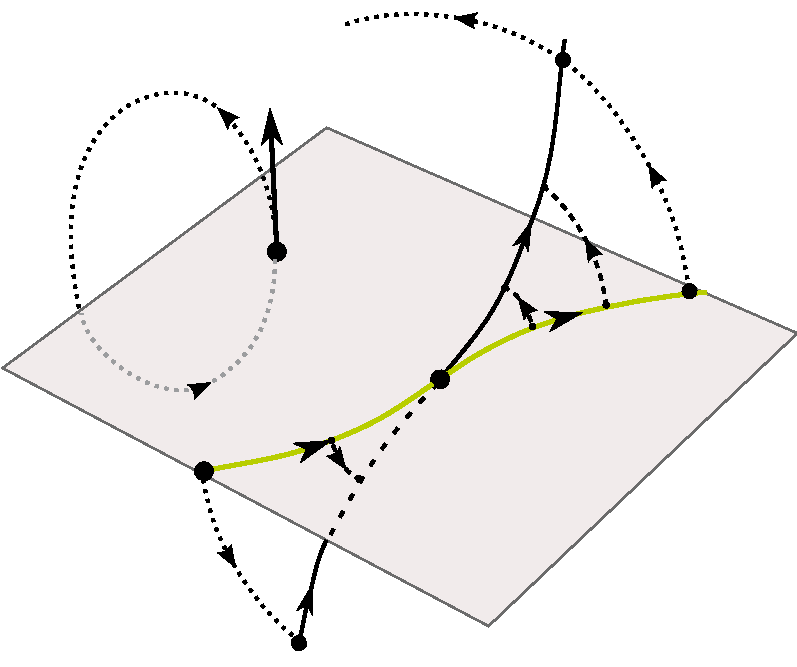
\includegraphics[width=\unitlength]{ReducTraj5.pdf}}%
    \put(0.09054399,0.38282057){\color[rgb]{0,0,0}\rotatebox{-30.34758661}{\makebox(0,0)[lb]{\smash{$\pSRed$}}}}%
    \put(0.57768586,0.29773425){\color[rgb]{0,0,0}\rotatebox{0.0313674}{\makebox(0,0)[lb]{\smash{$\sspRed(0)$}}}}%
    \put(0.59310014,0.69932675){\color[rgb]{0,0,0}\rotatebox{0.03136739}{\makebox(0,0)[lb]{\smash{$\ssp(\tau)$}}}}%
    \put(0.8268425,0.39772328){\color[rgb]{0,0,0}\rotatebox{0.03136739}{\makebox(0,0)[lb]{\smash{$\sspRed(\tau)$}}}}%
    \put(0.81220962,0.66529577){\color[rgb]{0,0,0}\rotatebox{0.03136739}{\makebox(0,0)[lb]{\smash{$\LieEl(\tau)$}}}}%
    \put(0.23150193,0.63610779){\color[rgb]{0,0,0}\rotatebox{0.0313674}{\makebox(0,0)[lb]{\smash{$\LieEl\,\slicep$}}}}%
    \put(0.37740434,0.49597258){\color[rgb]{0,0,0}\rotatebox{0.0313674}{\makebox(0,0)[lb]{\smash{$\slicep$}}}}%
    \put(0.3627714,0.69665188){\color[rgb]{0,0,0}\rotatebox{0.0313674}{\makebox(0,0)[lb]{\smash{$\sliceTan{}$}}}}%
  \end{picture}%
 \end{center}
 \caption{\label{fig:ReducTraj}
 % (b)
\Slice\ \pSRed\ is a hyperplane \refeq{PCsect0}
passing through the {\template} point $\slicep$,
and normal to the group tangent $\sliceTan{}$ at $\slicep$.
It intersects all
group orbits (indicated by dotted lines here) in an open
neighborhood of $\slicep$.  The full
\statesp\ trajectory $\ssp(\tau)$ and the \reducedsp\
trajectory $\sspRed(\tau)$ belong to the same group orbit
$\pS_{\ssp(\tau)}$ and are equivalent up to a group rotation
$\LieEl(\gSpace)$, defined in   refeq{sspOrbit}
(from \wwwcb{}).
 }%
 \end{figure}
      							\toCB
Ponder whether to use \reffig{fig:ReducTraj} (current, but not updated
yet), or Fig~{fig:slice} in ChaosBook.org
How it was drawn is described in
\\
dasbuch/book/FigSrc/inkscape/00ReadMe.txt

  \item[2010-12-06 PC]
% ES 2010-01-19  Rescued from FrCv11.tex flotsam:
{\bf Tessellation of the \reducedsp\ by two or many slices:
how to implement it?}
Our proposal is essentially to approximately
\HREF{http://en.wikipedia.org/wiki/Voronoi_tessellation} {Voronoi
tessellate} (see \HREF{http://en.wikipedia.org/wiki/Voronoi_diagram}
{wiki on Voronoi diagrams})
We have to study Roweis  and Saul\rf{RoSa00}
\emph{``Nonlinear dimensionality reduction by locally linear embedding.''}
A sobering fact: Roweis, assistant professor at N.Y.U., a young
star in the field and universally liked, jumped out of his Washington
Square apartment earlier this year.

 This tessellation is akin to the
%\HREF{http://en.wikipedia.org/wiki/Vector_quantization}
{`vector quantization,'} (`block quantization,'  `pattern matching quantization'),
a computer science data compression method where sets of points are
clustered by their distance to `prototype' or `reference' points.
In computer science and linear programming a related method
is called \HREF{http://en.wikipedia.org/wiki/Vector_quantization}{`vector
quantization,'}
    \PC{credit Sara A. Solla with this observation}
(`block quantization,' `pattern matching
quantization'), a lossy data compression method where sets of points are
clustered by their distance to `prototype' or `centroid' points.
The
method is `lossy,' as in the replacement of a point by its `prototype,'
one drops the residual, \ie, the Euclidean distance between the two. It
works by encoding values from a multidimensional vector space into a `a
codebook,' a finite set of values from a discrete subspace of lower
dimension; \ie, what in the theory of dynamical systems is called
`symbolic dynamics.' Only the index of the codeword in the codebook is sent, thus
conserving memory and increasing compression. Vector quantization
numerical algorithms are unlikely to be useful to us.

% in part clipped from
% www.cs.unm.edu/~terran/downloads/classes/cs529-s10/docs/pretest_soln.pdf
An (affine) hyperplane is the locus of points obeying the equation:
\[
\sliceTan{1}\sspRed_1 + \sliceTan{2}\sspRed_2 + \cdots + \sliceTan{d}\sspRed_d = c
\,.
\]
In vector notation $\braket{\sspRed}{\sliceTan{}{}^{(j)}}=0$. In the case
of a slice the extremal distance condition sets $c=0$, so all our slices
include the point at the origin, $\sspRed=0$, and are not affine. A
$(d\!-\!1)$-dimensional hyperplane embedded in a $d$-dimensional space
and passing through the origin is defined by a normal vector \sliceTan{},
a vector orthogonal to every vector in the hyperplane (\sliceTan{} is the
primary object, the {\template} \slicep\ secondary in this way of thinking).
The intersection of two hyperplanes is a $(d\!-\!2)$-dimensional
hyperplane - the `ridge, `boundary,' or `edge' where two hyperplanes
meet. The intersection is $(d\!-\!2)$-dimensional because every vector in
the intersection must be orthogonal to the normals of both hyperplanes.
It is a $(d\!-\!2)$-dimensional hyperplane which also goes through the
origin. If you are an ant crawling along the trajectory $\sspRed(\tau)$
symmetry-reduced with respect to the first slice, you do not need to
compute this hyperplane. Every so often you compute
$\braket{\sspRed(\tau)}{\sliceTan{}{}^{(2)}}$. As long as this number is
negative, you have not gone too far. The moment it changes sign, you the
ant have crossed ridge, we symmetry-reduce with respect to the second
slice, and the ant continues its merry stroll along the second slice. We
do not need to be very precise about the instant where we switch, as long
as we are far away form wither slice's singularity subspace, so the ridge
can be `fuzzy,' and the numerical check infrequent and cheap.

There is a rub, though - you have to figure out how to pick the phases of
different \template s $\sliceTan{}{}^{(j)}$ in such way that you somehow
minimize the distance from one to the next as you cross the ridge. We
proposed in \refref{SCD07} to use heteroclinic connections for that - they
fix the relative phases of different \eqva.


 \item[2010-01-19 ES: Roweis and Saul\rf{RoSa00}] is indeed a very interesting
  paper that got me thinking again -- so much that I took the day off to devote
  it to symmetry reduction.

  The main goal is to construct a global, low dimensional ``intrinsic''
  embedding of high-dimensional data based on locally linear transformations.
  I will mention the three steps involved very briefly (but they will only make
  sense once one reads \rf{RoSa00} or the more detailed \rf{SaRo02}):
  (1) compute for each state space point its
  closest neighbors (within the sampled data), (2) solve a costrained
  least squares minimization problem for the (local) linear transformation
  matrix $W_{ij}$ that most accurately reconstructs each data point
  from its neighbors. (3) Given $W_{ij}$ (only!) solve a second minimization
  problem for the coordinates of each data point in a new, lower-dimensional,
  global coordinate system. In practice this involves solving a sparse
  eigenproblem for the first $d$ eigenvectors, where $d$ the dimension of
  the embedding.

  Roweis and Saul argue that the transformations computed in step (2) are
  translation, rotation and scaling invariant by construction and certain
  constraints imposed. This would fit us very well, but do we really want
  to also compute a low dimensional embedding? In principle this is what we are
  after, but we also do not want to make any drastic approximation of the
  dynamics at this stage.

  One option might be to reduce only by the group dimension.
  However one has to consider at least as many closest neighbors
  in step (1) as the dimension of the embedding. Then I would think that
  the problem might be computationally very intensive.

  Another option would be to bypass step (2) altogether and use a local
  moving frame transformation to map the local neighborhood of (a few?)
  sample points to local slices, then use step (3) to construct a global
  coordinate frame.

  In any case we might need to work with a symmetry invariant norm for the
  minimization problems, rather than the Euclidean distance used in \rf{RoSa00}.

  I would be very interested to try something else in a system without symmetry
  (e.g. KSe in antisymmetric subspace). Take the sample points from a dense
  set of periodic orbits. Rather than computing the  local transformation
  $W_{ij}$ in step (2), use the Jacobian of the periodic orbits
  (or use something Lyapunov vector related, if we get into this).
  Compute the global embedding as in step (3). Does it faithfully reproduce
  the dynamics? Can we learn something about the dimensionality of
  the attractor (actually of the embedding manifold)?

  There are $\sim1500$ papers citing \rf{RoSa00} so it is impossible to track
  all of them down. The ones from physics and math are fewer and the only one
  directly relevant to us I could find is by Bollt\rf{bollt07}.
  It does however use a different pattern recognition method (called ISOMAP)
  to compute embeddings of various systems, including KSe in antisymmetric
  subspace (no continuous symmetry reduction there).

\item[2011-01-24 PC] I know about ISOMAP and have decided that for us
it is a bad idea. Will blog that some other time.

\item[2011-02-04 ES] But what do you think about this method of Roweis and
Saul? It seems to do much better than ISOMAP for pattern recognition.
The important point that distinguishes it from ISOMAP appears to be that
it respects spatial relationships between neighboring points and
also conserves lengths.

\item[2011-01-15 ES]
I cannot see how you go from \refeq{sliceSingl0} to  refeq{sliceSingl}.
Is $\sspSing$ still unreduced space point? How do you bring it to the
slice (if you do)?

\item[2011-01-15 PC] There is no group action involved. I wrote
``We shall refer to the $(d\!-\!2)$\dmn\ intersection of the two as the
{\em \sset} $S$.'' How can I write it more clearly?

\item[2011-01-15 ES] Sorry, I did not read it correctly. You might want to
add that this set was called singular set in
Siminos and Cvitanovi\'c\rf{SiCvi10} for that gem of a reader who would
read both papers. [PC: done]

\item[2011-01-24 PC] Made a claim in the slice \&\ dice article:
``
What about the fixed-point subspace $\pS_\Group$?
Because of it, the action of \Group\ is globally neither free nor proper,
\etc. All intersections of slices, ridges and {\chartBord s} contain the
fixed-point subspace $\pS_\Group$. Should we worry? Not really. The
objective of the \mslices\ is to freeze all equivariant coordinates; once
frozen, they together with the  $\pS_\Group$ coordinates span the
symmetry-\reducedsp.
''

Hope that is right. Have a further claim - it's easy to perturb away from
the fixed-point subspace $\pS_\Group$; in linear order the perturbations
commute, so equivariance implies the full reducibility of these
perturbations into block-diagonal components for each representations.
This is how it all started, with Ruelle\rf{ruell73}, but I think it is true
for \emph{all} perturbations from  $\pS_\Group$, not just the stability
of \eqva.

\item[2011-07-08 Predrag]
The $L^2$ norm of $\groupTan(u)$ is weighted by
the quadratic Casimir  refeq{QuadCasimir}. For \SOn{2} this is
$C_2^{(m)} = m^2$,
\beq
\oint \frac{d\gSpace}{2\pi}
     \, (\Lg u(\gSpace))^T \Lg u(2\pi-\gSpace)
= \sum_{m=1}^\infty m^2 \left(a_m^2 + b_m^2\right)
\,.
\ee{tangL2norm1}


\item[2011-07-08 Predrag]
Ridges are of Lebesgue measure zero, no way you would hit them.

We do not need to be very precise about the instant
where we switch, as long as we are away from either slice's singularity
subspace.


\item[2011-07-08 Predrag, from \refref{FrCv11}]                     \toCB
At this point it is worth noting that imposing the global and fixed slice
%\refeq{PCsectQ}
is not the only way to separate equivariant dynamics into `group
dynamics' and `shape' dynamics\rf{BeTh04}. In modern mechanics and even
field theory (where elimination of group-directions is called
`gauge-fixing') it is natural to separate the flow {\em locally} into
group dynamics and a transverse, `horizontal'
flow\rf{Smale70I,AbrMars78}, by the `method of
connections'\rf{rowley_reduction_2003}. From our point of view, such
approaches are not useful, as they do not reduce the dynamics to a
lower-dimensional \reducedsp\ $\pS/\Group$.

\item[2010-09-28 ES: Faddeev-Popov ghosts]                    \toCB
(moved to here from froehlich/blog)
\\
From my random readings, supposedly making up for my inability to attend
colloquia in French: Faddeev in a
\HREF{http://www.scholarpedia.org/article/Faddeev-Popov_ghosts}{scholarpedia
article} discusses the difficulties in Yang-Mills quantization that led
him and Popov to introduce fictitious fields, now known as
\emph{Faddeev-Popov ghosts}. The problem was that of gauge fixing,
essentially of working on a slice. Faddeev says:

\begin{ttfamily}
It was clear that the equivalence principle had to be taken into account.
In the functional integral framework, the equivalence principle implies
that one has to integrate over classes of gauge equivalent fields instead
of integrating over all fields $A_\mu^a$.

The choice of the representatives in the classes of equivalent fields is
realized by means of a gauge condition (gauge fixing), for instance,
\[
    \partial_{\mu} A_{\mu}^{a} = 0 .
\]
This condition defines a plane in the set of all fields, which is
intersected by the gauge orbits defined by
\[
    A_{\mu} = A_{\mu}^{a}t_{a} \to A_{\mu}^{\Omega}
            = \Omega A_{\mu} \Omega^{-1} + \partial_{\mu} \Omega \Omega^{-1} .
\]
In this context, the difference among abelian and non-abelian cases
becomes clear. In the abelian case, we take $\Omega(x) =
\exp{i\Lambda(x)}$ and a gauge orbit is defined by
\[
    A_{\mu} \to A_{\mu} + \partial_{\mu} \Lambda ,
\]
which is just a linear shift. Thus all the abelian orbits intersect the
gauge surface at the same angle.

In the non-abelian case, the gauge orbit equations are non-linear and the
intersection angle depends on the field parameterizing the orbit. It is
clear that this must be taken into account in the functional integral.
\end{ttfamily}

See the wikipedia link to put this in the proper context. As an abelian
case Faddeev lists quantum electrodynamics where the group is $U(1)$ (the
same as in \cLe\ if we think in terms of complex variables). As a
non-abelian example he lists the Standard Model: $U(1)\times SU(2) \times
SU(3)$.

Faddeev relies on the group being connected to write group action in
exponential form, as Stefan does. $\On{2}$ in Kuramoto-Sivashinsky is
non-abelian so I am worried that there might be more work required. Are
all non-connected compact Lie groups non-abelian and vice versa?

The weight factor Faddeev and Popov introduced might be helpful in
trace-formulas for non-abelian groups.

\item[2011-12-06 Roman] However,  ECS can be used to project
trajectories onto a low-dimensional visualization where coordinates $a^k_{i}(\zeit)$
are defined by the inner product
\beq
\label{coordinatesRG}
a^k_{i}(\zeit)= \frac{1}{V} \int_V {\bf e}^k_i(\zeit)^\dagger\cdot({\bf u}(\zeit)-{\bf u}^k(\zeit)) dV,
\eeq
%\pagebreak
where $V$ is the flow domain volume, ${\bf u}^k(\zeit)$ is the ECS closest to
the system state at time $t$, and ${\bf e}^k_i(\zeit)$ are basis functions
representing a set of unstable and weakly stable modes characterizing the
particular ECS.

\item[2011-12-06 Predrag]
Mhm - why are we introducing new notation for \statesp\
coordinates in \refeq{coordinatesRG}? I cannot imagine a situation in which one
would like to make the bases  ${\bf e}^k_i$ time dependent, ${\bf e}^k_i(\zeit)$,
and we mostly use ECS themselves to construct projections, as in
\reffig{f:ssptransient}, not their stability eigenvectors. If you are really
thinking of using ECS's ${\bf u}^k(\zeit)$ as \template s whose linearized local
charts compose a global atlas for the flow, they would not be time dependent,
but fixed by a set of Poincar\'e sections to \statesp\ points ${\bf u}^k$, and
the associated set of unstable and weakly stable eigenvectors (what are
"modes"?) ${\bf e}_i^k$ would also be confined to the Poincar\'e section, and
not time dependent. But I think this is way too sophisticated for referees to
wrap their heads around....

I propose you drop time dependence from ${\bf e}^k_i(\zeit)$ and ${\bf
u}^k(\zeit)$ and pass over all that in silence for now. Or perhaps keep the
formula as is, as neither the authors themselves have never sorted out
how the \po\ eigenvectors are to be used in practice.

\begin{figure}
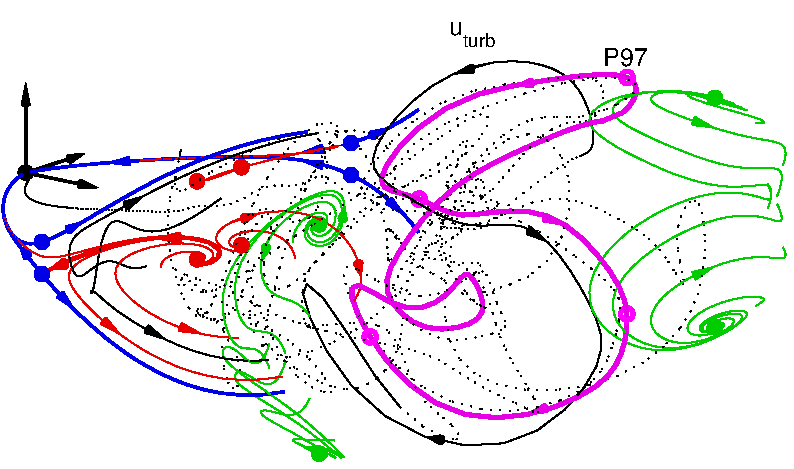
\includegraphics[width=0.4\textwidth]{P97portrait5}
\caption{
{\bf A state-space portrait of turbulent plane Couette flow.}
A turbulent trajectory ${\bf u}_{\text{turb}}$ (solid and dotted black
lines) shadowing the P97 periodic orbit (bold magenta line) and the
unstable manifolds (blue, red, and green lines) of symmetry-related
equilibria (solid blue, red, and green dots; the black dot at the origin
is the laminar flow state). Velocity fields corresponding to the open
magenta dots on P97 are shown in  reffig~{f:ssptransient2}. Dynamic
connections are shown as bold red and blue lines connecting different
equilibria (filled dots).
}
\label{f:ssptransient}
\end{figure}

\item[2011-12-06 John] Predrag's comment on \refeq{coordinatesRG} is on
target: it makes sense with the verbal description attached to it, but
the time-dependence of the basis set $e_i^k(\zeit)$ and the nearest ECS
$u^k(\zeit)$ is pretty confusing. The bigger problem is that the equation as
is reflects what we want to do, but doesn't the projection in
\reffig{f:ssptransient}, which uses a fixed basis based on four
symmetry-related ECS to produce a global portrait.


\medskip


\item[2011-10-28 PC~~] to Ashley: Once you have a \rpo\ reduced to a
slice, as in  reffig{f:MeanVelocityFrame} or  reffig{fig:M1OrbMarc}, you
simply take any point $\ssp \in \RPO{p}$, and trace its group orbit until
next time it crosses the slice; then you trace out the image of the
$\RPO{p}$ that you already have. That produces no less than the two slices of
the \rpo, as in your own \reffig{fig:sliceimage}, but in general more, as is
illustrated by the Siminos  reffig{ks22rpo16mf}.

In any case, keep going on the same group orbit of a point of the one and
only good \po\ and check whether there are further crossings of the
slice; each will correspond to yet another bad \po. Please check the sign
of the curvature for each traversal of the slice. If you
start from the good, nearest \po\ and track the curvature as you move on
the group orbit, you will go through zero curvature - such points mark
crossing the {\chartBord} $S$, \ie\ the border of the slice. It is verbotten
to cross on the other side - there you are outside our atlas of the
world.

\item[2011-10-28 PC~~] to Ashley:
    define the bulk velocity $U$ in the text, refer to it in
     reffig{f:MeanVelocityFrame}\,{(a)}. Isn't it sufficient to just plot
    $\vec{u}$, the deviation  refeq{NavStokesDev}? APW: It moves so
    rapidly that the plot would be an unfair comparison -- points
    sufficiently close to make smooth curves here plot as random points
    otherwise.  {\bf PC:}  I guess I do not understand. $\vec{u}(\zeit)$
    for $\RPO{36.92}$ traverses many $L$ streamwise lengths in period
    $\period{}=36.92$? Can you define $U$ in the text, refer to it by the
    equation number in the caption.
    {\bf APW} It traverses approx 8 times!  $U$ is the same $U$ used
    in the definition of the Reynolds number, hopefully clearer from
    slight rewording.

\item[2011-10-28 PC~~]: On using $\slicep$ as one of the coordinates: The
state vector $\ssp$ is not normal to \normVec(\ssp), as $\braket{\ssp
\Lg^2}{\ssp} = - \Norm{\groupTan(\ssp)}^2 \neq 0$, but can one use it to
produce from $\ssp$ the 3. local eigenbasis unit vector? Have not thought
that through. If we do that here, need to rewrite text leading to
\refeq{PCsectQ0}.

\item[11-11-04 APW~~] Why is curvature mentioned in the caption of
\reffig{fig:sliceimage}? {\bf PC:} As you look at the closest point on a
group orbit, distance increases in all moves away from it along the group
orbit, \ie, the matrix of 2nd derivatives of the distance function has
only positive eigenvalues. For any local extremum that is not a local
minimum, there are negative eigenvalues, \ie\ directions in which the
distance decreases.

\item[2011-10-20 APW~~]
 refFig{ks22rpo16mf} remains in the body tex,
which is what I was asking to be moved previously, and I'd prefer to omit
-- I think it'd be a real bugger to produce for the pipe orbits!
{\bf Predrag 111020} please give it a try for the $\RPO{36.92}$ - maybe
not so bad; hopefully not too many charts needed, especially if you use
as {\template} a point on $\RPO{36.92}$.
[see above: Ashley did replace it by \reffig{fig:sliceimage}]


\item[2011-10-28 PC~~] Marc, I've been pondering how to explain the
difference between using physical states to triangulate high-dimensional
\statesp s, and projections on a few primitive integration variables.
Maybe this helps (not suitable for this paper, but maybe you and Ashley
can see a way to communicate that fails me).

I will add this text to  refappe{appe:slice}, also including
    ``The problem we are facing is this: the inertial manifold
(or, more precisely for a dynamicist, the nonwandering set) is a
finite dimensional, presumably highly contorted nonlinear manifold
\citep{foias88}
embedded in our particular representation $\infty$\dmn\ vector \statesp.
Our strategy is: (1) shift the origin to a point embedded in the
inertial manifold. (2) construct an efficient atlas of the inertial manifold
by selecting a minimal set of \template s embedded in it, with associated
local hyperplanes that reduce the continuous symmetries (slices) and the
continuous time (Poincar\'e sections).
''

    ``More straightforward visualizations are based on choices of several Fourier
components  refeq{pipeDiscr} or other primitive basis elements as
coordinate axes for projections of the flow. They are appropriate for
small perturbations off laminar state, but such coordinate axes are (i)
arbitrary and discretization-method dependent, and (ii) point in
unphysical directions, far from turbulent states which in a highly
nonlinear flows are characterized by  many strongly coupled Fourier modes
of comparable magnitude.''

``The {\stateDsp} portraits are {dynamically intrinsic}, since the
projections are defined in terms of intrinsic solutions of the equations
of motion, and {representation independent}, as the inner product
\refeq{innerproduct} is independent of the numerical discretization.
''

\item[2011-10-25 John Gibson~~]  to Predrag: ``         \toCB
Chart or atlas is fine by me. We'll have some more 'splainin' to do for
the poor dumb plumbers. I think ``chart'' refers to be the set of
local maps from the manifold to a Euclidean space, and we will only ever
be dealing with maps between Euclidean spaces.
'' Here is what we wrote in a recent proposal: ``
{\em Patchwork dynamical models}. [...]
The long-terms goals of our research program are to develop this vision into
quantitative, predictive description of moderate-{\Reynolds} turbulence, and
to use this description to control flows and explain their statistics. The
first step, and the main subject of our theory proposal, is to build an explicit
instance of such a model for PCF in a minimal flow unit. A large set of
unstable periodic orbits for this flow have already been calculated\rf{CviGib10}.
We will compute the unstable eigenmodes of these orbits, continue their
unstable manifolds by time-integration of small perturbations, and thus map
out the conditions under which one unstable state transitions into another.
We will build a catalog of allowed transitions between ECS and calculate
the linearized dynamics in the low-dimensional unstable manifold about each
unstable periodic orbit. This will form a ``patchwork'' model of the turbulent
dynamics: an arbitrary fluid state will modeled by a low-dimensional
linearization in the unstable manifold of the nearest ECS, with the model
jumping from linearization about one ECS to another.
''


\item[2011-10-25 MA~~] back. Will work for food. I believe I understand
why Gibsonian coordinates are useful and accept their superiority; they
are well suited to look at phase space locally, while Fourier modes only
locally to the laminar state (i.e. useless in pipe flow). But many
people, including Mellibovsky \& Eckhardt (2011) and the sequel in the
arXiv do this. My suggestion was just to make a Fourier plot to compare
it to Gibsonian and be pedagogical...
\\
{\bf 2011-10-25 Predrag} Using Fourier modes is like standing in the
lower left corner of a soccer stadium, and trying to kick the ball which
is by the opposite goal. Best to try it yourself. You'll be enlightened
if you plot the $\RPO{36.92}$ as
$(\vec{u}_{327},\vec{u}_{253},\vec{u}_{199})$, compare with Ashley's
masterly physical projections. As to Eckhardt - I did the stupid thing
myself from 1996 to 2005 \refref{Christiansen97} until impossible, and we
realized that elementary ideas about vector spaces work better
\refref{GHCW07}.
\\
{\bf 2011-10-25 Predrag} the surprising thing about `physical' coordinates
(any better name to call them?)
is that they are so good \emph{globally}, that is what all plots in
\HREF{http://ChaosBook.org/tutorials}{ChaosBook.org/tutorials} are.


\item[2011-10-28 PC~~]
This has come to pass: China is getting modern at a frightening pace, I
have a \emph{lazy } Chinese student. He finally showed me on the screen
his undocumented Matlab plots of \KS\ \rpo s in co-moving frames. He does
not use any variant of my $\{\be_a, \be_s, \be_m\}$ orthonormal
`physical' basis  refeq{intrSspTraj} in spite of my many attempts to
explain it, and I suspects he does not understand what it is, until there
are plots that show the contrary.

\medskip

He plots \rpo s in `real space', meaning 3 components,
\[
\mbox{let's say } \{x_{47}, x_{48}, x_{49}\}
\,,
\]
of the 64-dimensional \KS\ discretization
vector that the integrator returns, with the mean {\phaseVel} per period
subtracted. \Rpo s do close into \po s. The shortest one looks like a
nice circle, longer ones are not a pretty sight. He has no clue that
there is FFT hidden in the integrator (or presumably what FFT is), so he
cannot plot your Fourier modes, but I think you see what the problem is
more clearly this way.

\medskip

It is as if Bjorn chose to look at 3 pixels of a
video image of one of his turbulent flows, and from that proceeded to
reconstruct the full turbulence. It cannot be done, even in principle;
it's like using a hot wire in a wind tunnel in 2011. What I offer to
Bjorn instead is a full resolution $3D$ snapshot of a turbulent state
(that is also a point in \statesp, but now the basis vector goes straight
through  it, and all pixels are retained), and ask him to compare his
measurement (a nearby point in \statesp) to my snapshot. That is a powerful
theory.

\medskip

Looking at a known \rpo\ is a bit misleading in this context. A circle
will close into a circle in any projection, as long the turbulent state
is global, as its \statesp\ trajectory generically has projection on all
of the $\infty$-many axes, but it is still a series of 3 pixels video.
You cannot work out the catalogue of turbulent states this way.

\medskip

Am I reaching you? If yes, can you put it in words that your colleagues
will understand? It is not about accepting superiority of Gibsonian
coordinates, it is about how to discuss this with fluid dynamicists. Even
Gibson does not understand this - since then he has fallen back to his
fluid-dynamicst's roots, it's all about bifurcations, snaking and plotting
things in the parameter-energy plane.


\medskip

The whole process of communal learning and myths fascinates me. Often one
encounters group mental states where all agree on something that is
patently a nonsense. Not just string `theory', or climate change deniers.
Plumbers' `energy' has no meaning other than that numerical people can
plot it because their codes happen to spew out Eulerian velocities. Ask
Bjorn to measure it... People click on a wiki, they exchange a nod of
agreement with a colleague and collectively psych themselves into
believing that they have understood. There are too many things, one
cannot learn them all, so groups work by consensus. It must have been
different 100 years ago when there were handful people interacting -
otherwise we still would not be using Cauchy's contour integrals and
quantum mechanics - those were inventions that really required exercising
neurons. Here we are picking axes in a linear vector space.

\medskip

But I digress...


\item[2012-02-21 PC]  I like the way this chaos class is working, and I
think we can put together some of the best class contributions into a
pedagogical article about sections and slices. And we have a chance to
publish this in a high quality issue of one of the better journals in the
field, Chaos:

\item[2012-02-21 Phil Holmes to PC]
We write in connection with the recent IUTAM Symposium on 50 Years of
Chaos: Applied and Theoretical, held in Kyoto, which you attended. In
addition to the Conference Proceedings to be published by Elsevier as
part of their regular IUTAM series, the American Institute of Physics
(AIP) has agreed to devote a special issue of the AIP Journal
\emph{Chaos} to papers representing a selection of the topics presented.
This is planned to appear as \emph{Vol 22 (4), December 2012}. So far 11
invitees have agreed to contribute papers; only one (David Ruelle) has
declined.


Based on your interesting presentation in Kyoto, we would like to invite
you to submit a paper for consideration for this special issue of Chaos.
Please let us know as soon as possible if you would like to do so, at the
latest, before Monday Jan 16th, 2012. Papers may either review a topic,
preferably including new results, or present entirely new, unpublished
results; papers should also reflect the topics and themes presented at
the symposium. All contributions will be refereed in the usual manner, as
for unsolicited submissions to AIP journals. At present we expect this to
require submission of the paper by \textbf{March 30th, 2012}, with
resubmission of revised papers during June 2012.


\textbf{[NOTE from Phil Holmes]}
Since some of the work you described has appeared in previous papers, in
particular that on channel flows with John Gibson, I would be especially
interested in the new results on symmetry groups hinted at in your
presentation.


\item[2012-02-21 PC to Phil Holmes]
Thank you for your kind invitation to contribute to the special issue of
the AIP Journal Chaos in connection with our "50 Years of Chaos". I am
sorry I am responding past your deadline, but I was not sure we would
have results interesting enough to report in this issue, results that
have not been written up for other publications. Now I am feeling more
confident that we can offer a novel pedagogical review of the symmetry
reduction by the method of slices (that I had described by its
application to one example, the pipe flows, in Kyoto), so I would like to
join this very fine group of contributors to the planned December 2012
Chaos.

\item[2012-02-23 PC] For instructions read
\texttt{siminos/atlas/Chaos-v1/00ReadMe.txt}. The deadline is

\textbf{April 16, 2012}

\item[2012-01-03  Predrag]
    experiment with \ensuremath{\hat{\ssp}}, \ensuremath{\bar{\ssp}} or
    \ensuremath{\tilde{\ssp}} as the \reducedsp\ coordinate.

\item[2012-01-27 Predrag]
    please, as few \template s as possible. And there should be no
    jumps in $\dot{\gSpace}(\sspRSing)$, none at all. We just need to
    make sure that the ridges between the \template s are sufficiently
    close to each the \template s, so that the {\chartBord s} are excluded. Once
    \template s are picked, the rest is geometry of hyperplanes (NOTHING to
    do with dynamics, only with the group theory) so checking whether the
    {\chartBord} is on the far side of the tile edge (ridge
    between two \slice s) is a linear computation, to be undertaken
    independently of dynamics.

    If the jumps are genuine and non-removable by refinements of slice
    charts, that's a big deal. It indicates that the generic turbulent
    orbit makes arbitrarily close passages to invariant subspace(s), and
    that is physical, not a chart artifact. Are there physical states
    that are like Hagen \eqv, but stream-wise deformed, \ie\ is there a
    nontrivial subspace invariant under the whole symmetry $\Group =
    \On{2}_\theta \times \SOn{2}_z$?

\item[2012-02-18 Predrag] clippings

This procedure has been devised by Poincar\'e in the context of celestial
mechanics, in the aim of reducing the analysis of long-term planetary
motion and its dynamic stability [Poincar\'e, Les m\'ethodes nouvelles de
la m\'ecanique c\'eleste 1892].

From \refref{AmLeAg06}:
``A linear system is $\dot{x} =Ax$ and an affine system is $\dot{x}
=Ax+b$, where $A$ is a constant matrix and $b$ is a constant vector.''
                                            \toCB

``
In the R\"ossler system, the switching is induced by the nonlinearity
which acts when the trajectory is sufficiently far from lower fixed
point, that is, beyond the threshold $x-c$ in the third equation. The
nonlinearity acts when the trajectory is sufficiently close to upper
fixed points where its converging spiral induces the folding by sending
the trajectory back to the neighborhood of lower fixed point along its
unstable manifold. Thus, the lower fixed point is mainly responsible for
the stretching and upper fixed point for the folding.
''

\item[2012-03-02 Predrag] Francesco likes my explanation why Euclidean
invariance leads to spirals. Imagine a thousands of marines parachuted
into Sahara desert an overcast night with no wind. Turn off their GPSes,
and order each one of them to march straight to Tripoli. The chance that
anyone will walk a straight line is zero - at best they will circle, or
spiral away from where they started. In presence of symmetry, and no cost
for moving along the group manifold, and no possibility to flip the
direction of motion, all motions will be drifting.

\item[2012-03-02 Predrag]
A Modest Proposal: create along with this article a Slice \& Dice
tutorial, like the \HREF{http://chaosbook.org/tutorials/index.html}{\pCf
one}. I believe Mathematica has ability to put user-orientable 3D
graphics into a browser, or HTML5 has that facility - that would make
slicing much easier to understand.

\item[2012-02-28 Predrag]
    The big problem with Ashley's %\reffig{fig:thetadot2}
    \template s
    is that they belong to the set of \reqva\ that has nothing to do with
    turbulence. It would be better to use points from $\RPO{36.72}$ and
    some \template s picked from most likely the turbulent trajectory
    states.

    The problem is that you never explain how you chose \emph{relative
    phases} between \template s. I think the way it should be done is
    that in the starting slice\ $\pS{}^{(1)}$, a local chart at
    $\slicep{}^{(1)}$, you plot both points corresponding to group orbits
    of other \template s, and keep checking the distance of
    $\sspRed(\zeit)$ to all $\slicep{}^{(j)}$. The moment one of them,
    let's say $\slicep{}^{(2)}$ is closer to $\sspRed(\zeit)$, you keep
    that $\slicep{}^{(2)}$ (that fixes the relative phase) switch to its
    slice\ $\pS{}^{(2)}$, and keep checking distances there. You cannot
    just pick a random set of points, one on group orbit of each
    {\template} - slices so constructed can sit anywhere in the full
    \statesp. It is not a technicality - it is the reason why the shift
    is still too kinky, and probably the reason why no good guesses for
    \rpo s embedded deeper in the turbulence have not emerged as yet.

\item[2012-03-09 Bryce Robbins]
After diligently working on properly charting the state space of the
complex Lorentz flow I have successfully produced an atlas whereby the
singularities have been removed from the reduced flow!

\item[2012-03-09 Bryce]
Now the only issue I am running into now is how to merge two successive
trajectories in a given chart. For example: I am currently using 2
charts, whenever the value of  $|\dot{\gSpace}|>1$.  I rotate the final
point in the iteration into the other chart and start integrating in that
respective chart.

\item[2012-03-09 Predrag]
Do you really mean  $|\dot{\gSpace}|>1$? That seems far from $|\dot{\gSpace}|
\to \infty$, and $|\dot{\gSpace}|=1$ could be perfectly physical, especially
in some other slicing problem. How about checking the sign of chart
border condition,
\(
\langle{t(\hat{\sspRed}(\zeit))}\vphantom{ }|\vphantom{}t'\rangle= 0
\,.
\)
When this expression has changed sign, you have gone too far - backtrack
and change the chart.

\item[2012-03-09 Bryce]
Every time the code breaks I append a large array of data for each chart
with the new trajectory data. After all is said and done I have two
arrays each containing a bunch of data that is disconnected in certain
areas (namely the points where the integration ended and started back up
again when a new starting point was rotated into the chart from the other
chart). If I just iterate once I can join each dot in a 3D list plot,
however, in the final data set the jumps prevent me from connecting these
lines. If I do draw in the lines connecting the points I end up with
lines streaking across the symmetry reduced trajectory which is of course
very undesirable.

Any ideas to mitigate this?

\item[2012-03-09 Predrag]
As how to connect the two charts - have to think. I thought they connect
continuously on the ridge (intersection of the two \slice\ hyperplanes).
They do not?

The main thing (without which there might be no paper) is showing that
two templates suffice to slice $\SOn{2}$ for complex Lorenz. Bryce has chosen
two points on the group orbit = time orbit of the {\reqv}. I
believe that is wrong, because in any slice all points on a
{\reqv} correspond to the unique {\eqv}.

My feeling is that the other template should be as far as possible but
within the non-wandering set: Something close to the {\eqv} at the
origin. Cannot be the {\eqv} itself, as it is in the fixed-point
subspace, and there are no group tangents there.

I am not sure one can find two charts that do the job - as I have not
done it myself. But if it is impossible, the explanation why not might be
very interesting....

\item[2012-03-12  Predrag]
a more winged title? Current one sounds like several previous ones...
``Revealing the geometry of chaotic flows by slicing'' (?)
A putative outline of the paper is in
\refsect{chap:outline}.

Goal: chart the \statesp\ explored by chaotic dynamics,
a curved manifold embedded in a high-dimensional \statesp.

Wandering around and about curved manifolds embedded in 61,506\dmn\ can
be a bit intimidating for the bravest of cartographers. We'll liberate
you from high-dimension phobia, teach how to chart these turbulent seas.

Cover the curved manifold by the shortest-distance sections (for time
recurrence) and \slice s (for continuous transformations). In the limit of longer
and longer cycles this leads to the usual curved manifold geometry,
measured locally by Euclidean distances.


\item[2012-03-16 Bryce]
I'm going to try to resolve this issue of choosing two sufficient charts
for the complex Lorentz flow over the course of the next couple of days.
Based on what I have computed, I have a feeling that it is possible and
if not we might simply need more than two charts as you've suggested. I'm
going to plot the \chartBord\ in both charts I choose to see
if they are even sensible before I go about computing the dynamics. When
I make some significant headway I'll inform you of my progress. If you
have any ideas that pop into to your mind in the meantime let me know and
I'll try to implement them.

\item[2012-03-16 Predrag]
slice is 4-dimensional, so the chart border is 3 dimensional - do not
know how to visualize that in any 2- or 3- dimensional visualizations.

Only thing I can think of is to track $\dot{\theta}$ for $\hat{x}(\zeit)$,
until it gets rather large, make sure it happened beyond the ridge to the
next chart.

\item[2012-03-09 Bryce]
As I am plotting the reduced state space trajectory in only three
dimensions (x1, x2, z) so I should be able to find the border on the
slice. I do not intend to visualize the four dimensional border in its
entirety but will project it onto 3 of the 5 dimensions. Will this be
sufficient enough to determine if the slice is a sensible slice?

%%%%%%%%%%%%%%%%%%%%%%%%%%%%%%%%%%%%%%%%%%%%%%%%%
% 2011-10-23 Predrag: ConicplaneSects.png
% from en.wikipedia.org/wiki/File:Conic_sections_with_plane.svg
% edited siminos/figSrc/inkscape/ConicplaneSects.svg
%
\begin{figure}\label{f:ConicplaneSects}
\centering
(a) %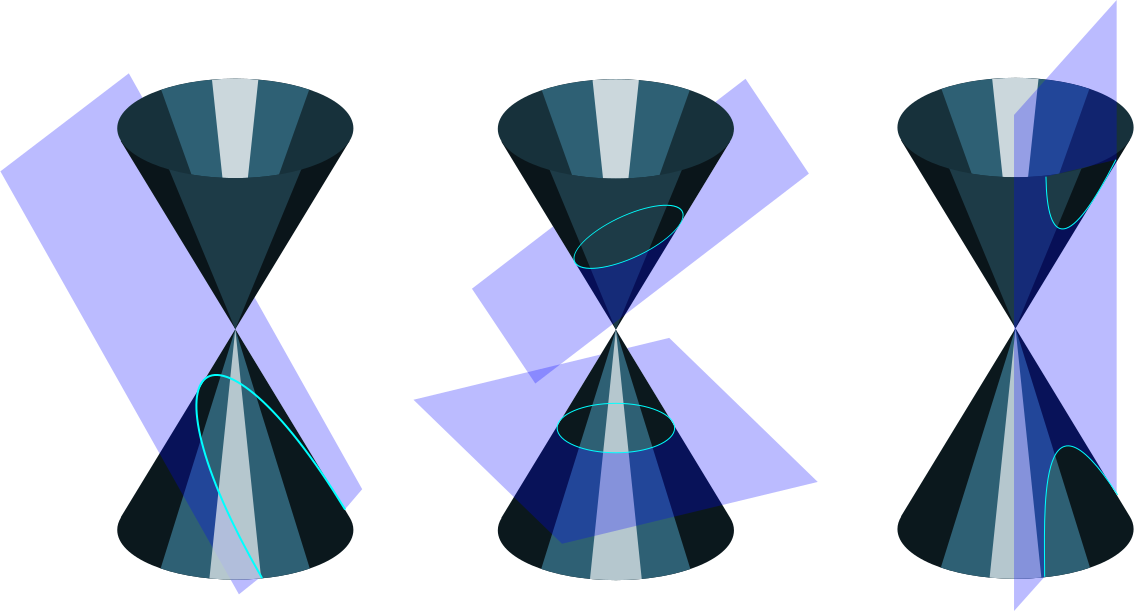
\includegraphics[width=0.45\textwidth,clip=true]{ConicplaneSects}
(b) %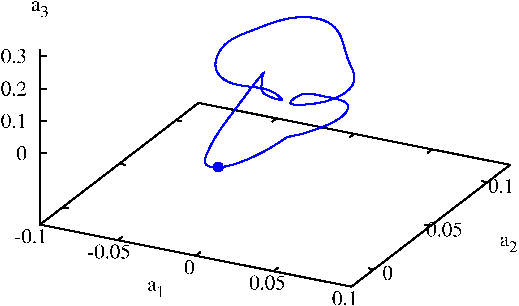
\includegraphics[width=0.45\textwidth,clip=true]{2841GO3b}
\caption{
(a) Conic sections (b)
}
\end{figure}
%%%%%%%%%%%%%%%%%%%%%%%%%%%%%%%%%%%%%%%%%%%%%%%%%%

\item[2012-03-11 Predrag]
Let's try to solve ChaosBook.org problem 3.2 (?) right, like any
high-school kid would do: look up
\HREF{http://en.wikipedia.org/wiki/Conic_sections}{Conic\_sections} in
Wikipedia, see \reffig{f:ConicplaneSects}.

\item[2012-03-10 Predrag to Daniel] I put soluChap10.pdf in Dropbox. In
the current edition the programs are renumbered. So far you have done:
\begin{itemize}
  \item[10.8]  An $\SOn{2}$-equivariant flow with two Fourier modes
  \item[10.10] $\SOn{2}$ equivariance of the 2-mode system
           for infinitesimal angles.
\end{itemize}
Next bunch of exercises to do:
\begin{itemize}
  \item[10.11] Visualizations of the 5-dimensional 2-mode system
  \item[10.22] 2-mode system in polar coordinates.
  \item[10.23] The relative equilibria of the 2-mode system
  \item[10.24] Plotting the relative equilibria of
           the 2-mode system in polar coordinates
  \item[10.25] Plotting the relative equilibria of
           the 2-mode system in Cartesian coordinates
\end{itemize}

Still have to make up exercises on group orbits, templates, slicing


\item[2012-03-18 Predrag]               \toCB
Use \reffig{fig:A27-pipeSymms} in ChaosBook.org. (to Predrag: remember to
copy them to dabook/book/Fig and FigSrc/). How it was drawn is described
in dasbuch/book/FigSrc/inkscape/00ReadMe.txt


% FIG. 11. A 2-chart atlas
\item[2012-02-25 Predrag to Chaos Gang]
It seems to take a workday to draw 3-4 figures, so the draft is still
problematic. But do please study \reffig{fig:A29-2slices}, it's a
concrete proposal how to slice the \cLf\ and the 2-mode model.

\item[2012-03-18 Predrag] I have added Siminos data (see {\bf [2010-07-12
ES]} above) to the Chaos Course Dropbox.com:
\\
          \texttt{SharedCode/CLErpos.dat}
            contains Evangelos Siminos data on four relative periodic
            orbits, symbolic codes 1, 01, 011, 001 you can use to test
            you code. The data is ordered as
            (T theta x1 x2 y1 y2 z Lambda1 ... Lambda4)
\\
          \texttt{SharedCode/CLEcycles4.dat}
            If you really want to go to town, a much larger set of
            relative periodic orbits, you can figure what is what by
            comparing with the 4-orbits data set above.

\item[2012-03-18 Predrag] My gut feeling is that a good 2. \template\ for
\cLf\ could be a point on the \cycle{01}-cycle; that is the short \rpo\
`furthest away' from the 1. \template\ \cycle{1}. \Eqv\ at the origin is
out, as it lies in the \Group-invariant subspace and has no non-zero
group tangents. \Template s should always be chosen fully equivariant,
otherwise they do not fix a slice.

\item[2012-03-20 Daniel]
Got the slices working for \cLf. Used the implementation from
ChaosBook.org ver. 13.7.3, sect. \emph{10.4.2 Dynamics within a slice},
rather than the post-processing method. Given a template my code can
slice away. I recreated figures 10.12 (attached) to check that it was
doing the right thing and they look pretty good.


\item[2012-03-20 Predrag  to Daniel]
You are still in the larval, single slice stage - if you look at your 2.
plot, (track magnitude of $\dot{\theta}$, \etc) you will find out that
you are going through singularity and jumping by $\Delta \theta = \pi$
every time you do it. All mindless integrators cheat their way through
this singularity, but if you want to see it in detail, have a look at
Figs. 3 and 4(a) in
\HREF{http://www.cns.gatech.edu/~predrag/papers/preprints.html\#FrCv11}
{www.cns.gatech.edu/$\sim$predrag/papers/preprints.html\#FrCv11} (and do
not ever publish figures so ugly - Stefan\rf{FrCv11} got waiver as an
undergrad and a mathematician).

\item[2012-03-20 Daniel]
What do you think would be the most productive next step? Modify the code
to slice the 2-mode system? Take slices of the complex Lorenz system with
templates that are not the {\eqv} solution? Try to Poincar\'e
section the slices? Please advise. In the meantime, I'll clean up my code
so it makes sense to people when I post it.

\item[2012-03-20 Predrag  to Daniel] Let's get a 2-chart atlas working, then
we move to the next thing...

\item[2012-03-21 Daniel  to Predrag] Ok. Got the tunnel working so I can
read this stuff at home and actually take the time to blog. Couple of
comments:

Who is doing what? It seems like there is some duplication of effort in
this endeavor. One can sort of dig around the various blogs and such and
infer what people are working on, but it's kind of hard to tell. It seems
like at least Bryce and I are chasing the same result.

\item[2012-03-21 Predrag]
It's not duplication, for the students it's education. Ideally, everyone
in the calls should be able to do this (there are only two students who
are not seriously working), and anybody who contributes significantly to
the paper can be a co-author. The goals are very modest: explain
pedagogically the course lectures on symmetry reduction, in two steps:
(a) Carefully re-examine and illustrate on R\"ossler flow what is one
really does when one sections time trajectories: (b) Repeat the same on
slicing the the group orbits, illustrate by \cLf, both models with high
quality figures. I hope that by the students making sure the exposition
is pedagogical it will much more so than my papers have been.

In your case (and equally so for Radford and Chris, but they seem not to
have gotten the memo) I hope you will find this very helpful in your
research, so understanding is much more pressing than for the Chaos
Course.

I do not understand why it has been so difficult - I think that the
problem is that the senior people assume they have been knowing this, and
none of them do. I speak with some authority, as I know much more group
theory then 99\% of physicists, and I had not known these methods. Turns out
that nonlinear group theory is to linear, quantum mechanical methods what
linear ODEs are to nonlinear ones.

Spent two hours with Roman and Mike (sorry, should have thought of
calling you in to Roman's office, but I had assumed it would take only 15
minutes), and my chaos class understands this better than the pros. Maybe
it does.

\item[2012-03-21 Daniel]
It is also not totally clear to me where I should be saving code,
figures, blogging, etc., so that it is most useful to the group effort.
Predrag, please advise.

\item[2012-03-21 Predrag]
An attempt in \refsect{chap:outline}, edit as you see fit.

\item[2012-03-21 Daniel]
I had read the stuff in DasBuch about the singularities. I just wanted to
make sure that I was on the right track. Anyway, I guess the idea is to
jump to a different chart (hyperplane associated with a single template)
whenever you get close to the singularity (probably way before then, and
more like when you are closer to another template on another chart,
right?)

\item[2012-03-21 Predrag]
ChaosBook chapter is two years out of date - the current wisdom was only
given in my lectures and shuld be written up in the
siminos/atlas/atlas.tex paper. I will rewrite ChaosBook chapter after we
finish this paper and clock up a few more cutting edges research
breakthroughs. Please try to implement atlas construction as outlined in
\reffig{fig:A29-2slices}.

\item[2012-03-21 Daniel]
Is the 2-mode system still of interest or should we put that on the
back-burner and focus on the \cLe, even if the relative equilibria are
all circles? I've been writing two versions of every piece of code, one
for the complex Lorenz system and one for the 2-mode system (which is
still lacking a ``good'' set of parameters that make it nice and
chaotic). It's not too much work to make one once you have the other, but
there are details to be addressed, so work would go faster working on a
single problem.

\item[2012-03-21 Predrag]
Atlas for \cLe\ is the top priority. The 2-mode system is experimental,
maybe you can get a more interesting system from some truncation of the
2D Kolmogorov flow. That is totally open.

\item[2012-03-21 Daniel]
From some of the most recent comments copied from pipes/blog suggest that
Rich (I'm assuming Kerswell?) has been looking at periodic orbits in 2D
Kolmogorov flow. Perhaps, the third floor 2D crowd should be in touch
with these guys. Do Mike and Roman know about this?

\item[2012-03-21 Predrag]
Sorry, maybe it is my fault - I just assume everybody tracks the current
literature, I should have told them in person. Here is another relevant
blog entry:

{\bf 2011-05-18  Rich Kerswell} Read Irene Moroz, Geophys. Astrophy Fluid
Dynamics vol 105, 273-286, 2011, \emph{Unstable periodic orbits in 4D
Faraday disk dynamo}. Might give you a 4-dimensional dynamical system
which is chaotic and can be reduced to a 3\dmn\ \statesp; easier to
visualize than {\cLf}.

Kerswell papers are published and easy to find; if you learn something,
please summarize it here for the rest of us.

\item[2012-03-26 Daniel] Looked through various publications by I. Moroz
et al. about a 4D model for a dynamo model that Rich Kerswell had
mentioned as a possible candidate to replace complex Lorenz. This model
has chaotic regimes and some terms that break its discrete symmetries.
There are no continuous symmetries (although don't explicitly say that
they aren't there either), so this might not be a good candidate to
replace complex Lorenz as a toy model for slicing and dicing. However,
the fact that they can find (exact, rather than relative) periodic orbits
probably means that the system does not have continuous symmetries. If it
did it'd be very hard to find exact periodic orbits.
{\bf 2012-03-27 Predrag} I agree, this baby is DOA. Scratch that.


\item[2012-03-19 Predrag~~] Please study \reffig{fig:A29-2slices}, it's a
concrete proposal how to slice with several templates. Their relative
phases matter.

\item[2012-03-21 Marc~~] \refFig{fig:A29-2slices} is a very neat solution
to the problem of how to decide when to switch templates. Still, the
main problem I see is that currently the only useful templates that we
have are S2U and perhaps LB, but we have no good template
representative of the upper turbulent region. So even if we can switch
templates in a clever way I don't see how we can improve our chart without
adding new templates. Predrag if you make it a webinar I'll join.

\item[2012-03-21 Predrag~~]
The brilliant thing is that now everything is rigid - once you have
chosen templates, the ridge between them is unique and fixed, and all is
based on the same principle of choosing the minimal distance solutions. I
have illustrated this only for a pair of templates in
\reffig{fig:A29-2slices}, because the trajectory always switches slices
pairwise - it does not matter how many templates there are, you keep
testing. Checking whether the {\chartBord} is on the far side of
the ridge between two \slice s is a linear computation, to be undertaken
independently of dynamics. For a reduced trajectory moving in
$\pSRed{}^{(1)}$ slice one only has to keep checking the sign of
\[
\braket{(\sspRed(\zeit)- \slicep{}^{(2)})}{\sliceTan{}{}^{(2)}}
\,.
\]
Once this changes the sign, the ridge has been crossed, and from then on
the trajectory should be reduced to the $\pSRed{}^{(2)}$ slice. Test
every so often,you just have to switch before you hit the current
\template's {\chartBord}). There is no need to pinpoint this crossing
accurately, as long $\sspRed(\zeit)$ stays well clear of all \chartBord
s.

If your chart fails before, you insert another local chart between the
two \template s. The way you do this is by finding a longer cycle that
winds around the two templates. That you do in the two local Poincar\'e
sections, one centered on each \template. In sections, these are fix
points (let's say \cycle{0} and \cycle{1}). Then the cycle points
\cycle{01} and  \cycle{10} serve as interpolating \template s.

Under {\color{red} NO circumstances} use
\HREF{http://samuel-beckett.net/Waiting_for_Godot_Part1.html} {Waiting
for Godot} as an excuse to postpone writing up the paper. We have plenty
completed work to write about, and at such time that we make further
significant progress, we will have more to write about.

What we are doing is charting a curve manifold the way non-Euclidean
geometries work; the Euclidean metric becomes infinitesimal notion, we
are approaching this by successive refinements - addition of every \po\
embedded in the ergodic sea is a successive refinement. It nicely blends
into Chat\'e-Gineli-Siminos-\etal\ approach, and it really feels like the
right thing.

\item[2012-03-22 Bryce]
After trudging in excess of 4 hours through my most recent attempt to
slice and dice I'm laying it to rest... The cycle points seem to suffer
the same discontinuity in $\dot{\phi}$ and switching between the
{\reqv} point $\REQV{}{1}$ and any of the four cycle points is not
producing desired results. In general, the sign of
$\langle(\sspRed(\zeit)- \slicep{}^{(2)})|\sliceTan{}{}^{(2)}\rangle$
either occurs too soon (on the order of $<.1$ units of time)  or too late
(we've hit the chart border!). I'll continue to probe this issue at later
time.

\begin{figure}
\begin{center}
  \includegraphics[width=0.35\textwidth,clip=true] %,height=0.5\textheight
  {CLEchaotic}
  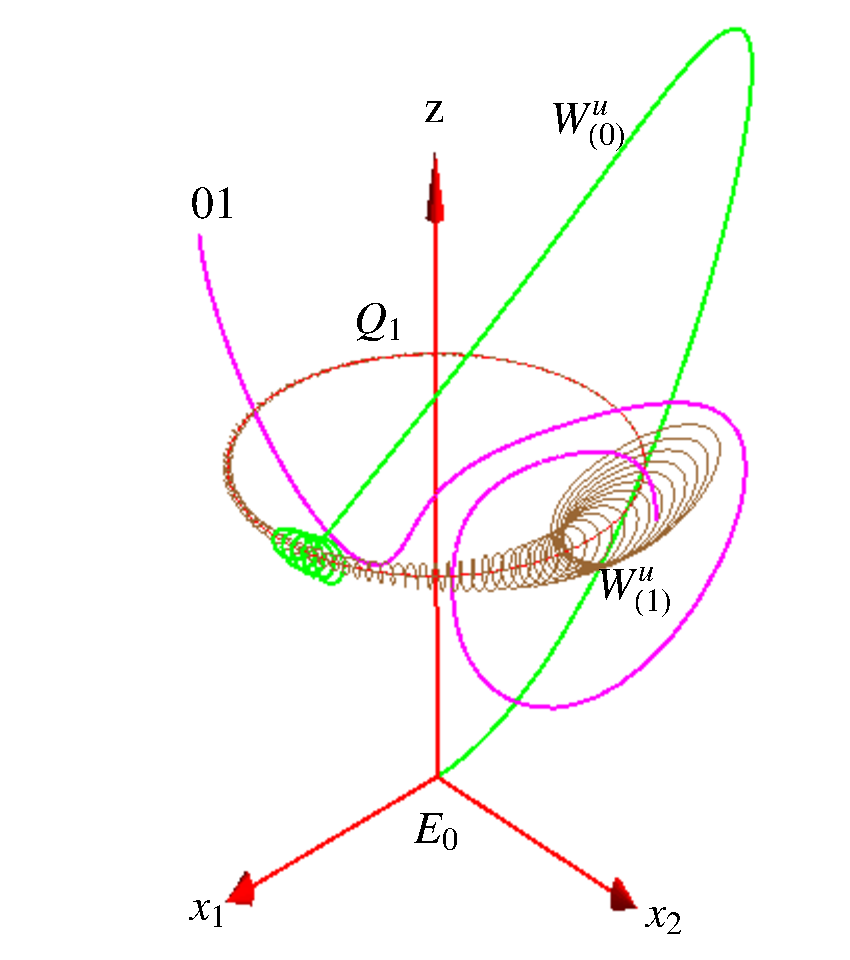
\includegraphics[width=0.35\textwidth,clip=true]
  {CLEcompact}
  \\
  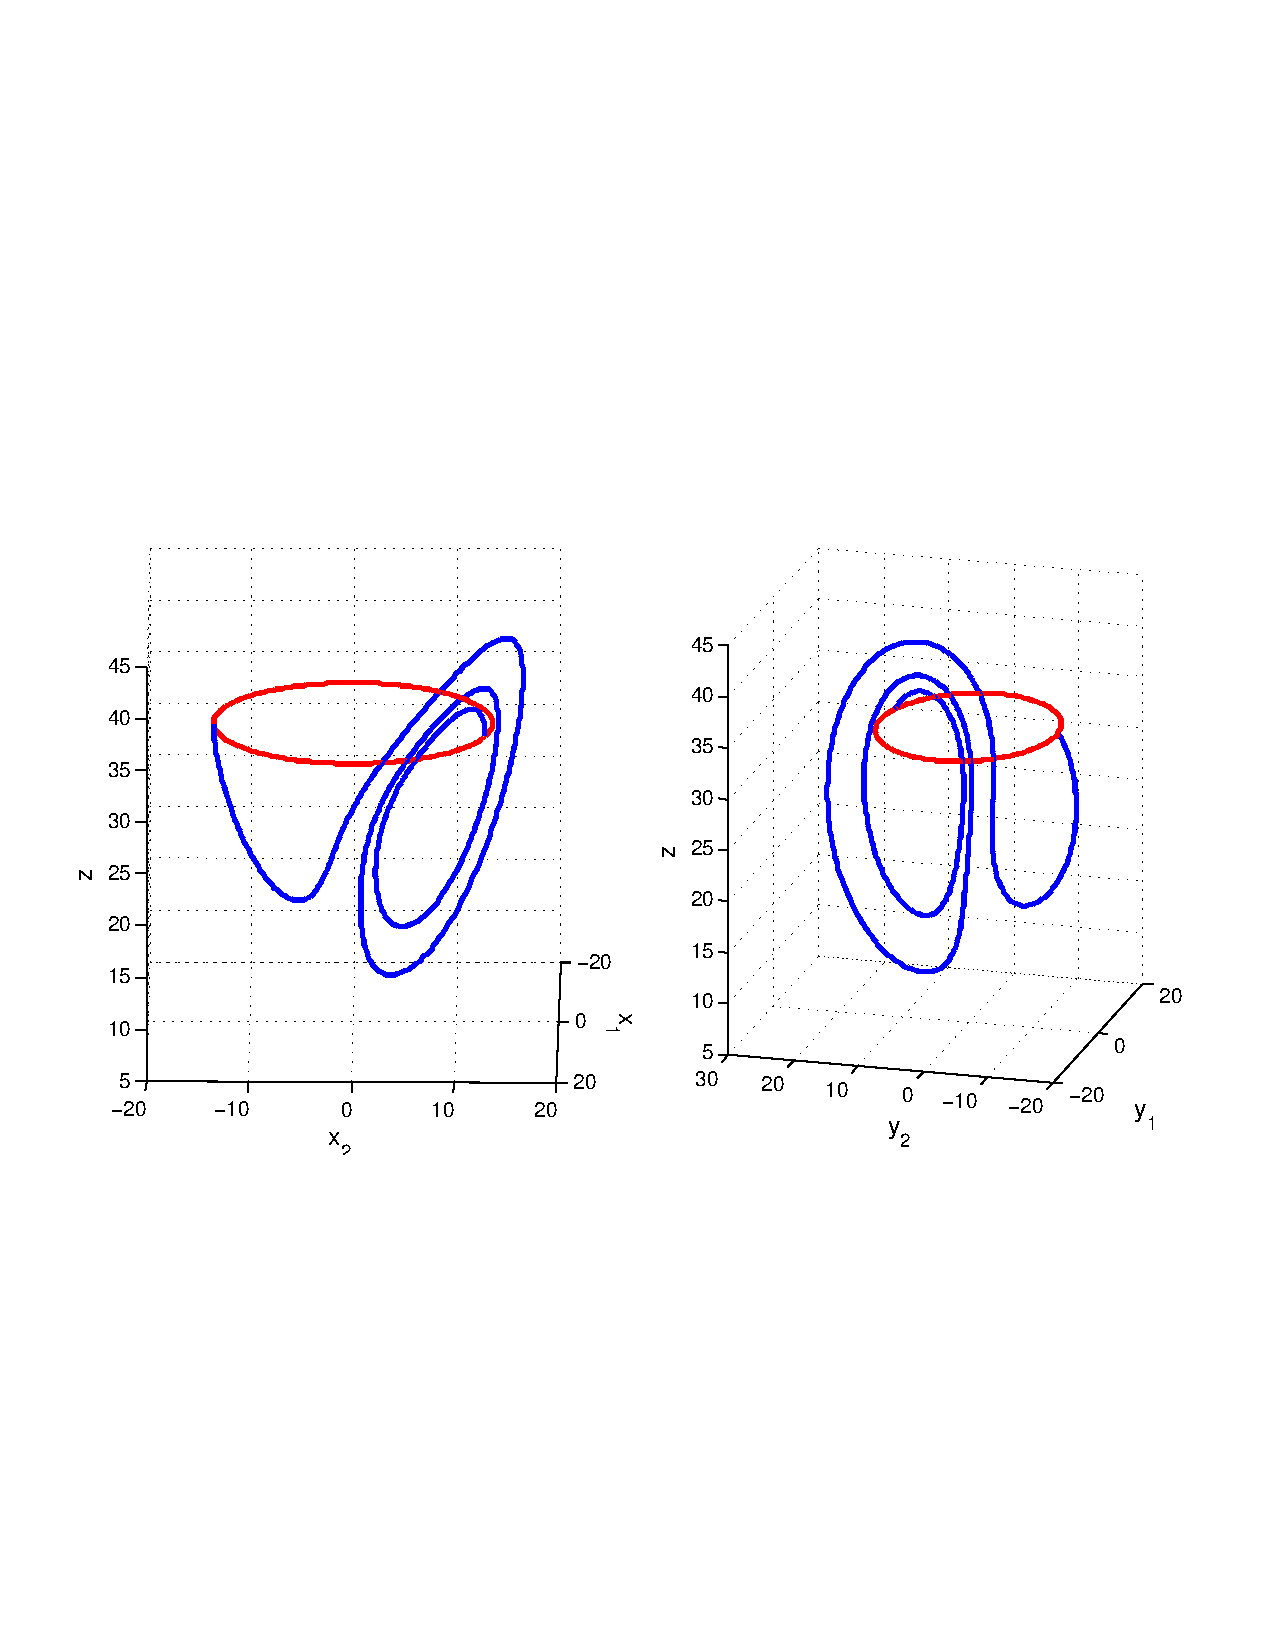
\includegraphics[width=0.7\textwidth]{CLERPO001}
\end{center}
  \caption{
\CLf:
(a) (b)
Continuous symmetry induces drifts: generic chaotic trajectory (blue);
$E_0$ \eqv;
$E_0$ unstable manifold - a cone of such (green);
$\REQV{}{1}$ \reqv\ (red);
$\REQV{}{1}$ unstable manifold, one for each point on $Q_1$ (brown);
\rpo\ \cycle{01} (purple)
(c)
    The \rpo\ \cycle{001} is shown in blue.
    The group orbit of the initial condition is shown in red.
}
\label{fig:CLERPO001}
\end{figure}

\item[2012-03-22 Daniel~~]
Citing Bryce's email: ``Have you worked with the cycle data Predrag
dropped into the box? I've plotted the trajectories without symmetry
reduction and they seem ok (for some reason they aren't closing
completely and I have to plot them for twice the period).''

Answer: I'm pretty sure that the Simino's data as posted by Predrag in
the DropBox is fine. It is important to remember that these are
\emph{relative} periodic orbits and return to the group orbit of the
initial condition, not to the initial condition itself. See
\reffig{fig:CLERPO001}, for example. Some of the orbits given
\emph{almost} close but actually don't (in which case they would be
periodic orbit, rather than relative periodic orbits). For example
$\theta$ for $\cycle{011}$ is $-0.0296\, \sim \,0$, so the orbit looks
like it almost closes. For $\cycle{1}$ is $\theta = 3.1669\, \sim
\,\pi$ so when you integrate it for twice the period it looks like it
closes (but doesn't if you look carefully).

Citing Bryce's email: ``However, when I symmetry reduce them using the
non-post processing method the integrator jumps shortly into the
integration and the point falls back onto the strange attractor rather
than following it's periodic orbit.''

Answer: I'm assuming you mean calculating the dynamics  on a slice using
$\REQV{}{1}$ as your template. What is happening is that at some point the
template becomes a bad template and the denominator for the {\phaseVel}
$\dot{\gSpace}$ equation blows up. Your integrator will just integrate
across this since it never quite hit the singularity on the nose. You
need to stop your integration before this happens, switch templates, and
continue calculating in the new slice. Ideally, you want to try and stop
way before this happens as we discussed with Predrag yesterday.

If you read the caption for the symmetry reduced orbits you'll notice
that it says that there are some nasty singularities that need to be
addressed.

\item[2012-03-22 Predrag~~] Thanks Daniel, that clears it up - Evangelos
is vindicated. For Chaos Gang article we will need a figure like
\reffig{fig:CLERPO001}\,{(c)}, but for the purple cycle \cycle{01} in
\reffig{fig:CLERPO001}\,{(b)}, together with the (red) \reqv\
$\REQV{}{1}$. Make it pretty, at least as pretty as
\reffig{fig:CLERPO001}\,{(b)}, and \emph{small} *.pdf. Save the
program in siminos/figSrc, document it (what it is, how it works) in
siminos/figSrc/00ReadMe.txt.

Next, plot \cycle{01}  in your single slice program - I sure hope it
jumps at the far end of the slice hyperplane, and that you verify it
reaches beyond it \chartBord. Take the furthest point beyond the jump,
use it as template, do as \reffig{fig:A29-2slices} says. Either you
triumph, or you explain what is wrong with my line of thought.

Keith stopped by - is thinking, but will be out of action for next few
dates.

\item[2012-03-22 Predrag~~] To Bryce and Daniel: I think yesterday's
argument about fixing the Poincar\'e section by  minimizing the distance
\beq
\Norm{\ssp(\zeit) - \slicep)}^2
\ee{minDistPinc}
under time variation is wrong.  Try it out yourself.

\item[2012-03-23 Keith~~] Fixed my code for slicing, and am working on
checking 2 slices; need to think about nature of edge.  Bryce, I think
you and I are on the same page about running into the troublesome areas
before being able to transfer from 1 slice to the other.  Have you
troubleshot this and I missed it?  I will think about this and will check
this while away; perhaps I am misunderstanding these discontinuities.

\item[2012-03-23 Predrag~~] I hear you, hope that the pain is soon replaced by
enlightenment.


\item[2012-03-23 Daniel~~]
Generated figure (+code) for figure described by Predrag on 03/22.

\item[2012-03-23 Predrag~~]
(a) Draw also the group orbit of the two ends of \rpo\ \cycle{01}.
(b) Get rid of the funky matlabian grids, color label up right.
(c) $z$ axis must start in (0,0,0,0,0), otherwise figure makes no sense.
(d) Try drawing something like 5 to 20 periods \period{}; It should trace
out a torus, I'm curious what it looks like. Do not run it for time
$20\,\period{}$; restart at multiples of the \rpo\ shift $\gSpace$, so
the exponential instability cannot build up.
(c) Draw the \po\ \cycle{01} in the slice of the \eqv\ $\REQV{}{1}$.
Hopefully it will jump.

\item[2012-03-23 Daniel~~]
Not sure how to make the axes look like arrows as in
\reffig{fig:CLERPO001}\,{(b)}. If anybody knows how to do this, let me
know... I tried looking into drawing arrows in Matlab, but the
documentation does not say anything about drawing them in 3D plots.
Basically, it just draws 2D arrows in the plane of the figure (rather
than the 3D space).

\item[2012-03-23 Your Personal Googler] click on this link:
\HREF{http://stackoverflow.com/questions/1962332/how-to-draw-vectors-physical-2d-3d-vectors-in-matlab}
{how-to-draw-vectors-physical-2d-3d-vectors-in-matlab}

Also, try this answer to this question
``I'm trying to plot 4 curves in a 3D plot with Matlab (I used
plot3d(xmatrix,ymatrix,zmatrix)), and I would like to have the 3 axes
meet at point (0,0,0)?''
\begin{verbatim}
First get the axis limits with
>> lims = axis;
Then plot them
>> hold on
>> plot3(lims(1:2),[0 0],[0 0]) % for x-axis
\end{verbatim}


\item[2012-03-23 Daniel~~]
Not 100\,\% sure how to make it look good and have a small file size.
Anyway, put the code in siminos/figSrc if anybody wants to play with it. It is
called TWand01.m.

Going back to what Keith just said, if you look at this figure
\ref{fig:TWand01}, you can see that \cycle{01} starts kind of far
from the group orbit of $\REQV{}{1}$. Maybe it would be smart to
integrate until you are closer, pick this as your initial conditions, and
then try to slice away. Just a thought...

By the way, if you think the previous idea makes sense, you should use
\\
$\REQV{}{1} = [1.096726099509717   8.414075687850639   1.173217076809554   8.404104297941718  26.998899999999999]$
\\
(Siminos \cycle{01} data set point rotated by $\theta =
4.851093070122474$) ({\bf Predrag to Daniel}: you really mean
$\REQV{}{1}$? Or you mean the second template $\slicep{}^{(2)}$, rotated
into the slice of the first template, \reffig{fig:A29-2slices}? Why
should I be rotating the first \template? I should rotate the starting
\rpo\ point into the $\REQV{}{1}$ slice instead?) and use
$\sspRed_{01}(0) = $
\\
$[0.811309512488248, 5.424865982998012, -0.120847013076036, -0.118120467113914, 30.380669763749523]$
\\
I got these by integrating Siminos's solution and finding the closest
pass between the group orbit and the time trajectory of \cycle{01}.

\begin{figure}
\begin{center}
  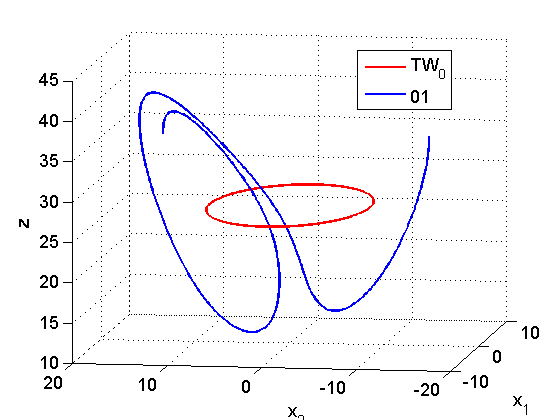
\includegraphics[width=0.35\textwidth,clip=true]{TWand01}
\end{center}
  \caption{
  One period of the relative periodic orbit \cycle{01} in the full
  space and the group orbit of the \reqv\ $\REQV{}{1}$ (red).}
\label{fig:TWand01}
\end{figure}

\item[2012-03-23 Predrag to Daniel]  Not the closest, use as the 2nd
\template\ the cycle-point on the \cycle{01} \po\ (in the slice of
$\REQV{}{1}$) which is the furthest away from $\REQV{}{1}$. Then the
two charts together will give the optimal cover over the whole \cycle{01}
trajectory.

\item[2012-03-23 Mike~~] Slicing 2d turbulence....recent result: it turns
out that the three known equilibria for the problem \emph{do} live near
the turbulence in state space----one realizes this only after accounting
for all discrete and continuous symmetries....for each {\eqv}, there
are 8 different copies (due to the discrete symmetries), but only two
distinct group orbits (4 copies lie on one and 4 lie on the
other)..... one of the group orbits is far away in \statesp\ from
turbulent trajectories that we've computed so far (only a short time
sequence), but the other group orbit intersects the same region of state
space as the turbulence.  This story is true for all 3 equilibria, but
the intersections occur at different regions for each {\eqv}. Next
step... check to see if the corresponding elements of the group orbit
`near' the intersections work as good templates for slicing.....stay
tuned.

\item[2012-03-23 Predrag~~] (Daniel, I fear you are carrier pigeon until
we get the fessor weaned off shooting random emails - he knows how to
subvert, he has done it on our grants: schatz   afosr07, and he gets
svn update messages)
\\
Please, you have to write down explicitly what the symmetry group of your
2D flow is. Use the wisdom of
\HREF{http://www.cns.gatech.edu/~predrag/papers/preprints.html\#n00bs}
{Halcrow}\rf{HGC08} (Sect. \emph{3. Symmetries and isotropy subgroups})
as the template. We put some thought into it, so lets not invent more
random notation. Discrete cyclic subgroups such as \Zn{2} are not the
symmetries of your flow, they are only symmetries of sets of solutions,
as \SOn{2} contains an infinity of discrete cyclic subgroups \Zn{m}, and
\On{2} contains an infinity of discrete dihedral subgroups \Dn{m}; for a
small cell, dissipative flow only a finite number of small $m$ \eqva\ can
be realized. If in the symmetry reduced \statesp\ $\pS/\SOn{2}$ all these
map to the same \eqv, you do not count them as discrete symmetries. My
intuition is that these are not physical, the important solutions are
\reqva\ which have no such discrete symmetry.

I suspect you have one or two parity operations (in the notation of
\refref{HGC08}), or one reflection and one $\pi$-rotation. All this
'shift-and-reflect' nonsense comes from guys like Waleffe who get a
migraine if you say words `Group Theory'; they only looked at few special
solutions, the general theory is much prettier and more systematic than
that.

\item[2012-03-24 Predrag to Daniel]
I have split \reffig{fig:A29-2slices} into
\reffig{fig:A29-2tmplts} and \reffig{fig:A29-2slices}, added a panel to
aid visualization. Now I think you were right in the above proposal to
Bryce:
use as the 2nd
\template\ the cycle-point on the \cycle{01} \po\ (in the slice of
$\REQV{}{1}$) which is \emph{the closest} to $\REQV{}{1}$. Otherwise
the ridge between to charts includes the $\pSRed{}^{(1)}$ {\chartBord}
and one cannot get from one \template\ chart to the next \template\ chart.
Hopefully the 2. chart reaches far enough that the whole \cycle{01}
trajectory is covered. If we are lucky, the whole strange attractor is
covered by this 2-chart atlas.

 \begin{figure}
 \begin{center}
(a)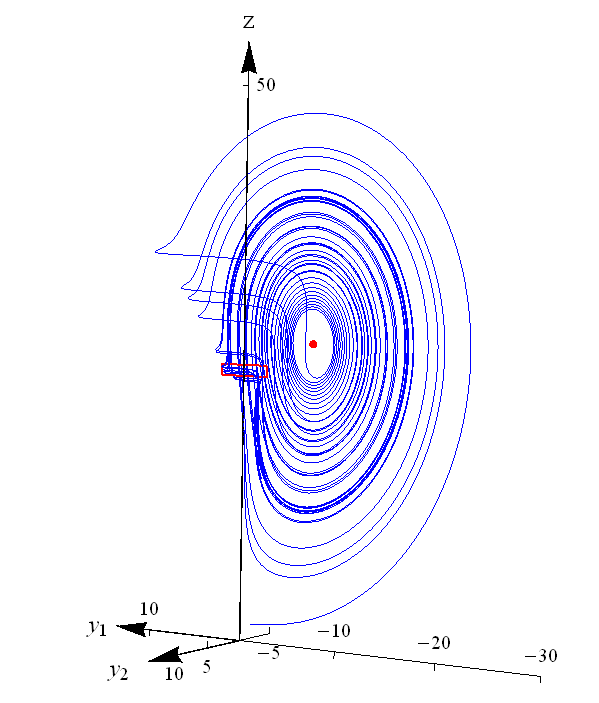
\includegraphics[width=0.32\textwidth]{RedTrajNoPlane1}%
~~~~~~~~
(b)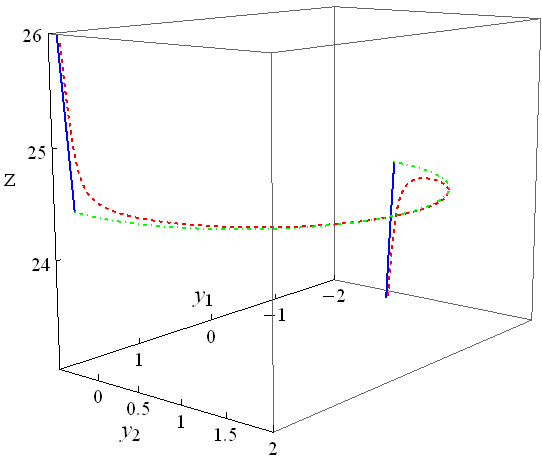
\includegraphics[width=0.42\textwidth]{singpass1}%
 \end{center}
 \caption{\label{fig:Fullspace} % first frame  in FrCv11.tex
    % Former {CLEreduced} \label{fig:RedTrajNoPlane1}
(a) The \cLe\ strange attractor plotted in the \slice\ hyperplane
\refeq{PCsectQ0}, defined by the group tangent $\sliceTan{}$ given in
\refeq{exmplTempl}. In the \reducedsp\ \reqv\ $\REQV{}{1}$ is reduced to
\eqv\ $\EQV{1}$. Both Matlab and Mathematica interpolate by straight lines
through the {\chartBord} discontinuity, and both are wrong - the
reduced trajectory $\sspRed(\zeit)$ zips around by $\pi$ on a circle.
    % 2011-01-12 previously Fig. {singpass}
    % \label{fig:singpass} in FrCv11.tex
(b)
Blow-up (note the $\{y_1,y_2\}$ axes rotation) of a jump within the small
box in panel (a). (blue/full line) A trajectory that passes through the
\chartBord\ point $\sspRSing$ given in \refeq{reconstrEq}. Note the
instantaneous jump in the trajectory,  caused by the divergence in
velocity $\dot{\gSpace}$ as the trajectory traverses the {\chartBord}.
The neighboring red/dashed trajectory going through $\sspRSing+\delta
\ssp$, $\delta \ssp =(0,0.025,0,0,0)$, makes a rapid transit around the
singularity. The green/dotted trajectory is the group orbit of
$\sspRSing$ between the two $\gSpace$ that rotate $\velRed(\sspRSing)$ in the
slice hyperplane. Note also how the red/dashed trajectory begins near the
{blue/full} trajectory, closely follows the {green/dotted}
trajectory after the singularity point, reaches the other side of the
{green/dotted} arc and then resumes closely following the
{blue/full} trajectory (from \refref{FrCv11}).
    }%
 \end{figure}

\item[2012-03-25 Francesco]
[...]    these are the only two things I was able to understand from
Predrag's lectures :)

\item[2012-03-25 Predrag]
If you only knew how hard I find it to understand these lectures... I've
probably spent two days now  trying to visualize how the \chartBord\
(locus of points in which the group tangent sits in the slice hyperplane)
lies with respect to the slice, and draw this...  I am worried that it is
some triviality that all geometers know about `orbitfolds' and it will
all be very embarrassing when we finally figure it out.

I know a nontrivial \chartBord\ exists - Stefan computed a point \sspRSing\
on it for a particular \template\ \slicep,
% Eq (21)  in \refref{FrCv11}
\bea
\slicep 	&=& (0.887846,-0.150461,0.4,-0.12,0)
	\continue
\sliceTan{} &=& (0.150461,0.887846,0.12,0.4,0)
	\label{exmplTempl} \\
\sspRSing	&=& (-0.889135, -0.0401956, 1.91332, -0.150327, 24.4436)
\,,
\nnu
\eea
and how the slice trajectory jumps through it in \reffig{fig:Fullspace}
(for the divergence in $\dot{\gSpace}$ see  Fig 3  in \refref{FrCv11}),
but how do you draw it on a 2D piece of paper, and how you draw its
intersection with a pair of slice hyperplanes? In 3D it's a point, but in
5D it 2\dmn, and in 100,000D it is 999,997D (but interesting 999,997D)

I still do not see from staring at the 3\dmn\ projection
\reffig{fig:Fullspace} why no one in the class can get second \template\
to exclude the \chartBord? Back to the porch to doodle a few more
hyperplanes...


\item[2012-03-25 Predrag] Done doodling - drew the \chartBord\ that I had
tried to explain to Daniel and Keith in words: \reffig{fig:chartBord}.
Might look better if Daniel draws a group orbit for the 2-mode model.

\item[2012-03-25 Keith] Before we continue, I want to clear something up:
First Daniel, you have a function in your TWand01 called gCLE, judging by
the context, this is just the group rotation (I can generate this myself,
I just want to check)?  Second, we are continuing to use the point TWEQ =
[8.4849, 0.077135, 8.4856, 0, 26.999].  I am unsure if this is true, when
I originally did this problem, I derived: TWEQ = [8.4849, -0.077135,
8.4856, 0, 26.999] (note the sign change in $x_2$); and Daniel, your code
in Dropbox generates:   [-8.484917778684904, 0.077135616169876,
-8.485619011559175, 0,  26.999917355371903], which is the same as what I
had derived rotated by pi.

\item[2012-03-26 Evangelos] Here is what I don't understand. Assume that the
orbit you draw in \reffig{fig:A29-2slices} is relative periodic, so that in reduced
space, final and initial point have to be the same. The only
condition you impose on $\pSRed{}^{(1)}$ is that each group orbit cuts it no more
than once (it's not clear to me how you impose this condition in practice,
but it's certainly a condition you have to impose). The group orbit of
$\sspRed(0)$ could however intersect both $\pSRed{}^{(1)}$  and $\pSRed{}^{(2)}$
\slice\ hyperplane in your atlas (or do I miss something?). Then we could end up with an
open orbit in reduced space (if the final point lies on $\pSRed{}^{(2)}$,
rather than going back to $\pSRed{}^{(1)}$). It seems to me we also need
to impose the condition that the group orbit of any point on a \slice\ hyperplane intersects
no other \slice\ hyperplane. Then any relative periodic orbit would be required to close back
to the initial \slice\ hyperplane. Such a condition would also be consistent
with the view of the reduced space, as the space in which each group orbit
is replaced by a single representative.

\item[2010-10-20 Froehlich; 2012-03-26 Predrag]
Fair enough - I need a lawyer, what you call slice I call \slice\
hyperplane. We need to clearly define various things, so lets start by
editing the definitions\rf{CartanMF,FelsOlver98,FelsOlver99,OlverInv} in
Stefan's siminos/froehlich/blog.tex and edit from there. If some of that
has a already reputable literature established names, please edit them in
here.

\item[2012-04-13 Predrag] moved the definitions to \refsect{s:chart}


\item[2012-04-01 Evangelos] So, a slice $\pSRed$ is defined as the union
of \slice\ hyperplanes $\pSRed=\bigcup\pSRed{}^{(i)}$. My question is,
how do you know that \pSRed has the desired property that it is
intersected transversally and only once by each group orbit? As far as I
understand you only impose this condition locally, on each \slice\
hyperplane. How do you know that a group orbit does not intersect more
than one slices?

\item[2012-04-02 Predrag to Evangelos] I can recommend the
\refref{FrCv11} that no coauthors read, where this was introduced and
explained. Apparently not clearly enough, because I have to explain it
one-on-one to every student and collaborator. Even the recent one hour
seminar that was only about how one constructs charts and atlases did not
get across. Chaos Gang exposition (this paper) is our only hope...


\item[2012-03-26 Evangelos] In \refref{ACHKW11} the authors say:
\emph{``Several symmetry reduction schemes are reviewed in
\refref{SiCvi10}. Here we shall describe the \mslices\
\citep{rowley_reconstruction_2000,BeTh04,FrCv11}, the only method that we
find practical for a symmetry reduction of turbulent solutions of highly
nonlinear flows.''}

I am totally lost here. Why are
\citep{rowley_reconstruction_2000,BeTh04,FrCv11} cited for \mslices\ but
not \refref{SiCvi10}? I mean, is there something in \mslices\ that we
missed in \refref{SiCvi10}? The variational principle developed in
\refref{FrCv11} is neat, but it leads exactly to the slice fixing
condition of \refrefs{rowley_reconstruction_2000,SiCvi10} and even of
\refref{FouBik10} (\refref{BeTh04} is a bit more subtle, but also
equivalent to the above).

\item[2012-03-26 Predrag to Evangelos] I can see your point, too
    tired tonight to address it.
{\bf 2012-03-26} I am a bit baffled - blame shows the last edit of line 176, as of
2012-03-03, revision 185:
\begin{verbatim}
\citep{rowley_reconstruction_2000,BeTh04,SiCvi10,FrCv11}
\end{verbatim}
and the arXiv submission of 2012-03-16 has the fundamental slicing
treatese of Siminos \etal\ cited, in identical place and format. I felt
it was immodest to again cite myself twice within a line, for the same
accomplishment, on line 790, but in further revisions (the paper has not
been submitted to JFM yet) `SiCvi10' is included in the second reference
as yet. BTW, if you want to contribute to the pedagogical Chaos Gang
paper, there is still plenty opportunity to join - Daniel has joined.

\item[2012-04-02 Evangelos to Predrag] My problem was really whether this
wording meant that our paper did not describe \mslices\ properly.

In order to join the Gang I'd have to understand what has been done so
far. I like Daniel's \reffig{fig:sliced} and I'd like to try the trick in
some $2$-mode system, but I can't find any description of how it is done
exactly.

\item[2012-03-26 Daniel] {\bf to Keith}  You are correct. gCLE just
generates the finite angle rotation matrix. I have updated the code in
/FigSrc/matlab so that it doesn't call the function, but basically that's
what it does.

I also double checked my solution for $TW_1$ and I agree that it should be
\[
[8.484917778684904, \,-0.077135616169876,\,8.485619011559175,\,0,\,26.999917355371903]
\,,
\]
{\bf NOT} $[8.4849,\,+0.077135,\,8.4856,\,0,\,26.999]$ as stated in
 Chaosbook. Can anybody else confirm this number?                       \toCB

I also noticed that somebody's code that is in DropBox uses $b = 2.7$
instead of $b = 8/3$. This messes up the calculation big time when you
are trying to do careful numerics. Orbits that should be closed, don't
close, etc. Make sure you guys aren't cutting too many corners since this
may lead to confusion.

\item[2012-03-26 Daniel]
Predrag and I fiddled around with some stuff today and we found that
things might be getting hairy when the system approaches the z-axis. It
seems like a good choice of template may be something on $\cycle{01}$
but that is also close to the z-axis, since nasty things might happen
there. Basically, it looks like the magnitude of the group tangent vector
might get really small, which makes $\dot{\phi}$ blow up even though the
group tangent vector and the template tangent (using $TW_1$ as a template
are still relatively orthogonal.

\item[2012-03-26 Predrag] It is serious insight in a good way, we cannot remove
large {\phaseVel} by slicing, because it is real, not a slicing artifact.
The \eqv\ eigenvalues are apparently such (have to recheck old blogs -
not sure why Evangelos and I did not spot this immediately) that the
rapid increase in {\phaseVel} $\dot{\gSpace}$ is \emph{physical}, due to
the strong contraction towards the invariant $z$-axis subspace, not an
artifact of the choice of \slice. That means that we need to find another
system to illustrate the need for at least two templates.

\item[2009-07-14 Predrag] Rebecca, Evangelos and I (see
\HREF{http://ChaosBook.org/projects} {Rebecca's summer project})
% \label{exer:CLEsmall-x1x2}
looked at the {\em probability of hitting $(x_1,x_2) =(0,0)$}.
\refFig{fig:CLEsmall-x1x2} indicates that probability of hitting
$(x_1,x_2) =(0,0)$ is for all practical purposes equal to zero, and
$\rho_1(\zeit)=\sqrt{x_1^2+x_2^2} > 0.02$. Plots of $\{y_1,y_2\}$
neighborhood look similar. Close passages to the $z$ axis seen here
are presumably consistent with the above strong contraction argument.

%%%%%%%%%%%%% PC generated by PCsimul.nb
 \begin{figure}
 \begin{center}
(a)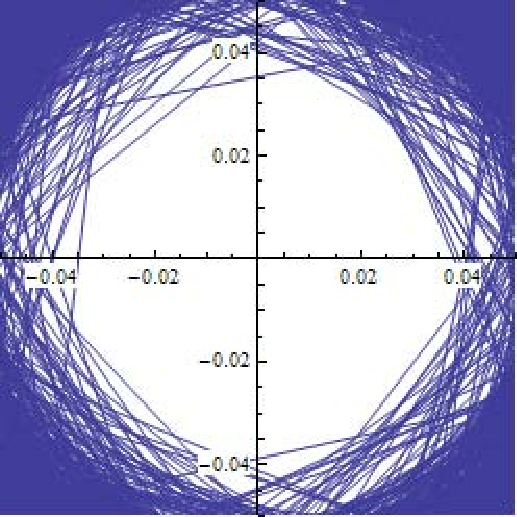
\includegraphics[width=0.32\textwidth]{CLEsmall-x1x2}%
~~~~~~~~
(b) %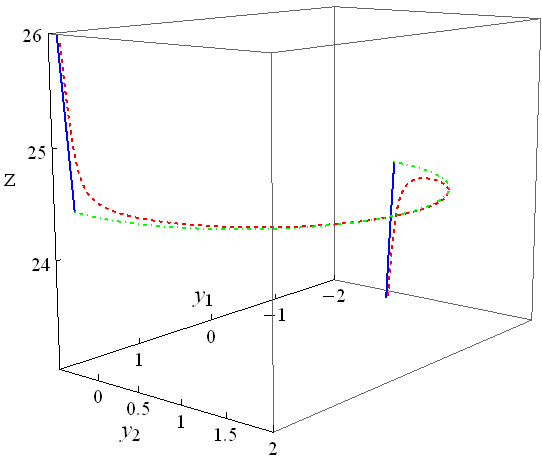
\includegraphics[width=0.42\textwidth]{singpass1}%
 \end{center}
 \caption{\label{fig:CLEsmall-x1x2}
A very long time ($t=5000$) simulation of \cLf. $\{x_1,x_2\}$ plot indicates
that probability of hitting $(x_1,x_2) =(0,0)$ is for all practical purposes
equal to zero, and $\sqrt{x_1^2+x_2^2} > 0.02$.
\hfill Predrag {Jul 14 2009}
%(The initial point is on the strange attractor).
}
\end{figure}
%%%%%%%%%%%%%%%%%%%%%%%%%%%%%%%%%%%%%%%%%%%%%

\item[2007-06-13 Predrag]
Learned nothing from Armbruster {\em et. al}: they showed that four
complex Fourier modes suffice to exhibit most of the qualitative features
of the dynamics, for a wide range of system sizes\rf{AGHks89}.

\item[2009-08-28 Predrag] Evangelos in his thesis and Kohler in his
\HREF{http://ChaosBook.org/projects} {ChaosBook.org project} got nothing
of interest out of Armbruster \etal\rf{AGHks89}.

\item[2012-03-26 Predrag]
There is Armbruster, Guckenheimer and Holmes\rf{AGHO288} flow with
$\On{2}$ symmetry:
\index{Armbruster-Guckenheimer-Holmes flow}
\beq
\begin{split}
  \dot{z}_1 &=\bar{z}_1 z_2
              + z_1\left(\mu_1+ e_{11}|z_1|^2+e_{12}|z_2|^2\right) \\
  \dot{z}_2 &=\pm z_1^2
              + z_2\left(\mu_2+ e_{21}|z_1|^2+e_{22}|z_2|^2\right)
  \label{eq:AGH}
\end{split}
\eeq
where $z_1,z_2\in \mathbf{C}$ and $\mu_j$ and $e_{jk}$ real parameters.
This system corresponds to the first few terms in the center manifold
reduction of a $\On{2}$-symmetric partial differential equation near a
codimension two bifurcation. It is a 2-mode system, so group orbits are
more interesting than for \cLf.
{\bf [2009-08-28 Predrag]} Evangelos in his thesis and
\HREF{http://chaosbook.org/projects/index.shtml\#Kohler}{Kohler} in his
\HREF{http://ChaosBook.org/projects}
     {ChaosBook.org project}
got nothing of interest out of Armbruster \etal\rf{AGHO288}. As far as we
can tell, it exhibits no chaos. I would prefer some modification of it
with $\SOn{2}$ symmetry only, and exhibiting chaos (done! see 2012-03-27
remark below). Or some version of 2-mode model Daniel has been playing
with which does not behave singularly. He has an unstable cycle close to
the origin that maybe does the trick.


\item[2012-03-26 Daniel] \refRef{PoKno05} and two others may provide some
candidate systems. Haven't had time to enter them into siminos.bib or
read through them but the look promising.

\item[2012-03-27 Predrag to Keith]
Porter and Knobloch\rf{PoKno05}
(\HREF{http://ChaosBook.org/library/PoKno05.pdf}{click here})
write: ``Chossat\rf{Choss93} has shown that breaking the symmetry
$\On{2}$ down to $\SOn{2}$ through the addition of small terms that break
reflection symmetry generically destroys the heteroclinic cycles and
replaces them by a quasiperiodic orbit characterized by two small
frequencies, one associated with the broken heteroclinic connection and
one with a slow drift along the group orbit of translations. Ashwin
\etal\rf{AshBoMe96} showed that this perturbation must be dispersive: if
reflection symmetry is broken by adding a constant through flow the cycle
will persist.''

This shows us how to get an $\SOn{2}$-equivariant model rather than
the Armbruster, Guckenheimer and Holmes\rf{AGHO288}:
``When the reflection symmetry is broken, the coefficients in the normal
form equations are no longer forced to be real and hence can be expected
to acquire imaginary parts'', their Eq. (10). Play with that one.

\item[2012-03-28 Daniel]                        \toCB
It is not the ``embedded template'' used in the topological theory of low
dimensional chaos. In Predrag's words, ``It is not THAT template''.

\item[2012-03-28 Daniel]
   The writing abruptly jumps from goody-goody intro for the everyman to
   technical without sufficient warning. Need to segway into the group
   theory stuff. UPDATE 2012-04-10: Definitely improved at this point

\item[2012-03-28 Daniel]
Rodriguez and Schell\rf{Rodriguez1990} may actually be a good system.
They are using a truncation of the Ginsberg-Landau equation, which
results in a 4D system of ODE's. These equations have parameters regimes
that are chaotic (as reported by Rodriguez and Schell and at least one
other researcher). They are $\SOn{2}$-equivariant. They only have a small
number of parameters (3). The truncation is a two-mode truncation so it
should provide more interesting group orbits than the one-mode Complex
Lorenz system.

``Within the two-mode approximation, and using
the transformation
\[ a_k = (b_k, c_k) = b_k + ic_k = r_k e^{i\theta_k}\,, \]
the LG equation reduces
to a set of four ordinary differential equations
for the variables $r_0$, $r_1$, $\theta_0$, $\theta_1$; however, it is more convenient
to replace the last two variables with the linear
combinations $\psi_1 = \theta_1 -\theta_0$, which is a phase
difference, and $\zeta = \theta_1 +\theta_0$, which is a phase sum.
''

\end{description}
Their system of equations is:
\index{Rodriguez and Schell flow}
\beq
\begin{split}
  \dot{r}_o &= \rho r_0\left( 1 - r_o^2\right)
                - r_0 r_1^2\left(\rho + \frac{1}{2}\rho\,\cos(2 \pi \psi_1)
                + \frac{1}{2} \sin(2 \pi \psi_1)\right) \\
  \dot{r}_1 &= (\rho - q^2 c_0)r_1 - \frac{3}{4}r_1^3 - r_1 r_0^2 \left(2 \rho
               + \rho\,\cos(2 \pi \psi_1) - \sin(2 \pi \psi_1)\right) \\
  \dot{\psi_1} &= \left[-2 q^2 + 2 r_0^2
                  - \frac{1}{2}r_1^2 +(2 r_0^2 - r_1^2)\,\cos(2 \pi \psi_1)
                  +\rho\,(2 r_0^2 + r_1^2)\,\sin(2 \pi \psi_1)\right]/2\pi
  \label{eq:RSsystem}
\end{split}
\eeq
\beq
  \dot{\zeta} = \left[-2 q^2 + 6 r_0^2
                  + \frac{7}{2}r_1^2 +(2 r_0^2 + r_1^2)\,\cos(2 \pi \psi_1)
                  +\rho\,(2 r_0^2 - r_1^2)\,\sin(2 \pi \psi_1)\right]/2\pi
  \label{eq:RSsysSum}
\eeq

At least two chaotic regimes are reported for this system. These occur
for $c_0 = \rho = 0.25$ and $q < 0.9787$ or $1.029039 < q < 1.029041$.

\begin{description}

\item[2012-03-28 Predrag]
notes on Rodr\'iguez, J. D. and Schell\rf{Rodriguez1990}.
What baffles me is that there are no ratios of form $r_0/r_1$ in
\refeq{eq:RSsystem}. In contrast, Daniel 2012-03-13 derived for the
2-mode system in ChaosBook the polar coordinates form
\bea
   \dot{r}_1 &=& -\sigma r_1 + \sigma r_1 r_2 \cos(\theta)\continue
   \dot{r}_2 &=& -r_2 + r_1^2 ((\rho_1 - z) \cos(\theta) - \rho_2 \sin(\theta))\continue
   \dot{\theta}_1 &=&  -\sigma r_2 \sin(\theta)\,,\quad
   \dot{\theta}_2  =  -e + \frac{r_1^2}{r_2} ((\rho_1 -z) \sin(\theta)
                       + \rho_2 \cos(\theta))\continue
   \dot{z} &=& -b z + \frac{r_1^2}{r_2} \cos(\theta)
\,,
\label{eq:2meRpol}
\eea
where $\theta = 2 \theta_1 - \theta_2$, and
rewriting the angular part as $\dot{\theta} = 2 \dot{\theta_1} - \dot{\theta_2}$,
\beq
\dot{\theta} = e - \frac{r_1^2}{r_2} ( (\rho_1- z) \sin(\theta)+\rho_2 \cos(\theta))
- 2 r_2 \sigma \sin(\theta)
\ee{eq:2meRangl}
Simulation of these equations (as well as of \cLe\ in polar coordinates
and Dangelmayr and Armbruster, Guckenheimer and
Holmes \refeq{eq:AGpolar} below)
runs into both $r_j= 0$ singularities, while \refeq{eq:RSsystem} seems to
have none. What gives?

\item[2012-03-31 Predrag]
``[...] we consider a subclass of systems with circular symmetry: those
invariant under the rotations in the plane, i.e., operations of
the symmetry group $\SOn{2}$\rf{golubII}.'                                  \toCB
[...] We show that even though phase locking cannot occur in systems with
rotational symmetry, the locking of phase differences does occur.''
[...] we have also discovered one exception in the
correspondence found in the previous investigation.
[...] There exists a small interval between the regions of quasiperiodic
behavior ($\Delta q < 10^{-6} $) in which chaos occurs. Although we were
unable to locate this asymptotic chaos in the appropriate parameter range
of the LG equation, we did observe ``transient chaos''.

[...] it can be verified by substitution that phase
differences, which are defined as
\(
\psi_1 = (\theta_1-\theta_0)/\pi \,,\;
\cdots\,,
\psi_j = (\theta_j-\theta_0)/\pi \,,\;
\cdots\,,
\)
can become fixed and are represented in a subspace by the fixed points,
$\psi =$ constant, $r_0= 1$, $r_j= 0$, where $j= 1,2,\dots$.

[Predrag: why would they want to lock? The  locking the study happens
prior to bifurcations to chaos, I do not think we care. What is the point
of looking at all $r_j= 0$ ?]

``[...] It may seem somewhat strange to speak of a locked phase
difference between two modes, when one of the modes has zero amplitude.
However the quantity $\theta_1$ is rigorously defined as the phase of a
Fourier component whose amplitude asymptotically decays to zero and
hence, the locked phase difference is well defined as an asymptotic limit
for the phase difference.''

\item[2012-03-31 Predrag] Stopped studying their 2-mode equations here,
not sure it's what we want to use...

\item[2012-03-28 Daniel]
At first, glance it seems like Mercader and Prat\rf{MePrKn01} might
be a candidate if we decide to go with $\On{2}$ symmetry since really the
Rayleigh-Benard problem has $\On{2} \times Z_2$ symmetry and they are really
talking about breaking the $Z_2$ part. They have a reduced model, but I'm
not sure that it is chaotic.

\item[2012-03-31 Predrag]
notes on Mercader and Prat\rf{MePrKn01}.
\index{Armbruster-Guckenheimer-Holmes flow}
The effects of weak breaking of the midplane reflection symmetry on the
1:2 steady state mode interaction in Rayleigh�B\'enard convection are
discussed, with bifurcations galore, ala Knobloch. They do it for the
full PDEs, but in Sect.~4 motivate results by discussing them in the
context of $\On{2}$-equivariant amplitude equations for 1:2 mode
interactions.
We note that the Dangelmayr\rf{Dang86} and Armbruster, Guckenheimer and
Holmes\rf{AGHO288} third order in the amplitudes normal form flow with
$\On{2}$ symmetry \refeq{eq:AGH} does have ratios of form $r_0/r_1$, when
rewritten in the polar form (Eq.~(4) in the paper),
\bea
   \dot{r}_1 &=& \mu_1 r_1 + a_1 r_1^3  + b_1 r_1 r_2^2
                 + c_1 r_1 r_2 \cos(\psi)\continue
   \dot{r}_2 &=& \mu_2 r_2 + a_2 r_1^2 r_2  + b_2 r_2^3
                 + c_2 r_1^2 \cos(\psi)\continue
   \dot{\theta}_1 &=&  - c_1 r_2 \sin(\psi)\,,\quad
   \dot{\theta}_2 = -e_2 + c_2 \frac{r_1^2}{r_2} \sin(\psi)
\,,
\label{eq:AGpolar}
\eea
where $\psi = 2 \theta_1 - \theta_2$, and Predrag stuck in tentatively an
`$e_2$' term because something like that is needed to break $\On{2} \to
\SOn{2}$. Rewriting the angular part as $\dot{\psi} = 2 \dot{\theta_1} -
\dot{\theta_2}$:
\beq
\dot{\psi} = e_2 - \left(c_2 \frac{r_1^2}{r_2} + 2\,c_1 r_2\right) \sin(\psi)
\,.
\ee{eq:AGphase}
The equations possess pure $n = 2$ solutions but no pure $n = 1$
solutions (except for the discrete `midplane reflection' symmetry
invariant subspace?). Most solutions are `mixed modes'. I do not think we
care about the `midplane reflection' symmetry (with 5th order normal
form), so we only need \refeq{eq:AGpolar} to determine the \reqva.

\item[2012-03-28, 2012-03-31 Predrag] I'm still in favor of trying {\bf
[2012-03-27 Predrag]} Porter and Knobloch\rf{PoKno05} above, as I prefer
the most cited model. The exact 1:2 resonance ODE normal form was
treated first by  Dangelmayr\rf{Dang86} and analyzed by the more cited
Armbruster, Guckenheimer and Holmes\rf{AGHO288} and Jones and
Proctor\rf{JoPro87} (for a  general reference containing this material,
see Golubitsky \etal\rf{golubII}, ch. XX, section 1), and keeps getting
cited a lot\rf{AshDang05,PoKno05,SmMoehHo05}.

Making it $\SOn{2}$-equivariant is easy, just make a coefficient complex
- I have forgotten, but that's how we got to the \cLe. If the imaginary
part is small, then you turn orbits that used to be \po s into \rpo s.
That's why {\bf [2012-03-22 Bryce]} \rpo s were nearly periodic. But
truncations of the Ginsberg-Landau equation have their market too.

Play with them both, we pick one eventually that illustrates multiple
charts better.

\item[2012-03-28 Daniel]
Is there a way for us to upload papers into the Chaosbook library and
would this be something that we should be doing?

\item[2012-03-28 Predrag] Read \refsect{s:HowToLit}.

\item[2012-03-28 Predrag] Despite of my worries that
large {\phaseVel} is a real effect, Daniel has constructed 2-chart
atlas of \cLe\ that looks pretty credible. Will be shown here.

\item[2012-03-29 Daniel] Figured out what was wrong with code.
\refFig{fig:sliced} illustrates the sliced attractor,
\reffig{fig:unsliced} the unsliced one. Have theater tickets, but will
blog later...

\item[2012-03-30 Keith] As discussed yesterday with the gang, got the
unstable manifold of R\"ossler going.  I will work on parameterizing later
today/tomorrow for a return map.  Also have been thinking about the two
chart atlas...I still wonder if there is an easier way to do the template
choice...I will think about this more.

\begin{figure}
\begin{center}
  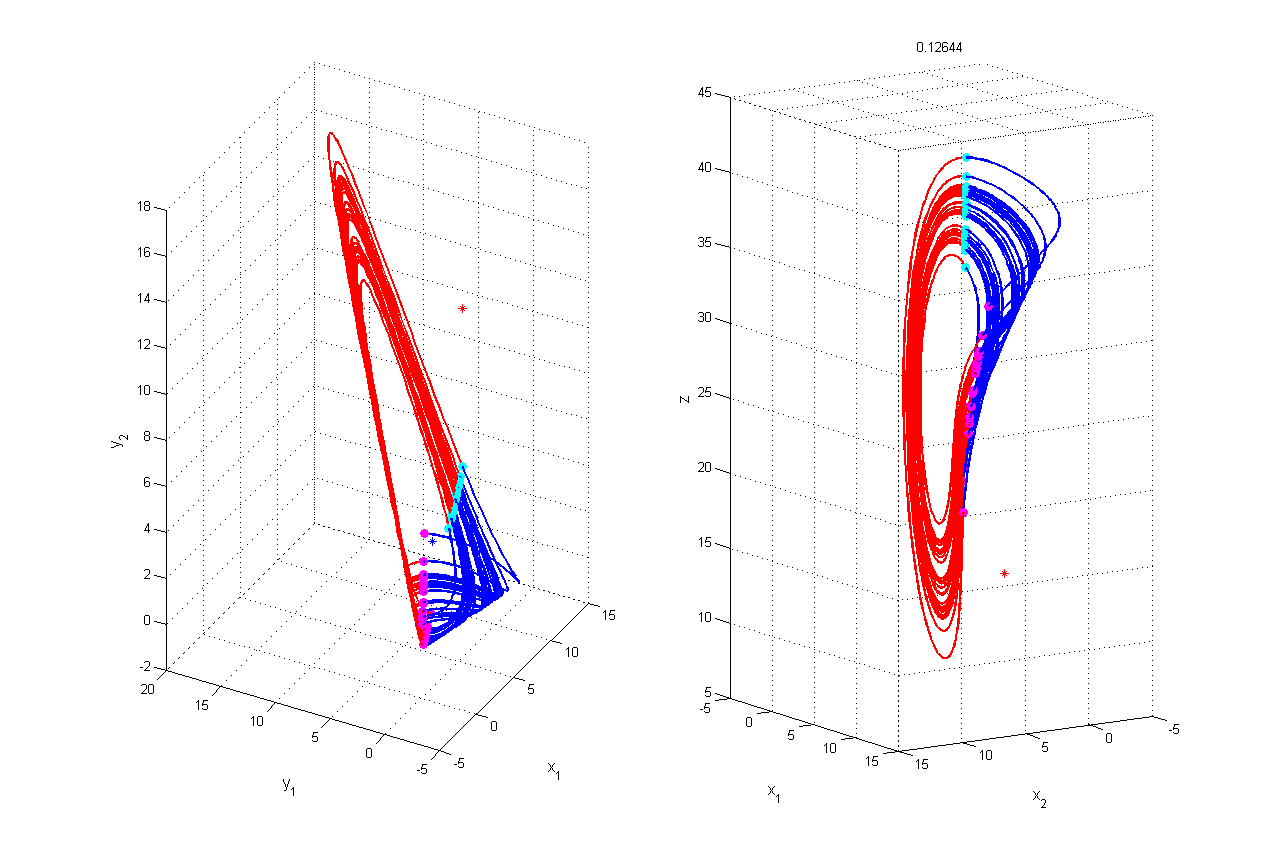
\includegraphics[width=0.6\textwidth,clip=true]{SLICED}
\end{center}
  \caption{
  Sliced attractor, switching between templates.}
\label{fig:sliced}
\end{figure}

\begin{figure}
\begin{center}
  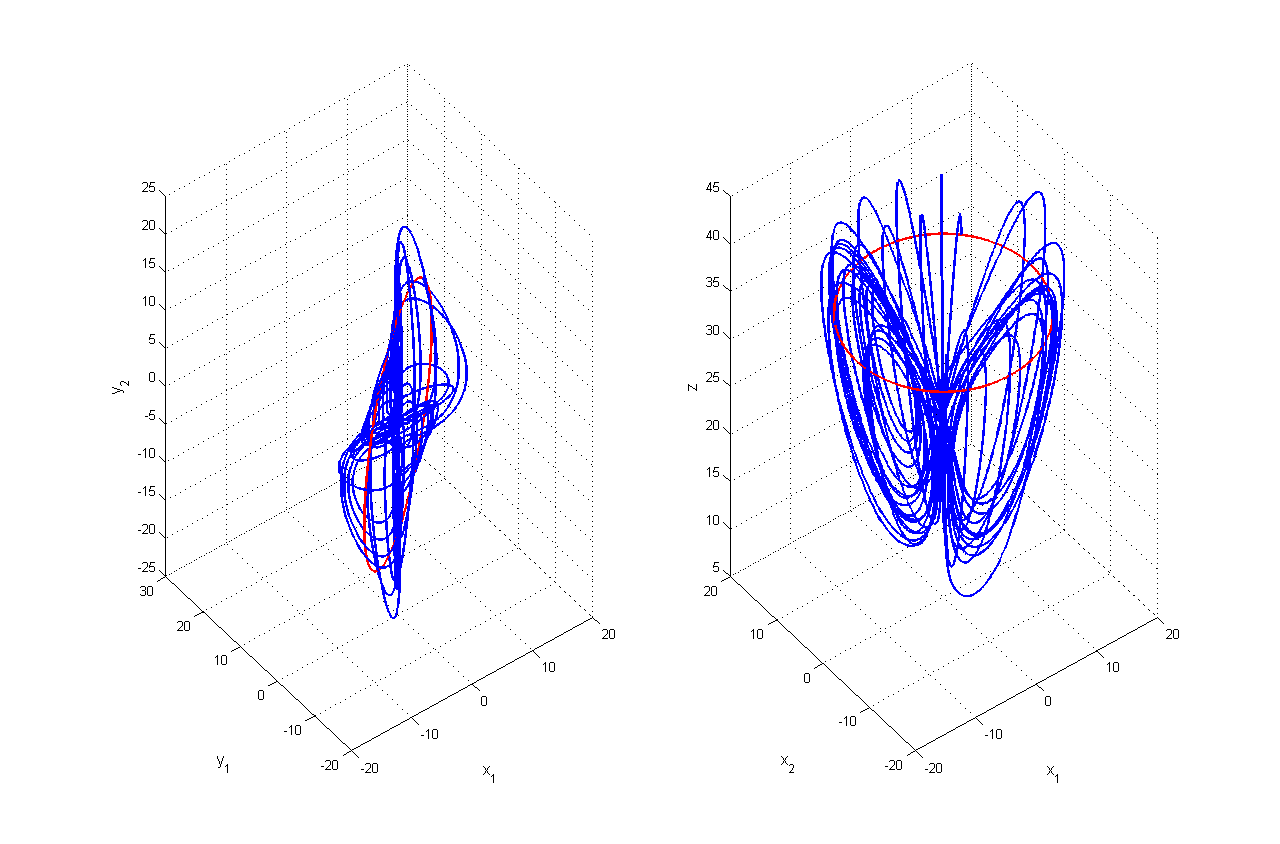
\includegraphics[width=0.6\textwidth,clip=true]{UNSLICED}
\end{center}
  \caption{
  Same trajectory in full space.}
\label{fig:unsliced}
\end{figure}


\item[2012-03-30 Daniel]
During our discussion yesterday Keith pointed out that while checking for
a sign change in
\[
\braket{(\sspRed(\zeit)- \slicep{}^{(2)})}{\sliceTan{}{}^{(2)}}
\,.
\]
makes sense, it really gets you nothing more than checking for a sign
change in the slice condition for $\sliceTan{}{}^{(2)}$ since
$\braket{\slicep{}^{(2)})}{\sliceTan{}{}^{(2)}} = 0$, anyway. At least
this is the case for SO(2) rotations... How generic is this? Should the
crossing condition be amended in the Chaos Gang paper?

\item[2012-03-31 Predrag] You are correct - have now fixed that in the
tex proper.

\item[2012-03-31 Keith] Still working on parameterizing the
curves/getting a return map.  If you fix the section you look at the
unstable map, should the return map look different?  Some thinking makes
me believe this is so, but am looking for input...Thinking of an idea for
finding two slices (instead of random guessing)...I'll play with the idea
for the next day or two.

\item[2012-03-31 Predrag] We do need a good algorithm for computing the
return map, now that the ridge Poincar\'e section of 2-chart Daniel's
slicing of \cLe\ looks so nice. If the description in ChaosBook is
unclear, be specific about what the problems are. Also
\HREF{http://chaosbook.org/projects/index.shtml\#Basu}
{Basu's project} and associated links might be useful.

Do not understand ``If you fix the section you look at the unstable
map,'' but: For each section the return map looks different. They are all
smooth conjugacies of each other, dynamically equivalent, but awkward
sections yield awkward return maps.

\item[2012-03-31 Predrag] The battle plan suggestion to ChaosGang:
\begin{itemize}
  \item
        Two of you finalize drawings and text for R\"ossler sections and
        their borders.
  \item
        One of you finalizes drawings and text for Daniel's 2-chart
        sliced \cLe\ (preferably not Daniel).
  \item
        One of you computes (presumably numerically) \reqva\ of the
        $\SOn{2}$-equivariant version of Dangelmayr 2-mode
        \refeq{eq:AGpolar}, and (hopefully) their \stabmat\ \Mvar\
        eigenvalues, plays with parameters. We would like the \reqva\ to
        be complex-pair unstable, leading to chaos, to be visualized and
        sliced in Cartesian coordinates \refeq{eq:AGH}.
\end{itemize}

\item[2012-04-01 Predrag] Small worry about Daniel's computer-optimized
2-chart atlases; It would be nicest if the same set of {\template s} did
double duty - be the {\template s} both for the sections and slices.
These choices unrelated to any invariant solutions ar not going to yield
nice sections in the sense of \reffig{fig:A29PoincBad}.

\item[2012-04-01 Predrag] Serious worry about multi-chart atlases:
pair-wise templates are in each other's slice, and the ridge between them
is rigid. But doubt this can be done for sets for three or more
{\template s} on a curve surface...

\item[2012-04-02 Daniel]
In case anybody was wondering how we
ere's how I got my two chart atlas for the
\cLe. At first, I tried using the
\reqv\ and various points on the $\cycle{01}$ relative
periodic orbit as templates. I could not get this to work as $\dot{\phi}$
always seemed to blow up to anywhere between 200 and 1500.
\emph{However}, I did check $\braket{\,t\,}{\sliceTan{}{}}$ as I went and
while it got small, it never quite switched signs, so technically it
never really crossed the template border. I guess the large values of
$\dot{\phi}$ probably had to do with the actual physical rotation induced
by the strong contraction toward the z-axis.

Since thinking didn't get me anywhere and it was 3 AM, I decided to just
compute. What I did was that I started with two templates (I believe one
was Fr\"olich's template from eq. \ref{exmplTempl}, for no particularly
good reason, and a point on $\cycle{01}$), I integrated the
$\cycle{01}$ orbit and calculated what the maximum of $|\dot{\phi}|$
was. I then wrote a loop that added some small random vector to each of
the templates, integrated the same orbit, and checked whether the max of
$|\dot{\phi}|$ got smaller or bigger. If it got smaller, I kept those two
new templates and started adding noise to them. I let this run over night
and ended up with the following two templates, which gave me a max
$|\dot{\phi}| \sim 16$ for the $\cycle{01}$ orbit and $\sim 25$ for an
ergodic trajectory:

$\slicep{}^{(1)} = [10.6826557605063, 4.05746018793401, 3.86638880437299, 9.62155656768089, 33.3136330008352]$ \\

$\slicep{}^{(2)} = [90.4054673767747, 22.7146855264444, 31.5729216223112, 110.683144276042, 112.538644670233]$\\

The reason that the second one is so big is that I accidentally used the
rand function in Matlab instead of randn, so the code was only adding
positive numbers to the original point. That being said, this can be
partially fixed by rescaling and adjusting the z value to whatever is
convenient. This can be done because the only way that the templates come
into the computation is through their group tangents, which always has a
zero z-component. Rescaling is possible because the group tangent vector
of the template only comes in for orthogonality checks
$\braket{\,t\,}{\sliceTan{}{}} = 0$ or in the calculation of
$\dot{\phi}$, where it is in both the numerator and the denominator. The
magnitude of the tangent does not matter in either of these cases. Still
it is kind of worrisome that one can't (or at least I haven't been able
to) pick something intelligently, and that these points are not really
that close to the attractor.

One final note... While I did the template switching and this this looks
good, the trajectories look good if you use just \emph{one} of these
templates and the max of $|\dot{\phi}|$ isn't much bigger.

\item[2012-04-03 Predrag to Daniel] It seems fixing a template amounts only to defining a ray in the
$2 + 2$-dimensional $m=1$ subspace, the only object that matters for charts, borders, ridges is
\bea
\sliceTan{}{}^{(1)} &=& c_1 (4.05746018793401, -10.6826557605063,  9.62155656768089, -3.86638880437299, 0)
    \continue
\sliceTan{}{}^{(2)} &=& c_2 (22.7146855264444, -90.4054673767747, 110.683144276042, -31.5729216223112, 0)
\,,
\label{DanielTmpls}
\eea
with $c_1$ and $c_2$ arbitrary factors. You can chose them so
$\sliceTan{}{}^{(j)}$ are unit vectors, if you wish. Can you look for
minima of
$1-\groupTan{\sspRed{\zeit}} \cdot \sliceTan{}{}^{(j)}
   / \Norm{\groupTan{\sspRed{\zeit}}} \Norm{\sliceTan{}{}^{(j)}}$, $\sspRed{0} \in \pS_{110}$?
Maybe then you could move the \template\ onto the cycle; it would be
nicer if the templates were on invariant solutions... Better still, find
parameter values for which the 2-chart atlas for 2-mode system is a
better example than this.

\item[2012-04-02 Evangelos to Daniel] Did you use some kind of end condition in
your loop or is this just what you got after many iterations? I try to understand
whether you could get more template points with similar $\max |\dot{\phi}|$.
I wonder if there is any variational principle that could drive the search of
a good set of template points.
Also, it would be interesting to plot the trajectories in each of the two slices.

\item[2012-04-03 Evangelos]
In \refref{SiCvi10} I've tried to avoid singularities by modifying the
template point in a way that seemed intuitive to me back then (that I was immersed
into the problem) and I don't understand anymore. I claim that if we pick a template
with larger $y_2/y_1$ than the \reqv\ we can avoid
the singularity. See Sec. 6.3 and Fig 7(b).
(There is a discrepancy between what I plot in the figure and what I say in the
text, which I think is due to an inconsistency in rotating and rescaling the
template and should not be essential).

\item[2012-04-03 Predrag to Evangelos] We have learned several important things since
2010.
\begin{enumerate}
  \item
    please study and either understand \chartBord s and ridges, or show
    why the construction is wrong. A chart \emph{is not} the hyperplane,
    it is flat tile carved out of the hyperplane that \emph{by construction}
    slices group orbits in template's neighborhood \emph{only once}.
  \item
    it appears that the \cLe\ strange attractor we are studying never
    gets as far as the \chartBord\ (where \refeq{sliceSingl0} changes
    sign) but only gets squished close to the $z$-axis, with
    \refeq{sliceSingl0} maintaining sign. So there is a dynamical reason
    for large $\dot{\gSpace}$ which is not an artifact of slicing. That's
    not what we are trying to illustrate here. That is why I keep
    suggesting that Gang of Chaos constructs a more interesting 2-chart
    atlas for 2-mode systems such as \refeq{eq:AGH} and\refeq{eq:AGpolar}.
\end{enumerate}


\item[2012-04-02 Keith] Have working return map for the
R\"ossler, \reffig{fig:RoessRetMap}.  I will post the code
when I clean it up and comment it; it is too Keith-cluttered currently.
Does anyone know how to put an \"o into matlab titles/strings?

\item[2012-04-03 Predrag to Keith] You do not want to insert text like
'R\"ossler blah blah' into figures; that belongs to the caption. Keep
figures lean, clean and mean.

\begin{figure}
\begin{center}
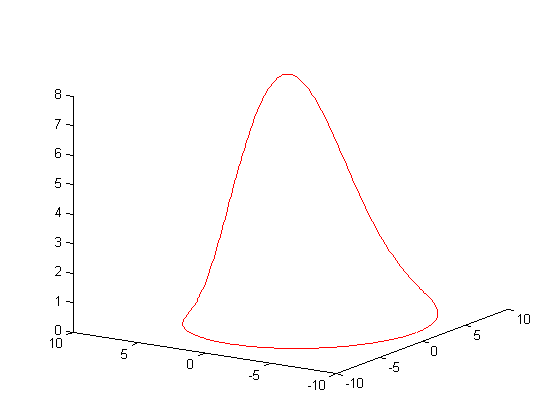
\includegraphics[width=0.6\textwidth,clip=true]{Rossler1Period}
\end{center}
  \caption{
R\"ossler \po\ \cycle{1}.
  }
\label{fig:Ros1Per}
\end{figure}

\item[2012-04-03 Predrag] Presumably \reffig{fig:RoessRetMap} is obtained
by starting close to the \eqv\ $\EQV{0}$ and then indicating the
Poincar\'e section returns, iterating so long enough that you start
filling out the strange attractor. You want to draw instead the unstable
manifold of $\EQV{0}$ up to the turnback, as a line.

\item[2012-04-03 Daniel to Evangelos]
It was not a particularly smart way to go about it. I just took a set of
templates, ran a simulation of one period of $\cycle{01}$ (calculated
on the slices as per \refeq{reconstrEq} and \refeq{EqMotMFrame}  and
switching from $\hat{x}^{(1)}$ to $\hat{x}^{(2)}$ whenever necessary as
per \refeq{eq:chartBord}), calculated $\max |\dot{\phi}|$ for the time
series, and figured out whether it was smaller or larger. If it was
better, I saved it as my new ``standard'' to compare to. The next
calculation started with the best templates so far plus some noise. I
just let it run until the morning and saw what the best one that it had
found was. There is no guarantees that the are the best. They are just
the best that the dumb algorithm found. There are other templates (beyond
the rescaling that Predrag mentioned above) that work similarly.

\item[2012-04-03 Daniel to Keith] I agree with Predrag leave titles and
such out of the figure and just caption it. However, you can do it by
\begin{verbatim}
title('R\"ossler','Interpreter','latex')}
\end{verbatim}
or by just putting in the \"o directly (as in using the
ASCII character for it). This may require you to use escape sequences
(ALT + \#) or configure your keyboard differently.

\item[2012-04-03 Daniel to Predrag] I played around with the parameters
in \refeq{eq:AGpolar} all afternoon and couldn't find anything chaotic.
Everything was either attractive fixed points or periodic orbits, which I
guess are relative equilibria/periodic orbits, since the symmetry is
quotiented out by going to polar coordinates. I guess I'll turn to the
literature to see if somebody has a set of parameters where they see
chaos...

\item[2012-04-03 Predrag to Lei]
We have to move on with ChaosGang paper. Please follow ChaosBook
teachings on how to analyze a dynamical system (it is not by blindly
simulating):
\begin{enumerate}
  \item
        determine \emph{numerically} the \reqva\ of the
        $\SOn{2}$-equivariant Dangelmayr 2-mode system in polar coordinates
\bea
   0 &=&  r_1 (\mu_1 + a_1 r_1^2  + b_1 r_1 r_2
                 + c_1 r_2 \cos(\psi))  \continue
   0 &=& \mu_2 r_2 + a_2 r_1^2 r_2  + b_2 r_2^3
                 + c_2 r_1^2 \cos(\psi)\continue
   0 &=&  e - \left(c_2 \frac{r_1^2}{r_2} + 2\,c_1 r_2\right) \sin(\psi)
\,,
\label{eq:AGpolarREQV}
\eea
        Here I stuck in tentatively an `$e$' term because something like
        that is needed to break $\On{2} \to \SOn{2}$, verify that it
        really does that. The first two equations are cubic, the third one you can use
        to eliminate $\cos(\psi)$, so my guess is that there could  be up to six real
        roots, but I have not thought it through. Once you have found parameters
        for which there are interesting \reqv\ solutions, then
  \item
        compute analytically the \stabmat\ \Mvar\ in polar coordinates
  \item
        Study eigenvalues, keep playing with parameters. We would like
        -preferably- no \reqv\ to be attracting limit cycle, and several of
        the \reqva\ to be complex-pair unstable, leading to chaos, to be
        visualized and sliced in Cartesian coordinates \refeq{eq:AGH}.
  \item
        If you find a nice chaotic attractors, others can join in
        constructing an atlas for it. We just need one and only one
        example with non-trivial \chartBord s and at least 2 charts.
\end{enumerate}
Please read the blog entries above, my writing is starting to get a bit
repetitive - a look at
\HREF{http://chaosbook.org/projects/index.shtml\#Kohler}{Kohler} in his
\HREF{http://ChaosBook.org/projects}{ChaosBook.org project} might be
helpful, but we \emph{do not} want to study $\On{2}$ discrete symmetry
invariant subspaces. The papers discussed above exhibit some stable \reqv
a and \rpo s for specific (out-of the hat) parameter choices. You want to
screw up some parameters higher so these solutions go unstable.

\item[2012-04-05 Lei to Predrag]
I can see the $e$ added really breaks the $O(2)$ symmetry to $SO(2)$
symmetry. As rotations don't change the equations and reflections change
the sign of the last equation, adding a nonzero $e$ will break the
reflection symmetry.

By eliminating $\psi$, I got two polynomial equations of order 10. So
there are 20 complex solutions. I tried parameters $\mu_1=\mu_2=-1$,
$a_1=a_2=b_1=b_2=c_1=c_2=1$, and got 8 real solutions. All the 8
solutions I got for $(r_1,r_2)$ are $(\pm 0.537655,\pm 0.537655)$ and
$(\pm 0.980269,\pm 0.980269)$. In this case, 6 equilibria points have
only real eigenvalues, two equilibria points have complex eigenvalues
with positive real parts. Will this case work? Others please check
whether the calculation is correct or not.

\item[2012-04-05 Keith to Lei]
Lei what was your $e$ value?

\item[2012-04-06 Predrag to Lei] By definition, $r_i \geq 0$, so you have
only two roots: $(0.537655,0.537655)$ and $(0.980269,0.980269)$. I find
it surprising that $r_1=r_2$, as equations look asymmetric in $r_i$;
might be consequence of $a_1=a_2=b_1=b_2=c_1=c_2=1$ (what value $e$? also
$e=1$?), you want to break this artificial symmetry if it is the cause. If
$r=r_1=r_2$ you have
\bea
   0 &=&  r (\mu_1 + (a_1 + b_1) r^2
                 + c_1 r \cos(\psi))  \continue
   0 &=& r (\mu_2 + (a_2 + b_2)  r^2
                 + c_2 r \cos(\psi))\continue
   0 &=&  e - r \left(c_2 + 2\,c_1\right) \sin(\psi)
\,,
\label{eq:AGpolarR1R2}
\eea
which looks degenerate for your coefficient values.
There is an \eqv\ for $r_1=r_2=0$. There is a subspace $r_1=0$, $r_2 > 0$
which you can solve analytically - it my cause us some trouble. If what
you end up solving is a polynomial in $r_1$, you want to divide it with
all these known roots, see whether anything of interest is still left.

Keep fishing...

\item[2012-04-06 Keith]
Met with a bunch of people today (Sarah, Luis and Bryce).  Sarah and Luis
didn't get to stay too long, but we worked on the R\"ossler 2 section
problem.  Bryce has the results of the meeting and should be posting them
later today.  We managed to find two planes that cut the rotations at
both {\eqv} and the ridge distance looks like it might be minimized
between the {\eqv}.  The problem is that we are having a difficult
time understanding how the mapping will work fit together.  We also tried
playing with how the {\poincBord} looked on both planes.

\item[2012-04-06 Daniel]
Have been working on visualizing group orbits and such.
\refFig{fig:CLf01group}\,(b) is an updated version of \reffig{fig:CLERPO001}
but for $\cycle{01}$ instead of $\cycle{001}$. Thoughts? Comments?
If people think this looks good, I'll update the code that generated it.

Also, I guess I forgot to mention this earlier when I blogged about
constructing the 2-chart atlas. If one does not carefully track the
crossing of the ridge, funny things can happen, unless you are careful.
Suppose you start computing on slice 1 and detect a ridge crossing. This
means you now need to start computing on slice 2. If you don't track the
crossing exactly, you end up using a point that is on slice 1 and very
close to but not on slice 2. This gives you slight error in your
calculation on slice 2 which the calculation quickly irons out. However,
sometimes when the code rotates the point into slice 2, it quickly
changes the sign on the ridge crossing condition into slice 1. This shows
up as two quick crossings between templates (one time step apart) and
ends up looking like the trajectory on the two templates get mixed. This
can be fixed by checking the direction of the crossing of the ridge
rather than for just a simple sign change. See \reffig{fig:2chartfail},
as opposed to  \reffig{fig:sliced} for an example of this.

\begin{figure}
\begin{center}
  \includegraphics[width=0.6\textwidth,clip=true] %,height=0.5\textheight
  {2chartfail}
\end{center}
  \caption{ If one is not careful about monitoring ridge crossings, you
  can end up with a situation where both templates are used on both sides
  of the ridge}
\label{fig:2chartfail}
\end{figure}

\item[2012-04-07 Predrag to Daniel] Your \reffig{fig:CLf01group}\,(b) is
fabulous, I moved it to the article draft.

\item[2012-04-06 Bryce]  The Chaos gang, as Keith mentioned in his
previous blog post, sat down to address the 2 section scheme for the
R\"ossler system. The condition that Predrag suggested, namely
minimizing the distance between the ridge and the two {\eqv}
points, was achieved in the following manner. Each section was
constrained to contain the unstable eigen-directinos but allowed to
rotate about that eigenvector. Each normal vector was then constrained by
rotating it about its respective unstable eigen-direction and assigning
this rotation angle a unique value, say $\theta$ or $\phi$. We notice
that as we rotate the two planes the dot product between them changes. In
particular, we seek the dot product between the two $\hat{n}$ that is
minimized which should simultaneously satisfy the condition that the
distance between the ridge and the two {\eqv} will be minimized. The
problem is now reduced to solving a system of two equations with two
unknowns:
\[
\partial_{\phi}(\hat{n}_1\cdot\hat{n}_2)=0,\, \partial_{\theta}(\hat{n}_1\cdot\hat{n}_2)=0
\,.
\]
My software of choice in plotting the two sections has been Mathematica
while Keith is using Matlab. Our results are indeed consistent but it is
up for debate as to how we want to present our results graphically. The
images shown below clearly demonstrate the {\poincBord s}
indicated by the color transitions between green and red and visa versa.
The brown line defines the ridge between the two sections while the blue
arrows indicate the unstable eigen directions at each \eqv\ point.

\item[2012-04-07 Predrag to Bryce] I moved \reffig{fig:RoessSct1}, to the
article draft. They look good to me, but will need some more twirling
around. Not publication quality yet, so blog their progress in
\refsect{s:figsToDo}.

\item[2012-04-06 Bryce to Sarah]
you mentioned that you have the equations for the conic sections.
If you look carefully at my plots you'll see that I have discretized the
planes into a bunch of points. If we utilized  your analytic equations
for the sections we could greatly improve the look and feel of the plots.
If your equations are in terms of the $\hat{n}$ vector defining the
sections and a general template point then implementing the sections
should be trivial.

\item[2012-03-16, 2012-04-07 Predrag to Sarah] see my {\bf [2012-03-11]}
post above, that wiki seems to say all we need to define a conic section
for R\"ossler $\{\dot{x},\dot{y},\dot{z}\}$, in $\{x,y,z\}$ coordinates.

\item[2012-04-10 Lei to Predrag] I've been played with the parameters of
the 2-mode system for a while. What I did is simply randomly chosen all
the parameters and see what kinds of eigenvalues we can get. Under the
condition $r_1$ and $r_2$ being nonnegative real numbers, it seems that I
always got two equilibria points. One possible set of parameters I found
may be of interest are
$\mu_1=-1,\mu_2=-4,a_1=1,a_2=1.5,b_1=3,b_2=2.5,c_1=3,c_2=3.5,e=0.1$. The
equilibria points are $(r_1,r_2)=(0.0516508, 1.26311)$ and
$(0.467095,0.2146)$. The corresponding eigenvalues are
$(19.9398,0.8495,-11.9818)$ and $(1.5352,-4.7992+0.0327i,
-4.7992-0.0327i)$

\item[2012-04-10 Predrag to Lei] I think we need $\psi$ as well, \ie,
\begin{itemize}
  \item $\REQV{}{1} = (r_1,r_2,\psi)=(0.0516508, 1.26311,?)$ and
        $\REQV{}{2} = (0.467095,0.2146,?)$
  \item their plots in the Cartesian coordinates
  \item $\dot{\theta}$ to see how slow/fast are they. $\dot{\theta}$
        might be related to 4th eigenvalue, when you go back
        to Cartesian coordinates
  \item stability eigenvalues, eigenvectors of the \eqv\ $\EQV{0}$ at
        origin, at your parameter values - if it is stable, everything
        just might fall into it and die.
  \item plots of small perturbations of the above \eqv\ and \reqva\ in
        the Cartesian coordinates to see whether the dynamics looks
        chaotic
  \item $\REQV{}{1}$: 2 large positive eigenvalues looks scary - probably
        nothing re-visits this \reqv. A mildly unstable complex pair
        would have been sweeter. You get complex eigenvalue by Hopf-bifurcating off a
        stable orbit, typically.
  \item $\REQV{}{1}$: Does either unstable eigenvalue become a complex
        eigenvalue pair in Cartesian coordinates?
  \item $\REQV{}{2}$: contracting eigenvalues have very small imaginary
        part, so the presumably just rocket toward the \reqv, not much
        spiraling there. At least the unstable eigenvalue seems slow
        compared to all other eigenvalues.
  \item $\REQV{}{1}$: Does the unstable eigenvalue become a complex
        eigenvalue pair in Cartesian coordinates?
\end{itemize}


\item[2012-04-10 Lei to Bryce] Maybe just some easy calculation, but I
don't get it. Why can we reduce the problem of minimizing the distance
between the ridge and the two equilibrium points to the problem of
minimizing dot product of normal vectors?

\item[2012-04-10 Bryce] Updated the plane rotation code on Dropbox. Lines
are commented and cleaned up for easier manipulation.

\item[2012-04-10 Bryce to Lei] The approach Keith and I took was more of
a ``gutsy'' feeling more than anything. A rigorous mathematical proof
isn't in our hands but I posted code on dropbox titled ``plane
rotation.nb'' that you can mess with to get a better feel for how the
distance between the ridge and two equilibrium is minimized by minimizing
the dot product between the two planes.

\item[2012-04-10 Predrag to C Gang]
Please focus on producing the 4 R\"ossler figures in the publication quality NOW.
It takes time - we can improve them later, while we wait for the referee report.

\item[2012-04-10 Predrag to Daniel]
Please focus on producing the 4 \cLe\ figures in the publication quality NOW.
It takes time - we can improve them later, while we wait for the referee report.
That one might ask us for lots of extra hoops...

\item[2012-04-10 Daniel] Are we using $S$ or ${\cal S}$ as the variable
for the section border? Both are used in the text.
{\bf Predrag:} ${\cal S}$ is more consistent with $\pS$ and $\PoincS$
notation.

\item[2012-04-10 Daniel] I thought the method of slices was not in
everybody's bag of tricks. We also discuss some further methods, at least
as per the outline. Predrag: agreed.

\item[2012-04-10 Predrag to Keith] Thanks for correcting
\refeq{eq:Rossler} - now I wonder where did I clip the wrong equation
from? Perplexing...

\item[2012-04-10 Bryce to Gang] After poking around in Mathematica for
some time I have resolved a much better method for plotting the sections
for R\"ossler flow along with the ridge, orbit, etc... Stripping the
points off of my current plots I can produce surfaces which will really
smooth out things. There was also no need to discretize the {\poincBord
s} as we have $\hat{n}$ along with the equations of the plane and the
equations of motion which reduces the contraint for the {\poincBord} to
one variable. Extracting the analytical equation and plotting the results
will be the task for later this evening.

\item[2012-04-10 Keith] Worked with Bryce to get R\"ossler figures.  He
is working with mathematica and I am with matlab; he is going to post his
results as well.  Here is some of the recent plots I have for the 4
R\"ossler pictures.  I am interested in feedback about what needs to be
done/added/etc.  I can manipulate the code as needed but matlab takes
some time.  See \reffig{fig:neareq} and \reffig{fig:twoplane}.

 \begin{figure}[H]
 \begin{center}
%(a)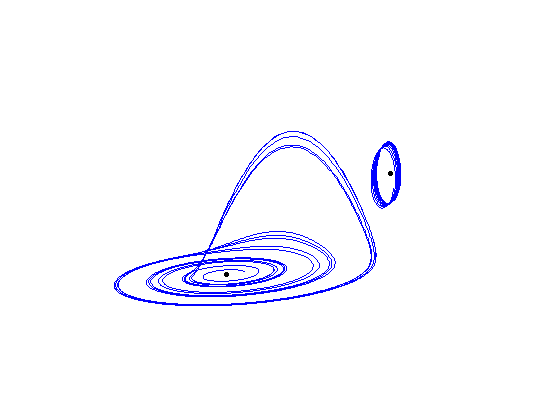
\includegraphics[width=0.35\textwidth]{trajectories}%
%~~~~~~~~
%(b)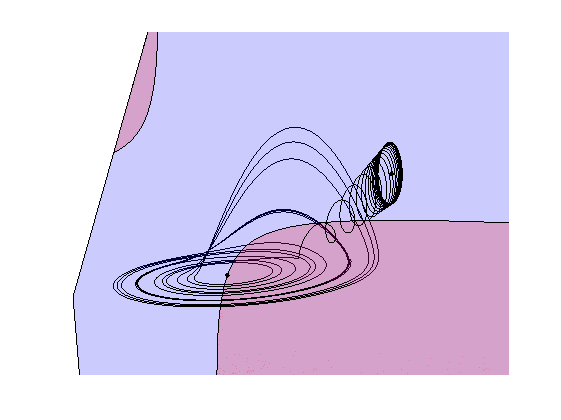
\includegraphics[width=0.35\textwidth]{nearequilibrium}%
 \end{center}
 \caption{\label{fig:neareq}
(a)
Trajectories near the equilibrium for R\"ossler
(see \reffig{fig:RoessTrjs}).
(b)
Near equilibrium Poincar\'e section
(see \reffig{fig:RoessTrjs}\,(b)).
    }
 \end{figure}

 \begin{figure}[H]
 \begin{center}
%(a)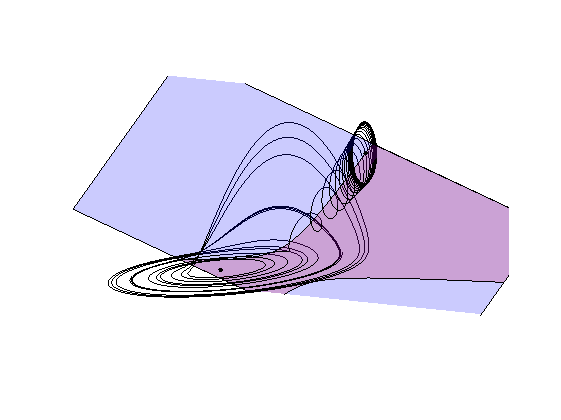
\includegraphics[width=0.35\textwidth]{farequilibriumpoincare}%
~~~~~~~~
%(b)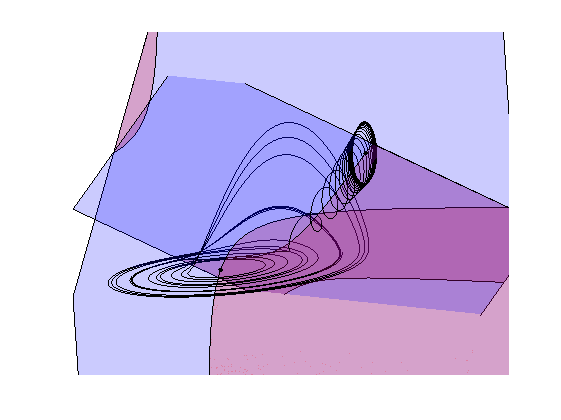
\includegraphics[width=0.35\textwidth]{twoplanepoincare}%
 \end{center}
 \caption{\label{fig:twoplane}
(a)
Far equilibrium Poincar\'e section.
(b)
Both planes superimposed.
    }
 \end{figure}


\item[2012-04-10  Predrag] renamed, moved
\reffig{fig:neareq}\,(a) to \reffig{fig:RoessTrjs};
\reffig{fig:neareq}\,(b) to \reffig{fig:RoessTrjs}\,(b);
\reffig{fig:twoplane}\,(a) to  \reffig{fig:RoessTrjs}; and
\reffig{fig:twoplane}\,(b) to  \reffig{fig:RoessTrjs}.
Please prefix names to all R\"ossler figures by Roess*.png, and \cLe\ figures
by CLE*.png, otherwise they are hard to identify amongst many figures in
siminos/figs/ . From now on, enter comments, update info in
\refsect{s:figures}. Give the improved figure the same name, to save up
on book-keeping (old versions are in the repository, if we ever need
them)

\item[2012-04-10 Bryce to Gang]
Nailed down the method for plotting plane, just need to go do it...
Bright and early tomorrow morning. I also added a positioning statement
to your figures Keith so that they fall below your blog entry.


\item[2012-04-10 Daniel to Keith \& Bryce] The planes themselves look
better than the arrays of points that are in \reffig{fig:RoessSct1}. It's
nice that they are see-through. I would probably make them a little more
so. I'm not sure I'm a huge fan of the color palette, either. I think the
viewing angle isn't great, in the sense that you can't really tell where
the planes are cutting. I think that a viewing angle closer to what Bryce
used in \reffig{fig:RoessSct1}, may work better. I also don't understand
why some of the sections are cropped. I think they would look better as
rectangles. Finally, I would make them both roughly the same size (area).
The little section on top of the huge section looks weird. Another
thought (and I'm not sure how horrible this would be to implement), what
if you drew small points where the trajectories actually hit the
sections? Points don't respond to the alpha command in Matlab, so they
would look like nice dark colored points on the partially transparent
sections of the same color. You could do good crossings in one color and
bad crossings in another.

\item[2012-04-10 Daniel to Predrag]
Working on the \cLe\ figures, but was looking at the version of the paper
that was current when I left Tech while I was riding MARTA. I think that
\refsect{s:slice} can be more neatly organized in the following way:
      \begin{itemize}
      	\item{1. Express the goals of symmetry reductions as an intro}
      	\item{2. Quickly go over the methods that don't work for turbulence}
      	\begin{itemize}
      		\item{i. Transformation to polar coordinates}
      		\item{ii. Hilbert Bases}
      		\item{iii. Method of Connections}
      	\end{itemize}
      	\item{3. Explain what the Method of Slices is}
      	\item{4. Explain what it is not}
      \end{itemize}
and then move on to \refsect{s:chart} and the discussion about global
atlases and such. Just a thought. Committed a restructured version of
\refsect{s:slice}, but feel free to revert it if you had a master plan.
I just cut and paste all the material that was already in there in the
order that I explained above and didn't delete/edit anything.

\item[2012-04-10 Bryce to Daneil] I'm working on my own version of the
plots and should have them up sometime tomorrow. Funny thing is on my way
home I had the same idea of plotting the points where the trajectory
intersects the sections. I think I have figured out a way to implement it
too, we'll see how it looks...

\item[2012-04-11 Predrag to Da Neil] Regarding the outline: Suggestions
sound good to me. As to the order we present them - my ambition is that
we cut to the chase as soon as possible, refer for details to previous
publications and ChaosBook, and postpone all remarks to what this is not
to after we made the reader contemplate the two-chart atlas.

\item[2012-04-10 Daniel]
    Since we are talking about coherent structures in the context
    of turbulence, should we distinguish `exact' coherent structures from
    Lagrangian coherent structures, POD modes, etc?
 \\
{\bf [2012-04-11 Predrag]: } Bit of erudite remark. I would rather be as
brief and to the point as honestly possible.

\item[2012-04-10 Daniel] I cropped the extra white space out of the
figures that Keith posted last night (while keeping them all the same
size), so they don't look so tiny in the text. I have been working on the
figures for \cLf. the The 2-chart atlas one is really busy. Trying to
figure out how to go a little bit more minimalist. In the meantime here
are updates for \reffig{fig:CLf01group}
with full Inkscape axes and labels. What do you guys think? I believe I
have included all the features that we want in \reffig{fig:CLEWurst}, so
I'm going to check it off the to-do list. Let me know if you think of any
other changes that are necessary. As far as \reffig{fig:CLf01group}\,(a)
goes, do we want to try to include \cycle{01}-cycle or $\REQV{}{1}$? Let
me know and I'll update this. \\
{\bf [2012-04-11 Predrag]: } I think it is as good as is.


\begin{figure}
%	\begin{center}
%  	\setlength{\unitlength}{0.25\textwidth}
%  	\begin{picture}(1,1.06440474)%
%    	\put(0,0){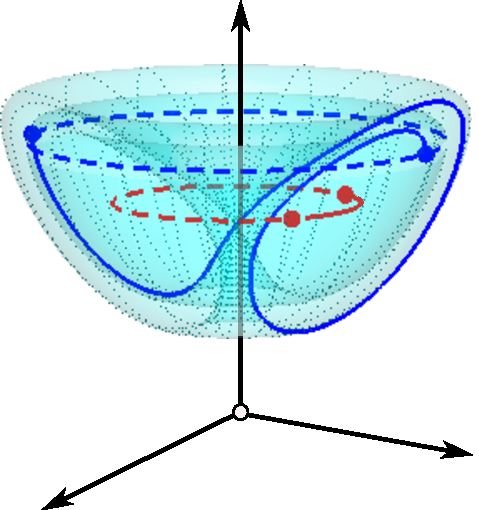
\includegraphics[width=\unitlength]{CLEWurst01}}%
%   		\put(0.55961552,1.00214901){\color[rgb]{0,0,0}\makebox(0,0)[lb]{\smash{$z$}}}%
%   		\put(0.07008555,0.07304272){\color[rgb]{0,0,0}\makebox(0,0)[lb]{\smash{$x_1$}}}%
%    	\put(0.90381504,0.16283301){\color[rgb]{0,0,0}\makebox(0,0)[lb]{\smash{$x_2$}}}%
%  	\end{picture}	
%  \end{center}
  \caption{\label{fig:CLEWurst}
  Replacement figure for \reffig{fig:CLf01group}. One additional feature,
  shown (solid red line) the trajectory of $\REQV{}{1}$ during the 16
  periods of the \rpo is shown in solid red.
  {\bf [2012-04-12 Predrag]} moved to \reffig{fig:CLf01group}.
  }
\end{figure}

\item[2012-04-11 Bryce to Gang] My plots in Mathematica are starting to
look really good! I have TA duties for a few hours and will commit the
final plots later this evening. Obligations, obligations...

\item[2012-04-12 Bryce] After much deliberation I finally have my
rendition of the R\"ossler flow atlas completed. I've added two plots for
the near and far equilibrium as well as their union. Feel free to comment
away. The code is completely set up so modifications from here on out
should be rather painless (lengths of arrows, color schemes, viewing
angles, etc...).

 \begin{figure}[H]
 \begin{center}
% (i)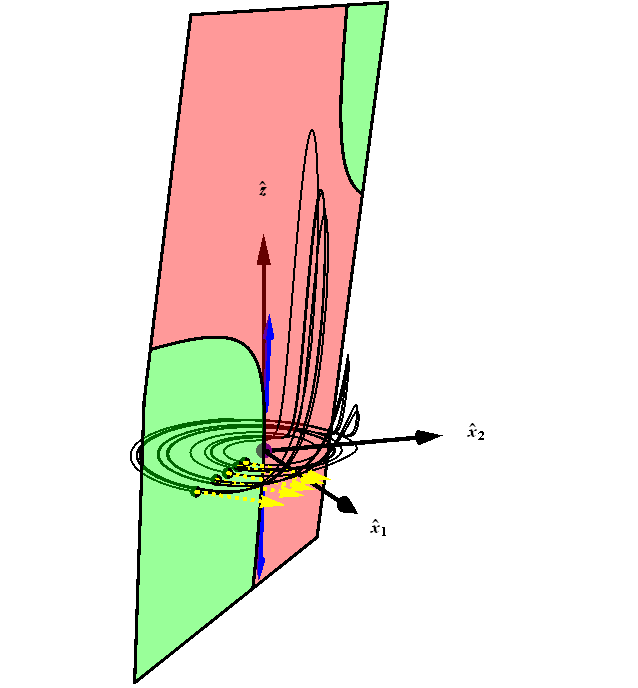
\includegraphics[width=0.45\textwidth]{RoessNearEq2.png}
% (ii)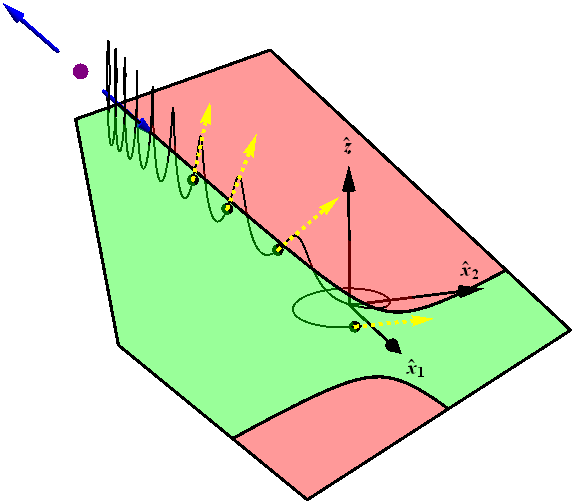
\includegraphics[width=0.45\textwidth]{RoessFarEq2.png}
% (iii)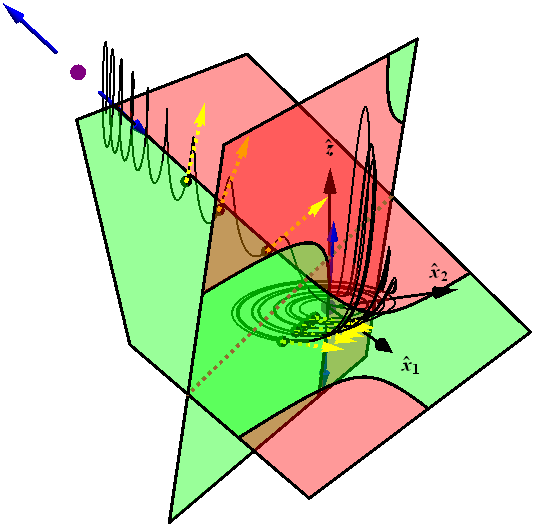
\includegraphics[width=0.45\textwidth]{RoessSctAtlas2.png}
 \end{center}
 \caption{\label{fig:roesslerSections}(i) Section for near equilibrium of
 R\"ossler flow. (ii) Section for far equilibrium of R\"ossler flow.
 (iii) Atlas for R\"ossler flow. \\ \\The points where the trajectory
 intersects the sections are highlighted in black and the velocity at
 these points by a yellow vector. The green and red tones represent the
 points along the section for which $v(\hat{x})\cdot\hat{n}>0$ and
 $v(\hat{x})\cdot\hat{n}<0$ respectively. The purple points indicate the
 equilibrium points while the blue vectors emanating from these
 correspond to the stable/unstable eigenvectors. The brown line line in
 the atlas corresponds to the ridge between the two sections.
 {\bf [2012-04-12 Predrag]} moved to \reffig{fig:RoessTrjs}\,(b). Please update the
 captions there.
 }
 \end{figure}

 \item[2012-04-12 Lei] Also trying to draw some pictures of sections for
 R\"ossler flow, using python. See \reffig{fig:RoessSecPy}
 \begin{figure}[H]
 \begin{center}
 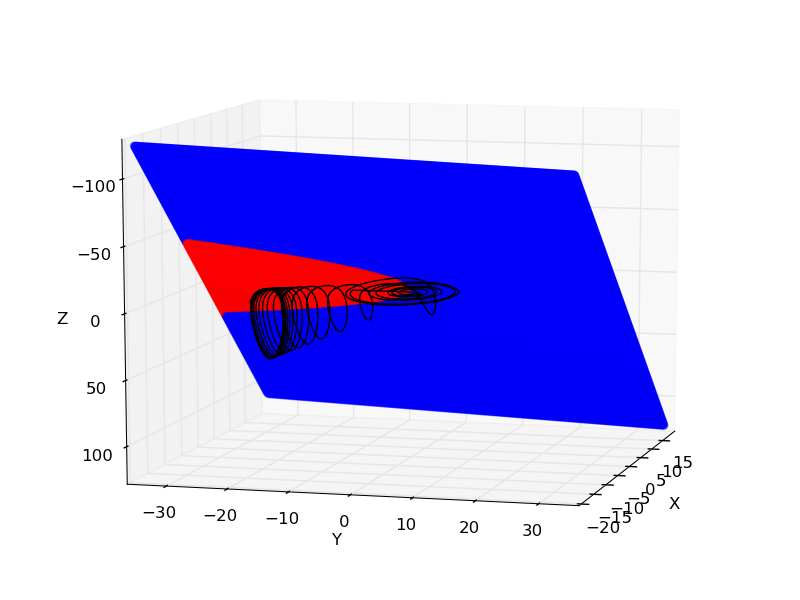
\includegraphics[width=0.8\textwidth]{RoessSecPy.png}
 \end{center}
 \caption{\label{fig:RoessSecPy}}
 \end{figure}

\item[2012-04-12 Bryce] The code I used to produce figure
\reffig{fig:roesslerSections} is now in the course directory on dropbox.

\item[2012-04-12 Predrag] to the C Gang: Lei's is a nice start, but let's
go with Bryce's R\"osslers - we'll edit them, but later, this is good
enough for the submission. Still need \reffig{fig:RoessTrjs}, see
\refsect{s:figures} for desiderata. Somebody still needs to at least read
This Thing, if not (gasp!) write it.

\item[2012-04-12 Daniel]
    Since we are using them as section templates, should the equilibria
    be called $\hat{x}'_{\pm}$ for consistency? Predrag: Thy will be
    done. You can see that having LaTeX macros in figures is not so
    stupid, after all.

\item[2012-04-12 Predrag] to the C Gang: this is not
\HREF{http://www.phdcomics.com/comics.php?f=1485}{how one writes a paper}.

[2012-04-12 Keith to Predrag] It appears I have been doing grad school
all wrong...

\item[2012-04-12 Keith] Added a last paragraph to the slice section.  It
may or may not be liked, but I was hoping to add it as a bridge to the
next section and provide motivation for the previous R\"ossler section;
also it seems like we danced around saying it in the
conclusions/throughout the paper.  This may also provide at least some of
the talking points for the item in the introduction:
      ``section {\PoincS} vs slice \pSRed.''

\item[2012-04-13 Predrag] very  good - I'll merge your text with the
Poincar\'e blah-blah sprinkled elsewhere

\item[2012-04-12 Daniel] Not a huge fan of $t_n$. It could be confused with
    $t_N$. Kinda subtle. Predrag: redefined the macro, so now it is
    $\zeit_n$. Do you like macros now?

\item[2012-04-12 Keith]
I want to call doubt into the caption for \reffig{fig:CLf01group}\,(d).  It
claims the purple are in the wrong direction.  Is that correct?  If so
I'd like to debate this. Or is purple the crossing from 1-chart to the
other, so it should be part of the ridge. Maybe it is just the choice of
words.

\item[2012-04-13 Predrag]
I'm probably wrong. Let's wait for Daniel's girlfriend to let him draw
the \cLe\ figures, and then edit the caption(s).

\item[2012-04-13 Keith] I do not understand the paragraph (posted below),
in the symmetry section.  I do not doubt its accuracy and am willing to
change it, but I do not understand it enough to make a change to it:

The strange attractor of the \cLf\ is shown in
\reffig{fig:CLf01group}\,(a). It's a mess. Why? The problem of dynamics
in presence of symmetry can perhaps be understood this way: dissipative
flows settle into solutions with low friction, and as drifting is
energetically cheap, rather than do work, solutions tend to drift along
non-shape-changing symmetry directions which burn no energy.
A continuous symmetry leads to drifting invariant solutions.
A {\em \reqv} (traveling wave, rotational wave, ...) is a trajectory
whose velocity field lies within the group tangent space,

\item[2012-04-13 Predrag] It's probably a lie. Will ponder...

\item[2012-04-13 Predrag]                   \toCB
Cartography (from Greek $\chi\alpha\rho\tau\eta\varsigma$, chartes =
sheet of papyrus and graphein = to write)

\item[2012-04-13 Daniel] I think I understand what the paragraph that Keith
commented on says and it makes \emph{logical} sense to me, but I wonder how
much of an unsubstantiated claim it is. Anyway, I tried editing it to see if I
could make it clearer. I have claimed red as the color for my edits (ChaosGang
can change their in defAtlas.tex if you want)

On a different note: Shouldn't the two points on $\pS_{\ssp(\zeit)}$ in \reffig{fig:BeThMovFr}
come from different points on  $\pS_{\ssp(0)}$?

\item[2012-04-13 Keith] Worried about something serious, but in the short run, Daniel, for a "bad" template, use a slice only along the $x_1$ or any axis other than $z$.  When I was playing around the reduced state, these never worked.

\item[2012-04-13 Daniel] Here's a stab at the 2-chart atlas for \CLf , see \reffig{fig:CLE2chart2}.

\begin{figure}
  	\begin{center}
  		\setlength{\unitlength}{0.20\textwidth}
  		\begin{picture}(1,0.99328352)%
    		\put(0,0){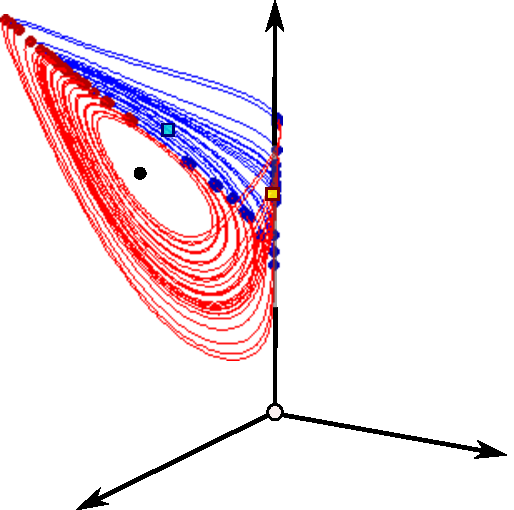
\includegraphics[width=\unitlength]{CLE2Chart.pdf}}%
    		\put(0.58904102,0.9342544){\color[rgb]{0,0,0}\makebox(0,0)[lb]{\smash{$z$}}}%
    		\put(0.13222028,0.06816217){\color[rgb]{0,0,0}\makebox(0,0)[lb]{\smash{$x_1$}}}%
    		\put(0.91024192,0.15195282){\color[rgb]{0,0,0}\makebox(0,0)[lb]{\smash{$x_2$}}}%
  		\end{picture}
    \end{center}
  \caption
  [\CLf: 2-chart Atlas]{Inkscaped version of 2-chart atlas for \CLf. The two templates are shown by the yellow and cyan squares. The crossings between charts are indicated by red and blue dots, so effectively they do sort of mark good and bad crossings of the Poincare section defined by the ridge. You just have to pick which one is the ``right'' direction. That being said, this is not a ``good'' section since it misses some of the spiraling out that a section through the equilibrium would catch. $\REQV{}{1} \rightarrow \EQV{}{1}$ is shown as a black dot.}
\label{fig:CLE2chart2}
\end{figure}

\item[2012-04-13 Daniel] Thanks for the tip, Keith. It sort of does the
trick (although I think this is artificial, since if you take something
with only $x_1$ or $x_2$, but no $y_1$ or $y_2$ components, then the
tangent will always have 0 components in the y's. This means that the dot
product of the group tangent vectors of the template and trajectory goes
to zero more often than if you picked something that has y components.
This adds kinkiness where you wouldn't see it otherwise). Anyway, here's
an inkscaped single slice of the attractor (see
\reffig{fig:CLEAttractorSlice}). At least you can see the kinks
clearly... I think that we should see if we can get the stuff that Lei's
been working on, in such a way that hopefully doesn't have the problem of
large (but non-diverging) phase velocity near some points. We could then
generate something better. Am going to move on to editing for now... Post
comments and suggestions about the figures and I'll try to address them.

\begin{figure}
  	\begin{center}
  		\setlength{\unitlength}{0.20\textwidth}
  		\begin{picture}(1,0.99328352)%
    		\put(0,0){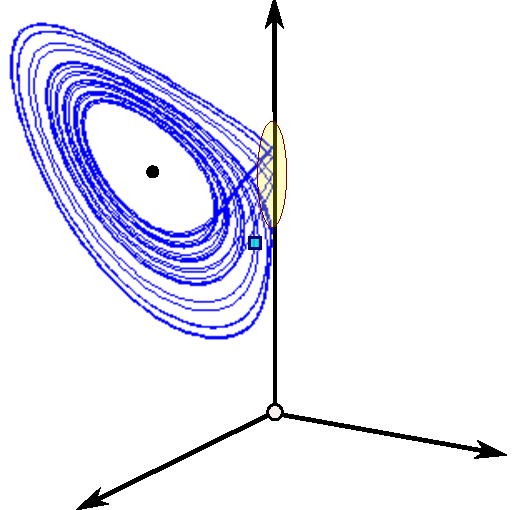
\includegraphics[width=\unitlength]{CLEAttractorSlice.pdf}}%
    		\put(0.58904103,0.9342544){\color[rgb]{0,0,0}\makebox(0,0)[lb]{\smash{$z$}}}%
    		\put(0.13222028,0.06816216){\color[rgb]{0,0,0}\makebox(0,0)[lb]{\smash{$x_1$}}}%
    		\put(0.91024189,0.15195281){\color[rgb]{0,0,0}\makebox(0,0)[lb]{\smash{$x_2$}}}%
  		\end{picture}    \end{center}
  		\caption[\CLf: 2-chart Atlas]{Inkscaped version of single slice for \CLf. The template is shown by the cyan square. $\REQV{}{1} \rightarrow \EQV{}{1}$ is shown as a black dot. Kinks are highlighted by yellow region. I think these are due to the fast rotation near z-axis, not a real divergence of the phase velocity as in \refref{FrCv11}. }
			\label{fig:CLEAttractorSlice}
\end{figure}

\item[2012-04-13 Keith] So I mentioned earlier I was worried about something; I have thought it through and ran the simulations, and it seems that my initial concerns are correct.  To start, when we define a slice, we have to be extremely cautious; for simplicity, lets talk about a slice at $x_1 = 0$.  If we look at the post-processing method, we recognize that we have to define the slice as existing in the $x_2 > 0$ part of space.  Similarly the dynamics run in a slice should have this, otherwise, we have a problem (a group orbit could be put either into the $x_2 > 0$ or the $x_2 <0$ section).  It seems to me then that there is a disconnect between the post-processing method and our "2-chart" atlas.  By this I mean, we either need:
\begin{itemize}
        \item to state that the dynamics are restricted to the entire slice

        \item OR to change the condition for crossing the ridge (\refeq{eq:chartBord})
\end{itemize}
    For example, if I take one of the relative periodic orbits, and run the dynamics in two slices:
    \begin{center}
$\slicep{}^{(1)} = [0, 1, 1, 0, 0]$

$\slicep{}^{(2)} = [1, 0, 0, 1, 0]$
    \end{center}
     \begin{figure}
 \begin{center}
 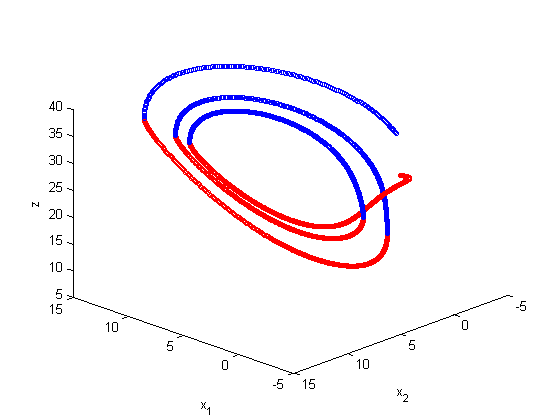
\includegraphics[width=0.4\textwidth]{4atlasmaybe.png}
 \end{center}
 \caption{Dynamics run in two slices with \refeq{eq:chartBord} as the
 condition to cross.  Note the discontinuity that exists because we cross
 the ridge in the wrong part of space.  The two colors (red and blue) are
 the two different slices $\slicep{}^{(1)} = [0, 1, 1, 0, 0]$,
 $\slicep{}^{(2)} = [1, 0, 0, 1, 0]$}{\label{fig:4chart}}
 \end{figure}
 \begin{figure}
 \begin{center}
 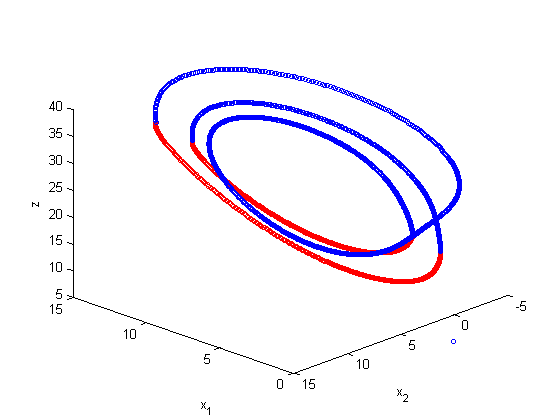
\includegraphics[width=0.4\textwidth]{2atlasforsure.png}
 \end{center}
 \caption{Dynamics run in both slices and then crossed the ridge at the
 appropriate time.  Notice how the discontinuity has disappeared.  The
 two colors (red and blue) are the two different slices $\slicep{}^{(1)}
 = [0, 1, 1, 0, 0]$, $\slicep{}^{(2)} = [1, 0, 0, 1, 0]$
} {\label{fig:true2chart}}
 \end{figure}

After I run these, I then use the condition suggested in
\refeq{eq:chartBord}, there is a discontinuity in the dynamics (see
\reffig{fig:4chart}).  The reason for this discontinuity is because one
can (and as I show) cross the ridge, but not be in the right part of the
slice.  This is why I am suggesting we either fix the slice to cover the
entire space, or we change the condition for crossing the ridge in
\refeq{eq:chartBord} to include being in the correct part of space.  If
we update the condition to have to be in the right side of the space, we
arrive at \reffig{fig:true2chart}.

\item[2012-04-14 Predrag] Keith, I'll try define more clearly what is a
chart and what is a slice later today. Your example is useful in showing
what a bad choice of \template s is, and we will continue with it
starting Monday, as well as the 2-modes model (Lei, please keep working
on it). I believe that Daniel's result of [2012-03-29] is correct, so
that goes into the paper as illustration of 2-chart atlas, even though it
does not illustrate \chartBord s.

\item[2012-04-13 Keith]
The reason we never saw this before is because we started in one slice,
then when we met the condition given by \refeq{eq:chartBord}, we just ran
it in the other slice. The problem is of course that we did not bother to
check which part of the slice we were in.  Therefore, if we define our
slices to only be half the space, then all "2 atlas charts" that Daniel
has been making could in fact be "4 atlas charts".  This explains the
discontinuity in \reffig{fig:4chart}: the ridge condition was met but for
the wrong side of the slice.  This seems to me to be a problem, and while
I am willing to make the changes, I want to know which everyone thinks is
the better solution.

\item[2012-04-14 Predrag] The train is almost gone - I have to submit
tomorrow and what we need in the paper is Daniel's result of [2012-03-29]
above, \reffig{fig:unsliced}, nicely plotted, and the paper finalized
(leading paragraph, etc). There will be time to improve a bit it while it
goes to referees.

\item[2012-04-14 Keith] Ok this seems fair to me; I just was worried
there was something implicitly incorrect.  Sorry for the loss of the day.

\item[2012-04-14 Daniel] I thought I already did a nice version of
\reffig{fig:unsliced}. It is \reffig{fig:CLf01group}. Is that not ok?
Tell me what you want changed and I'll fix it.

\item[2012-04-14 Predrag to Daniel] finalize \reffig{cLe-2chartsDB}.

\item[2012-04-14 Daniel]
I agree with Keith that one has to be careful about the crossings because
otherwise you can get weird stuff happening as I pointed out on
2012-04-06 or as Keith pointed out. Anyway, I agree with Predrag that
that is not something that is going to get resolved by tomorrow. Will
edit some more and get back to you guys. Predrag, is there any part that
still needs to be written up that you would like me to take a stab at?
Let me know.

\item[2012-04-14 Predrag to Daniel] Do important stuff: Finalize the
title, abstract (do we need it? or is it replaced by the lead
paragraph?), lead paragraph (read Chaos J. requirements) and conclusions.

\item[2012-04-14 Predrag to Daniel] Then prepare the submission letter. I
still have to produce the first draft of chart.tex and bridge.tex.

\item[2012-04-14 Keith] Daniel, yes you did point out there may be issues
with the ridge condition, but I fear I may have missed the boat on
understanding that at the time.

\item[2012-04-14 Predrag to Daniel] can you fix \texttt{refref} macro so
it does not look like this:
``see \refref{SiCvi10}?''
but like this: ``see ref.~5?''

\item[2012-04-14 Predrag]       \toCB
\HREF{http://dictionary.reverso.net/english-cobuild/dynamic}
{Dynamics}:

\begin{description}
\item[n-count]  The dynamic of a system or process is the force that
                causes it to change or progress.
\item[n-plural] The dynamics of a situation or group of people are the
                opposing forces within it that cause it to change.
\item[n-uncount]  Dynamics are forces which produce power or movement.    (technical)
\item[n-uncount]  Dynamics is the scientific study of motion, energy, and forces.
\end{description}

I always write ``dynamics is ...'' rather than ``dynamics are ...''. Have I been wrong for 47 years?

\item[2012-04-13 Daniel]
Are we using $\cal{S}$ for both section and slice borders? Predrag: Yes. Economy of Latin alphabet.

\item[2012-04-14  Predrag]
I would love a nice photo or drawing of an onion sliced.

\item[2012-04-14 Predrag]       \toCB
Open question\rf{atlas12}: replace the term `symmetry reduction' by a term that does not
    (1) does not imply `reduction' (2) does not conflict with Lie theory
    and gen. relativity meaning of the term?

\item[2012-04-14 Keith] Here are some of the images we talked about earlier (see \reffig{fig:2poin} and \reffig{fig:bothpoin}).  The only things that don't seem to come up super well are the stable/unstable directions at the equilibriums.  Also the arrows do not seem to come up well in matlab.  Perhaps there is a trick to fixing this.  These are now general enough that I can fix them on demand as needed.  Bryce, did you rotate one of your planes (the far equilibrium one)?
    \begin{figure}
    \begin{center}
    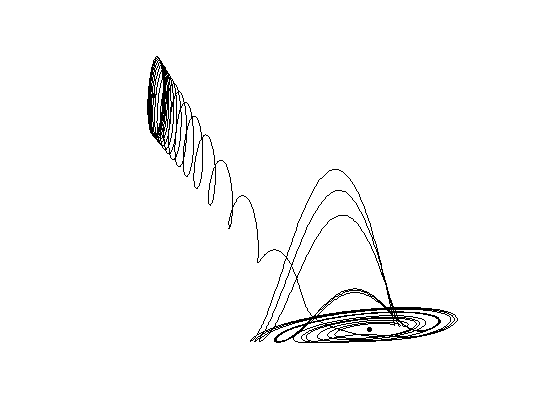
\includegraphics[width=0.35\textwidth]{traj.png}%
~~~~~~~~
    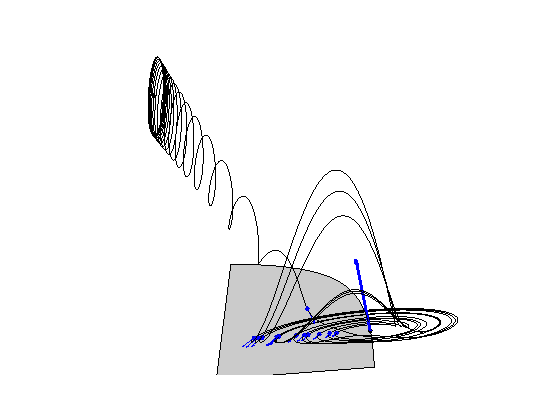
\includegraphics[width=0.35\textwidth]{neareq.png}%
    \end{center}
    \caption{
    (a)
    Trajectory coming from the far equilibrium to near equilibrium
    (b)
    Near equilibrium Poincar\'e section.  The blue dots and arrows show
    where the trajectory crosses and the flow at the crossing.
        }{\label{fig:2poin}}
 \end{figure}

 \begin{figure}[H]
 \begin{center}
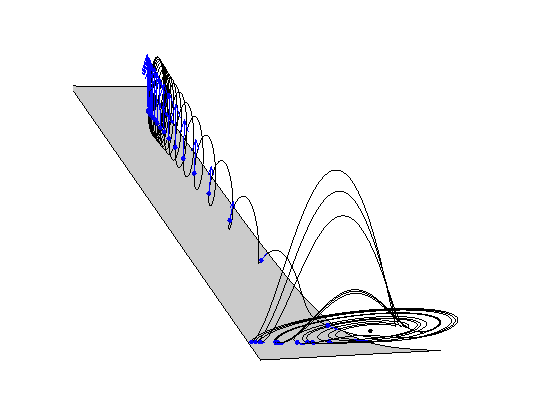
\includegraphics[width=0.35\textwidth]{fareq.png}%
~~~~~~~~
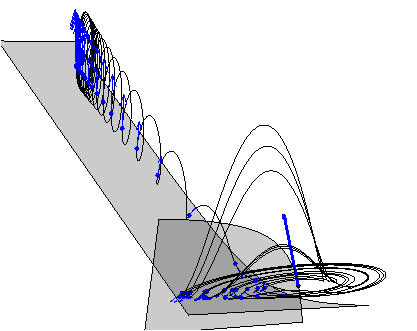
\includegraphics[width=0.35\textwidth]{both.png}%
 \end{center}
 \caption{
(a)
Far equilibrium Poincar\'e section. The blue dots and arrows show where
the trajectory crosses and the flow at the crossing.
(b)
Both sections superimposed.
    }{\label{fig:bothpoin}}
 \end{figure}

\item[2012-04-14 Keith] Just read through log: Bryce, see if you can
replicate the images I posed above; the graphics from Mathematica look
much better and simpler to read.  All you want is the interesting areas,
where the trajectories cross correctly the Poincar\'e sections.

\item[2012-04-15 Predrag to Keith] I like them, except for the girly men
pink - make it gray. I think both.png is wrong: the ridge is above the
strange attractor, the outer section does not reach that far. See
\reffig{fig:RoessTrjs}\,(d). You guys decide which ones illustrates the
2-chart atlas  best, both of these sets are acceptable for me.


\item[2012-04-15 Predrag to Bryce] RoessTrjs2.png is turned 180$^o$ wrong
way - the attractor should be identical in the 4 frames, like in Keith's
girly depictions.

\item[2012-04-15 Keith to Predrag] My wife picked out the color; its her
favorite color.  Reposted the images.

\item[2012-04-15 Predrag to Keith]
Some Victoria Secret hue I would not know anything about.

\item[2012-04-15 Predrag] I like aspects of both R\"ossler sets:

\begin{itemize}
  \item can drop $\{x,y,z\}$ in Bryce's plots, but do keep the eigenvectors
  \item Keep Bryce's planes, hyperbolas, ridge lines in
        \reffig{fig:RoessTrjs}\,(b) and \reffig{fig:RoessTrjs}\,(c).
  \item all 4 frames should have the identical R\"ossler, like Keith's
  \item \reffig{fig:RoessTrjs}\,(d) like Keith's, charts only
  \item Keith's \reffig{fig:bothpoin}\,(b) is now in subdued nordic mood, but still
        wrong.
  \item I like that Keith's are 1/10 of Bryce's (matters for ChaosBook)
  \item now Keith's have huge white margins - crop them tightly, always.
        Did I forget to mention that?
  \item we still have no 2-chart for \cLe, and the day is today
\end{itemize}

\item[2012-04-15 Bryce]

Keith: I will certainly give it a shot. I can reduce the size of the
plane that resides on the attractor so that it doesn't squash everything
else. However, do we still want to keep the domain large enough so that
we clearly distinguish the \poincBord s?

Here are my updates:
  	\begin{itemize}
  	\item Reproduced R\"ossler flow images to include ridges, higher
          resolution, and removed accents on axes labels.
  	\item Added commentary to figures, addressed a few typos throughout paper.
  	\item Started editing the charting section definitions. Still needs quite a bit of work.
  	\end{itemize}

\item[2012-04-15 Predrag to Keith] Now your plots are getting too busy -
hard to see all these arrows, better to remove them.

I think
\texttt{both.png} in \reffig{fig:bothpoin}\,(b) is wrong: The outer
$\slicep{}^{(+)}$ chart ridge with the inner one stops it from descending
down to the attractor. Added explanatory text to \reffig{fig:RoessTrjs}.
Remember, charts intersect orbits only once.

Mark the ridge both in \reffig{fig:2poin}(b) and
\reffig{fig:bothpoin}(a), then clip both at the ridge before putting them
together in \reffig{fig:bothpoin}\,(b)?

 \begin{figure}[H]
 \begin{center}
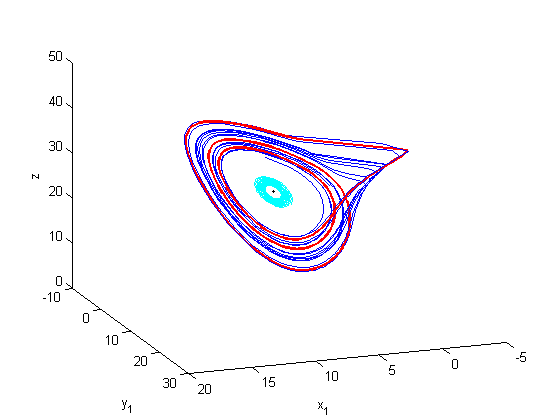
\includegraphics[width=0.35\textwidth]{fullimage.png}%
~~~~~~~~
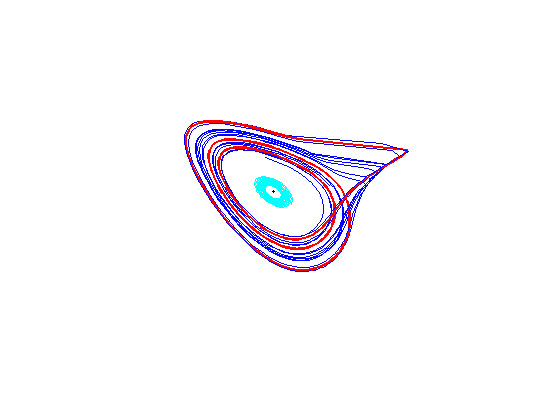
\includegraphics[width=0.35\textwidth]{noaxisimage.png}%
 \end{center}
 \caption{
(a)
Strange attractor of complex Lorenz equations.  Black is both the
template choice and the group orbit $\slicep = \ssp_{\REQV{}{1}}$.  Red
is a relative periodic orbit, I forget which now since I toyed with all
of them.  Cyan and blue are two trajectories.
(b)
Strange attractor of complex Lorenz equations.  Black is both the
template choice and the group orbit $\slicep = \ssp_{\REQV{}{1}}$.  Red
is a relative periodic orbit, I forget which now since I toyed with all
of them.  Cyan and blue are two trajectories.
    }{\label{fig:reducedspace}}
 \end{figure}

\item[2012-04-15 Keith to Predrag]  Ok I'll make those changes; it will
take some time to code the ridge into matlab. Should I just cut of the
sections for as a whole or have the near section look like an "L" since
there is a mismatch between the edges?  Also, is
\reffig{fig:reducedspace} what you are looking for in
\reffig{fig:CLf01group}?  If so, I can crop this, and may be able to put
axis labels in, matlab is a brat about these things. Also this had to be
done by postprocessing.  If I tried to do the dynamics in the slice, the
minute it hit near the discontinuity it would diverge quickly.

\item[2012-04-15 Predrag to Keith] R\"ossler: it is true that the
\PoincBord\ is not continuous over the ridge, but that is OK, as long as
the trajectories of interest are way from the borders.

\item[2012-04-15 Predrag to Keith] It's too late for a new \cLe\
attractor image. I have asked Evangelos to join is - we will use his
\texttt{CLEperpReqb} in \reffig{fig:CLf01group}\,(c), and he will help
Lei with the 2-mode model simulations in the coming weeks.


\item[2012-04-15 Predrag to Keith] The whole point of two charts well
placed is that you do not ``hit near the discontinuity it would diverge
quickly.'' But it's too late for that. Why don't you proofread, edit the
article until and including sect IV, and the conclusions. I'm working on
V and VI.

\item[2012-04-15 Predrag] If no miracle happens in the next couple of
hours, I'll have to cheat, and use \reffig{fig:CLf01group}\,(d) and
Inkscape to fashion something like a 2-chart atlas.

\item[2012-04-15 Bryce] Making my way through the sections all the while
editing, cutting, trimming it down. Working on the rough transitions
between paragraphs.

\item[2012-04-15 Keith] is the line:
Given distances and neighborhoods,
the next key notion is  \emph{measure}, or how likely a typical
trajectory is to visit a given neighborhood.

necessary? it doesn't seem to fit since we don't really talk about measures.

\item[2012-04-15 Bryce to Keith] We don't spend a great deal on the study
of measures but the notion of picking a smart template to represent a
neighborhood is discussed in some detail. A slight rewording of the
sentence or the one following might make it clearer...

\item[2012-04-15 Predrag to Keith] the very notion of template is the
notion of `measure' - we pick templates from regions where requrances are
frequent, \ie, the measure is large.

\item[2012-04-15 Keith]  Notation question, for the definition of chart,
should it not be $\pS/\Group \supset$ \emph{chart} $\pSRed{}^{(1)}$
instead of \emph{chart} $\pSRed{}^{(1)} \supset \pS/\Group$.  Since a
chart may not fully cover the {\reducedsp}?

\item[2012-04-15 Predrag to Keith] You are right, now I found the error twice
in the manuscript. Not sure how it happened, thanks. The \slice\ never
captures the totality of group orders, only an open neighborhood
(definitions section of the paper).

\item[2012-04-15 Keith] I now understand how the purple in
\reffig{fig:CLf01group}\,(d) is the wrong direction.  This seems slightly
confusing because we are talking about how Poincar\'e sections are not
slices, but then we say the Poincar\'e section points on the ridge.  I
now understand what you mean, but there is big jump at least for me.  We
may want to avoid this issue altogether saying the colors are ridge
crossing or just say "the color green and purple are the ridge crossing.
This ridge could be used as a Poincar\'e section with one direction being
the "good" chart of the Poincar\'e and the other the "bad" region".

\item[2012-04-15 Bryce to Keith] I think that so long as we make the distinction that the points that lie along along the ridge can be viewed, in the spirit of Poincar\'{e} sections, as symmetry reduced trajectories that cut through a d-2 dimensional hypersurface (note sure if it is always a ``plane'' ).

* Also, just a quick sidenote, if you want to put something in quotation marks you need to use `` ` '' and `` ' '' rather than the usual key for quotation marks. Just a LaTeX thing...

\item[2012-04-15 Bryce to Predrag] In \refsect{s:chart} just below the last definition you state ``Here we have defined a slice... as a contiguous set of hyperplane charts...'' I believe the it should read ``Here we have defined an atlas... as a contiguous set of hyperplane charts...''. Revert it back if my assumption is incorrect.

\item[2012-04-15 Bryce] I've now read through the paper in its entirety, fixed things here and there, and added my own two-cents when appropriate. Are we still ``faking'' the CLE 2-chart? I really wish I could get my code to work properly for CLE but I spent hours trying to avoid the discontinuity with the various templates Daniel cooked up but the break conditions I was using in Mathematica's integration routine ended up bouncing me back and forth between templates. I haven't been able to crack my code since then...

\item[2012-04-15 Keith] Read through Bridges to Nowhere.  Not as familiar with the stuff, but I will sift through for grammar.  Only questions, is that white space intentional in between the paragraphs?

\item[2012-04-16 Predrag] Submitted the paper to Chaos Journal -
submission was hell - from 8 pm to 2 am - had to submit and label every
figure by hand, fill in everybody's phone number etc etc - was in bed by
3am. What a way to spend a weekend.

Do not change anything in directory \texttt{siminos/atlas/Chaos-v1} from
now on.

\item[2012-04-16 Predrag to C Gang]
You understand how unprofessional it is to write a professional
publication on the night of the deadline. The final draft of the paper
has to be ready several weeks ahead, to have time to read it critically
and fix problems such as figures that do not print. I still believe the
paper would have been easier to understand if you wrote it, but too late
for that now. I would have let you hang in the wind, were it not that I
had personally asked for and promised to deliver that this paper will be
delivered.

Instructor writing your article does not count as the term project in the
course, so you still have to write your own project - I have created
directory siminos/cgang/ for you, take it from there. I think creating a
\HREF{http://chaosbook.org/tutorials/index.html}{tutorial} with 3D rotatable
simulations would be fun, but maybe that's too ambitious. Up to you.


\item[2012-04-16 Predrag to C Gang]
Will wait for Chaos Gang to finalize the figures, make them small before
submitting the article to arXiv.org - keep proofreading atlas/atlas.tex.

\item[2012-04-16 Ashley Willis] Well done, the article does a good job in
showing the similarities and differences between the method of slices and
the Poincar\'e section.

\refFig{fig:CLf01group}\,(d) didn't print out properly for me, I got a
solid blue block.  In \reffig{fig:CLf01group}\,(b) the jumps are not
obvious.

In \reffig{fig:A29-2slices}\,({\it c}), why have the templates been
placed on the ridge, the templates lie within each other's chart.

Do we not want a more general picture at this stage?  Perhaps
intentionally, the figure does not give a sense that the appropriate chart for
the reduced trajectory to occupy is that of the nearer template.

\item[2012-04-16 Predrag to Daniel] Please respond to
ashleypwillis@gmail.com. I think he is right that we failed to explain
it. In particular, after C Gang has met and discussed the matter, explain
to him that the \template s do not figure in the \slice\ condition
\refeq{PCsectQ0}. Maybe we will have to redraw \reffig{fig:A29-2slices}
accordingly (with $\sliceTan{}{}^{(j)}$ on the ridge, but not the
\template s\ $\slicep{}^{(j)}$?).

\item[2012-04-16 Ashley Willis] I should have looked closer at
\reffig{fig:A29-2tmplts}, not referenced in the text.

\item[2012-04-16 Daniel]
Can't sleep so I resized the CLE figures... The PDF's are now smaller in
physical size (and pretty close to what they would be in print), but
aren't really much smaller in hard drive space. For this I made some
jpeg's, but they don't look nearly as good. PNG's would probably look
nicer but are apparently Chaos does not like to play with them. I also
left the .tex files for the labels in case these change upon rescaling.
Pick and choose what you want to keep or make a new request. Figures are
saved in new directory /atlas/CLESmallFigs, so as not to mess with
anything in the submission documents. Feel free to delete any of the
files in this folder.

\item[2012-04-16 Predrag to Daniel] Nice figures, but PDF's are still way
way too large for eventual inclusion in ChaosBook as *.eps. I think the
way to go is, once we have finalized 2-charts, to convert only the
strange attractor into *.png, then build Inkscape around it. But that is
the very last final step before finalizing the manuscript.

Remember to mention in figure captions that \cycle{01} is drawn. It looks
very wrong in CLEunslicedsmall.* (`small' = 1/2 MB?).


\item[2012-04-16 Keith]
I am interested in trying something; I do not know if it will work out,
but I want to try it anyway to learn for my own good:

So early on, I worked on making the return map for the R\"ossler system,
though it had some rough patches, I still managed to get out periodic
orbits or as close to periodic as possible.  That was a fairly fun task
for me.  So for the project, I'd like to work on correcting that, and I'd
like to try to extend this to the \cLf\ to find \rpo s and the
likes.  Then if I can manage this, I want to try to do the same analysis
in symmetry reduced space.  I have my suspicions about what will happen,
but I do not know for sure.  I admit, part of this is just pure curiosity
as to what will happen, so I wanted to check that this would be OK for
the project.

\item[2012-04-17 Predrag to Keith] Sounds good, but once R\"ossler works,
find \rpo s for the 2-mode problem. We have none, and Lei and Evangelos
need them - they will provide parameters for you (provided they find an
interesting chaotic case).

\item[2012-04-17 Predrag to Chaos Gang]
Start writing up whatever you are doing in the C Gang term project report
in \texttt{siminos/cgang/}. The gang is allowed to reuse any equations
and or figures from the paper I wrote\rf{atlas12} but not a single
sentence penned by me or there will be copyright violation suits. Cannot
steal from Wikipedia either (if you find any website where we
collectively can learn something about slicing, alert me instantly).

\begin{quote}
{\color{red} \large
May 1 2012,  11:30am - 2:20pm term projects due, Predrag's office
}
\end{quote}


\item[2012-04-17 Predrag to Lei] Evangelos (who did the CLE modeling that
we used in the paper) is interested in whether the 2-mode model exhibits
more interesting 2-chart slice than the CLE, so he plans to join you in
searching for interesting chaotic behavior. Do not feel guilty for not
contributing to the paper - we divided the labor between completing the
R\"ossler, CLE and working on 2-mode in parallel, so you were doing your
share.

Critically reading and proofreading the paper - there is still time, as
we have to improve some of the figures before uploading the paper to
arXiv.org.

\item[2012-04-17 Predrag to Daniel] Ashley gets siminos/atlas/ repository
log messages, so if you want to engage the whole C Gang in the
discussion, blog it, address the log message to Ashley.

\item[2012-04-17 Daniel to Chaos Gang] In case you were wondering what
Ashley and Predrag are talking about below, here's what motivated it. In
response to Ashley's comments on the paper from 2012-04-16, I wrote the
following by email:

\begin{quotation}
A point that wasn't clear in the paper is that there is
a lot of freedom for picking templates in the low-dimensional toy systems
(which may or may not transfer over to turbulence, not 100\% sure). For
example, all one ever really check is dot products of things with the
tangent vector t, not with the template x'. So any two templates with the
same t, give the same slice, which is seems sort of weird, so I don't
know that we aren't missing something here. Furthermore, one only checks
when certain dot products are zero, so really one can take x' and divide
it by any constant, and it'll still work exactly the same.
\end{quotation}

\item[2012-04-17 Ashley]
For more than a few degrees of freedom it seems unlikely that two states
would have so similar $\sliceTan{}$.

\item[2012-04-17 Predrag]
The paper\rf{atlas12} emphasizes that as the slice and border conditions
are linear, they depend only on the ray that \template\ \slicep\ belongs
to, not the position of \slicep\ itself. If you are saying that it is
unlikely that the \template\ \slicep\ multiplied by a constant pierces
the strange attractor several times, I agree, but what's the problem if it
does? The paper\rf{atlas12} emphasizes that no information is lost by
symmetry reduction; the two \template s\ on the same ray,
$\slicep{}^{(1)} = A \slicep{}^{(2)}  $, $A=$~const., have distinct group
orbits and are distinct point in the \slice, so what's the problem?

\item[2012-04-17 Ashley]
What concerns me more is that
dotting against $\sliceTan{}$ retrieves no information from $\sspRed$,
the shift-invariant part of $\ssp$.  For pipe flow, this means no
information from the mean flow!, which carries most of the energy.

\item[2012-04-17 Predrag] Don't understand this - are you saying the
$\sliceTan{}$ retrieves no information from $\sspRed$ or the \template\
\slicep? Either way, there is no problem - the reconstruction equation
tells you what the energy in the pipe frame is: The paper\rf{atlas12}
emphasizes that no information is lost by symmetry reduction

\item[2012-04-17 Daniel in complement to Predrag] I think in the full
formulation (where you rewrite the dynamics), this information would be
kept in the integral of the reconstruction equation. Used as a
post-processing method, I guess one would have to keep a record of what
shifts you used to bring your trajectory back to the slice and the mean
flow info would be contained therein.

\item[2012-04-17 Ashley]
If we are only looking for structural similarity, then I guess this is
ok.  But what if structurally similar solutions of different amplitude
have very different behaviours?

\item[2012-04-17 Predrag] For Euler with $\infty$ boundary conditions,
there might be invariant solutions related by particular constants,
$\slicep{}^{(1)} = A_n \slicep{}^{(2)}  $, $A_n=$~const. I've heard of
Putkaradze dream of such things, but as I find renormalization ideas
(other than close to phase transitions or onset of chaos) bad physics and
waste no time on them. I cannot think of any scenario for which this
would happen for \NSe\ in pipe. If there are `structurally similar
solutions of different amplitude' (how could they fit into the same
pipe?) they are distinct \statesp\ points both in the full and reduced
\statesp, they will have very different behaviours, and that would be
just OK. It would be a major miracle if there were two time dependent
solutions of fluid dynamics that differed by a scale factor and
maintained the same dynamics. For infinite pipe that would be only
possible in the streamwise direction. Why are we worrying about this?
Wouldn't it be easier to talk about it instead of writing about it?

\item[2012-04-17 Daniel in complement to Predrag] Mmmmm... I guess the
dynamics are really calculated in the full space without any rescaling,
so maybe that takes care of that? Like when one is trying to figure out
what amplitude perturbation you need to trip pipe flow into turbulence
and you just take a prescribed perturbation and then just tweak the
amplitude. Each one of those perturbations corresponds to a different
point in state space and will be on a different group orbit. I guess they
will just happen to be group orbits that have tangent vectors that point
in the same direction. I guess the nice thing will be that you would be
able to see all of them in the same slice.

\item[2012-04-17 Daniel] One further point that Ashley made was that some
of the lines in the paper may be directly out of \refref{ACHKW11}. I
realize that some the stuff probably got pasted into the paper as notes
on what to include, but we should be careful to either cite these (even
though Predrag is an author on \refref{ACHKW11}) or at least reword them,
so it's not just a straight up cut and paste. I will try to read through
both papers and see if I catch anything but somebody else should too.
\refref{ACHKW11} is available on the arXiv.

\item[2012-04-17 Predrag] I assume I own the text I wrote myself - if you
find something, let me know, I know what I wrote in \refref{ACHKW11}.

\item[2012-04-17 Daniel] It would be nice, though, if sentences weren't copied
verbatim out of another paper. I'll keep an eye open, but perhaps it may be a
good idea for ChaosGang to read through our paper, and then split up the pages
in \refref{ACHKW11} amongst us and try to find and direct cut and pastes. Anyway...
Here are some comments on the \PoincSec part of our paper that I think should be addressed:
	\begin{itemize}
		\item[1.]We claim that, ``The remaining freedom to rotate each section can be
		used to orient them in such a way that the ridge (the intersection of the
		two sections) lies approximately between the two templates (\reffig{fig:RoessTrjs}\,(d)).
		Such a choice guarantees that both neighborhoods will be well represented.'' Is this
		something that we came up with because we couldn't come up with anything else
		(As Predrag and I discussed today, we don't know of a variational principle
		that fixes the two as in the case of slices) or is there something to it. If I
		was reading the paper as an outsider, I think I would find this condition and
		it's matter-of-fact discussion a little speculative and/or confusing. We might
		consider explaining why this is a good choice, even if not a perfect one.
        \\{\bf [2012-04-17 Predrag]} I have no good suggestion on improving these sections
        beyond what we have done.

		\item[2.] The little comment in Greek is nice inside joke, but
        I'm not sure it's necessary. I'm not totally opposed to lame humor but
        it's not necessary.
        \\{\bf [2012-04-17 Predrag]} OK, OK sending
        $\chi\alpha\rho\tau\eta\varsigma$ back to Evangelos. The
        befuddled Chinese who never had classical Greek in high school
        will now be less befuddled.

		\item[3.] In the discussion of \reffig{fig:RoessTrjs}, I'm not
        sure it's clear why 		the section hyperplanes beyond the
        ridge are not part of the atlas. Perhaps we 		should
        include a discussion of jumping between sections? Will think
        about how 		to write this.
        \\{\bf [2012-04-17 Predrag]} E tu Brutus? You, the slayer of \cLe?
        That's the \emph{whole point}, motivating the 2-chart slice atlas
        of 2-chart atlas of \reffig{fig:CLf01group}\,(d). You want the
        trajectory to be cut only once (before next return to the
        section), not twice like Keith insists on doing in
        \reffig{fig:twoplane}\,(b). It's not ``Both planes
        superimposed,'' but the two charts \emph{joined } at the ridge.

		\item[4.] I agree with Predrag that the R\"ossler figures probably still need some work.
		Will try to play around with Keith and Bryce's code.
	\end{itemize}

\item[2012-04-17 Keith]  Back early and had a chance to finally read
through a bunch of the references rather than sift through them.  I do
want to address that \refref{FrCv11}, you cite the slice condition as
being
\[
\frac{\partial}{\partial \gSpace} \Norm{\ssp - \LieEl(\gSpace)\,\slicep}^2
   =
2\, \braket{\sspRed - \slicep}{\sliceTan{}}
   = 0
        \,,\quad
\sliceTan{} = \Lg \slicep
\,,
\]
Which agrees with this paper, but also with the condition that it is a
minimum; you go onto explain that it the condition is a positive
curvature for:
\[
\frac{\partial^2}{\partial \gSpace^2} \Norm{\ssp - \LieEl(\gSpace)\,\slicep}^2
   =
-2\, \braket{\sspRed}{T^2 \slicep}
\]
This was my point on Friday last week: you need to check you are on the
right side of the slice.  I believe this was the point made recently,
your condition for crossing the border states only that you have the
checked the dot product with the \sliceTan{} but you never check if the
above still holds.  In other words, the slice condition is the exact same
if you are at:

$\slicep{}^{(1)} = [x_{1}, x_{2}, y_{1}, y_{2}, z]$
and
$\slicep{}^{(2)} = [-x_{1}, -x_{2}, -y_{1}, -y_{2}, z]$

The condition to check if you crossed to the right side is the same as
the curvature condition.  Was this checked for \reffig{fig:CLf01group}\,(c)?
This could explain the weird jumping thing you were seeing Daniel,
because the only thing that would change if you are on the wrong side of
the slice is the sign of the phase factor (ie it would push you back to
the other chart rather than continuing).

\item[2012-04-19 Predrag]                       \toCB
The discrete charm of a \emph{chart} is that it is defined by minimal
distance, so no need to check the curvatures - that you would do only if
you were looking at the set of solutions to the slice condition. Here you
are guaranteed to have the right one. The moment you cross the
\chartBord\ the curvature changes, but as it is {\color{red} verbotten}
the cross that border, there is never any ambiguity. Charts are
brilliant, nein?

\item[2012-04-19 Daniel]
    Obviously other people have looked at the method of slices... we cite
    them!
\\{\bf Predrag:} I wish you were right, because then we would not have
    to write yet another paper on slices. This is not a paper about
    single slice hyperplane, it is about how you construct an atlas over
    a slice of interest. \refRefs{rowley_reconstruction_2000,BeTh04} only
    study \reqva\ of PDEs, and for that a single slice hyperplane
    suffices, they do not mention anything about \chartBord s - if you
    find them anyplace in literature, please alert me. Ditto for
    \poincBord s, I have never seen them defined anywhere.
    \refRef{SiCvi10} is about \cLe, and notices that there is a
    \chartBord\ (calls it `singularity set') but waffles about it, as it
    has no notion of distance and a chart. \refRef{FrCv11} uses the
    notion of the closest distance first noted in
    \refref{rowley_reconstruction_2000} to define a neighborhood and
    explain the jump induced by \chartBord\ crossing. We tried and failed
    to construct a two-chart for \cLe. \refRef{ACHKW11} is the first and
    still only attempt at implementation of the atlas idea - I fear
    Ashley is in error as long as \reffig{fig:A29-2tmplts}\,(b) is not
    implemented, that is why we never found any \rpo s beyond the lower
    edge of turbulence. But I do not think adding all this info to the
    paper aids the reader one iotta, it only makes the paper longer. I
    can stick all this into remarks in ChaosBook.org, but it's beyond
    point here.

\item[2012-04-19 Daniel]
    Who actually showed \refeq{reconstrEq} first... fix reference
    accordingly.
\\{\bf Predrag:} it's tedious, the history is in the remarks in
    ChaosBook.org continuous.tex, as we say in the introduction - not
    worth getting into this here. Erudition gets into the way here, we
    just want to get to the point as fast and compactly as possible.

    BTW: if you do not use footnotes but embed the editorials
    into the text proper, they do not get turned off when we turn the
    draft switch off - dangerous practice, as if you again make me submit
    the paper at 2AM some of these private doubts will go straight to the
    readers and referees - so I am now again stuck in Howey 9:15PM - no,
    already 10:30PM - with the Memphis blues again, making them into
    footnotes while I would much rather bicycle home and ...zzz...


\item[2012-04-19 Daniel] ``graveyard of obvious ideas'' rings a little
    aggressive, no? ``if you are a master of quantum-mechanics or QFT symmetries
and their linear irreducible representations,\rf{PCgr} you may leave your
baggage at the door'' rings a little aggressive, too.
\\{\bf Predrag:} That's the risk of letting me in the lurch, writing the C
    Gang paper. Get's edgy. In ``master of their linear irreducible
    representations'' I make fun of myself. Let the referee object to
    that? Will not kill the article just because of that, I hope - it is
    a talk written up, so being a bit more colloquial is hopefully OK...

\item[2012-04-19 Daniel] Consider moving this whole part on ridges and such to
    \refsect{s:chart}?
    \\{\bf Predrag} It was there originally, but I moved it because
    in \refsect{s:symm} we define a single chart, and in
    the next section bind them together into an atlas...


\item[2012-04-18 Daniel in response to Keith] Yeah... I'm pretty sure
that is what was happening and it was aggravated by the fact that I
didn't carefully track the crossing. That's why the two slices get mixed
in \reffig{fig:2chartfail}. The fix for \reffig{fig:CLf01group}\,(b) was to
check which way the sign was changing as the dot product went through
zero. Then one only takes zero crossings that go from positive to
negative but not from negative to positive (or vice-versa, I would have
to check). This guarantees that you switch correctly (at least in the
\cLe\ case. That worked in practice, but probably has a more formal
mathematical statement in terms of a variational principle, similar to
what you mentioned above. I think your color coding scheme in
\reffig{fig:4chart}, might be different from what I used in
\reffig{fig:2chartfail} in the sense that you may be on the slice
hyperplanes for the two templates but be coloring them based on what side
of the ridge you are on, rather than what slice hyperplane you are on. I
would need to check to see what my code returns if I use the templates
that you used above but don't check the directional condition. What did
you use as your initial condition? Is that $\overline{011}$?
$\overline{001}$?

\item[2012-04-18 Keith to Daniel] $\overline{001}$.  The slices are the
given above if you want to compare to what I had.  When you say crossings
that go from positive to negative and not from negative to positive, what
do you mean?  The crossing condition you programmed only checks a
crossing or does it check the directionality of crossing?  or was that in
reference the minimum condition? I am curious to see the result and I can
run it if you want, but which is the code?

\item[2012-04-18 Daniel to Keith] My code isn't really ready for general
consumption. I'll clean it up, comment it, and post it for the masses
later. Anyway, the crossing condition is basically checking when the dot
product of the target template tangent and x crosses zero (which is
equivalent to checking the extremal condition (first derivative = 0), but
not the full minimum condition (first derivative = 0, second derivative >
0). When you cross the ridge one way, $\braket{\sspRed -
\slicep}{\sliceTan{}}$ goes from positive to negative, when you go the
other way it goes from negative to positive. I just make sure that I only
count crossings going one way.

\item[2012-04-19 Predrag] You really want \reffig{fig:slice} to be
Victoria Secret (or Secret Service) pink? Whatever...

\item[2012-04-20 Keith] As irony has it, Pink is Victoria Secrets other
merchandize line... The whole thing is a conspiracy. Non sequitur: see
\reffig{fig:RossRedone} and \reffig{fig:RossRedone2} for the updates we
talked about today.  Since I will be out of town for the next few days
for a funeral, I have also taken the liberty of posting the .fig files if
you do not like the perspective, then someone can open them, and rotate
them to what they feel is a better perspective.  I would post the code,
and if you really want it, feel free to ask, but it is very tough to
follow (I have the nasty habit of not commenting a thing).  I posted
these in folders in figSrc/, (they are called Rossler Arrows and Rossler
No Arrows), there is the option of having all the arrows taken away.  If
you want the color scheme changed for some reason or another, let me
know, and I will repost the .fig (since I have to use remote access over
the weekend, I can't actually save the plots I make as .png for an
unknown reason as of now; if anyone knows why if there is a way around
this (its only in remote desktop), let me know, and I will gladly try
it).

Also \reffig{fig:othertraj} is the best I could come up with for showing
circling around the far equilibrium.  It seems like the paper G. F Amalar
et al may have fabricated the image (not necessarily unjustly to show the
rotations).

 \begin{figure}%[H]
 \begin{center}
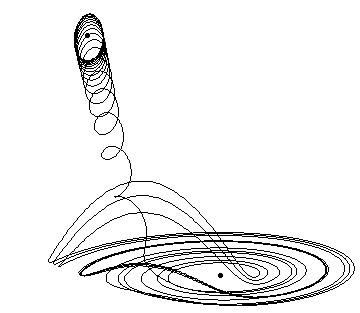
\includegraphics[width=0.35\textwidth]{rosstrajkc.png}%
~~~~~~~~
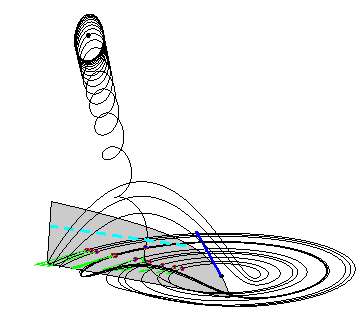
\includegraphics[width=0.35\textwidth]{rossnearkc.png}%
 \end{center}
 \caption{
(a)
R\"ossler trajectory.
(b)
R\"ossler near equilibrium Poincar\'e section (grey).  The crossings of
the section are labeled (red) with velocity vectors at the crossings
(green).  Both equilibrium are shown and for the near equilibrium, shown
is the stable manifold (blue). The intersection with the Poincar\'e
section from \reffig{fig:RossRedone2} is shown as a dotted line (cyan).
    }{\label{fig:RossRedone}}
 \end{figure}

 \begin{figure}%[H]
 \begin{center}
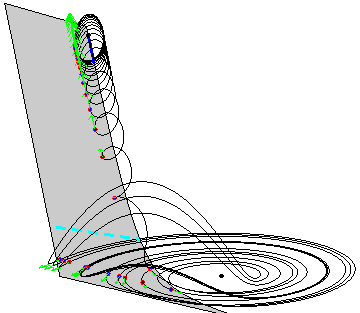
\includegraphics[width=0.35\textwidth]{rossfarkc.png}%
~~~~~~~~
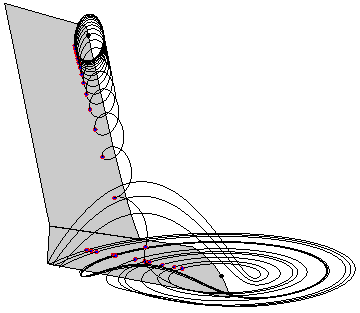
\includegraphics[width=0.35\textwidth]{rossbothkc.png}%
 \end{center}
 \caption{
(a)
R\"ossler far equilibrium Poincar\'e section (grey).  The crossings of
the section are labeled (red) with velocity vectors at the crossings
(green).  Both equilibrium are shown and for the far equilibrium, shown
is the unstable manifold (blue).  The intersection with the Poincar\'e
section from \reffig{fig:RossRedone} is shown as a dotted line (cyan).
(b)
Two Poincar\'e charts depicting the dynamics of the system.  The velocity
vectors and stable/unstable manifolds have been removed, but still shown
are the crossings of the the 2 charts (red).
    }{\label{fig:RossRedone2}}
 \end{figure}


 \begin{figure}%[H]
 \begin{center}
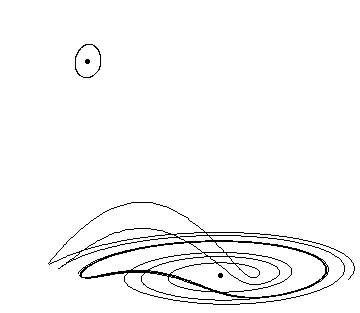
\includegraphics[width=0.35\textwidth]{othertrajectory.png}%

 \end{center}
 \caption{
Attempted remake of the other trajectory.  The image must have been made
up in that paper, because I ran the trajectories forwards backwards, and
everything, and could not reproduce anything that looked like it.
}{\label{fig:othertraj}}
 \end{figure}

\item[2012-04-20 Predrag to Bryce and Daniel] Looks good to me - maybe
you want to play with *.fig's a bit, but when you give a go-ahead we (or
I) can Inkscape a few finnishing touches and prepare the manuscript for
arXiv submission.

\item[2012-04-20 Keith] I also have R\"ossler return maps for a
Poincar\'e section of our choice.  Even though the interesting dynamics
is/are contained in the near equilibrium chart, if you want this, I can
supply, I believe I fixed errors.

\item[2012-04-20 Predrag to Keith] Can you include it in your project report?
Paper is too long and return maps are already in ChaosBook.org and Basu project.
What would be great is to get forward Poincar\'e maps for 2-mode model.

I would put a priority on the Dangelmayr 2-mode model, as \cLe\ seems too
simple. Lei is MIA (last blog entry on 2-mode was [2012-04-10]), you can
perturb his \reqva\ and see what happens in Cartesian coordinates), so
maybe you can just play with it yourself - it's no harder than \cLe,
maybe even easier, it is in 4 dimensions. If there are two distinct
\reqva\ and chaos that hops between them, I hope there is a robust
\chartBord\ separating them, with 2-chart atlas ridging it. That would be
much more persuasive. Besides, the Dangelmayr 2-mode model is known by
many more people than \cLe, would have more of an audience.

It's not guaranteed to work, I'm worried about the role that the
invariant subspace plays - might still turn out not to be too
interesting, even though is should have more \reqva\ than \cLe.


\item[2012-04-20 Predrag to Lei] Can you (and Evangelos?) write up 2-mode
your project in siminos/cgang/Lei/ , blog the progress here so gang is
up-to-date?

\item[2012-04-20 Keith to Predrag]  Yes I was also going to take a look
at the 2-mode this weekend.  I'll see what I can make out.

\item[2012-04-21 Bryce to Predrag] I was looking over the R\"ossler
figures that Keith posted in the blog and was debating whether or not I
should modify mine as we discussed on Thursday. Are we going to stick
with Keith's figures and continue refining the paper (i.e. investigate
the 2-mode model?) or should I spend some time fine tuning my figures?

\item[2012-04-21 Predrag to Bryce] I think R\"ossler figures are now
pretty easy to understand (\poincBord s and ridges are hopefully clear
now), so I suggest playing with 2-mode model instead.

\item[2012-04-21 Predrag] Learn something every day. I knew that,
regrettably, ``In the American style, periods and commas are always
placed inside the quotation marks.''

``In the British style, periods and commas are placed
inside the quotation marks only when they are part of the quoted
material, which is the more logical placement.''

But I did not know that if single quotation marks are used to signify a
special term, the period is placed outside the quotation marks:

    Bryce had not been familiar with the word `heteroclinic'.

\item[2012-04-22 Bryce] I've seen the format achieved with the R\"ossler
figures and have reworked mine to specifications (should be a smallish
enough size now) see figure \reffig{fig:newRoss}. They are currently in
jpeg format but can be converted into pdf if desired. Either way, I'm on
to investigating the 2-mode model.

\begin{figure}
\centering
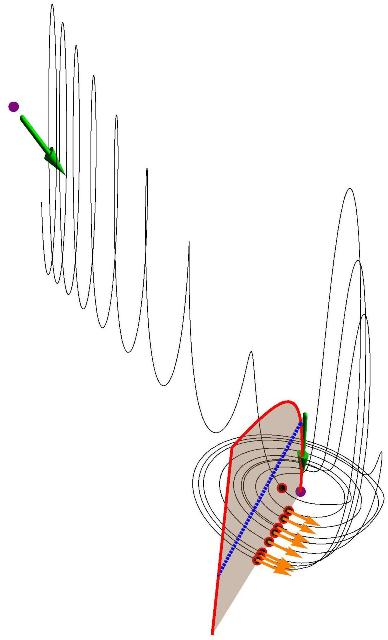
\includegraphics[width=0.25\textwidth]{RoessNeareqLbld2.jpg}
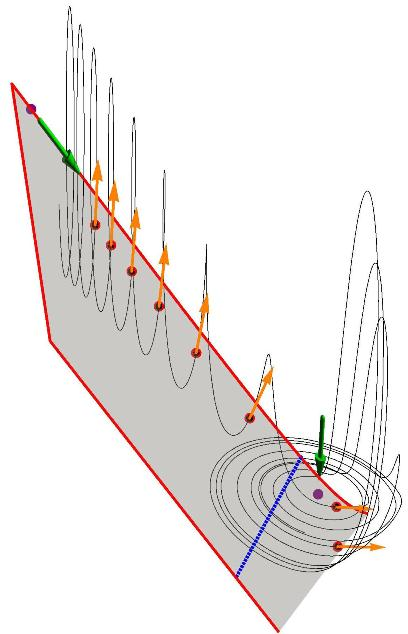
\includegraphics[width=0.25\textwidth]{RoessFareqLbld2.jpg} \\
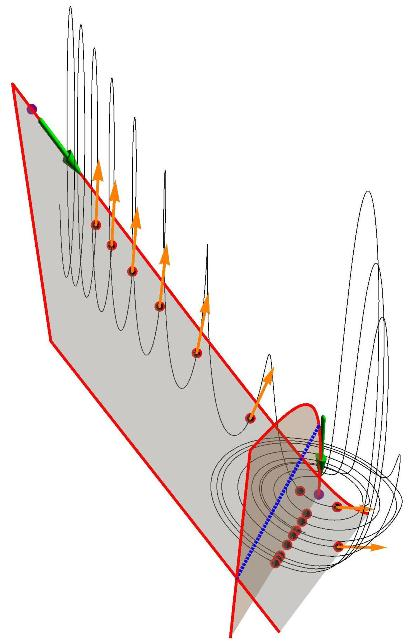
\includegraphics[width=0.25\textwidth]{RoessBotheqLbld2.jpg}
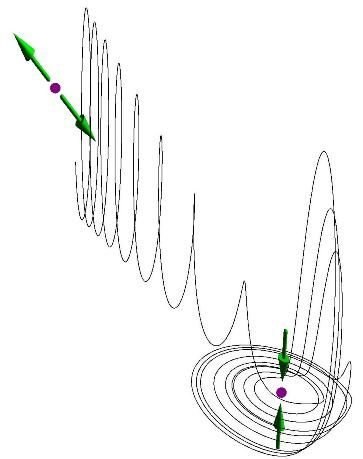
\includegraphics[width=0.25\textwidth]{RoessTrajLbld2.jpg}
\caption{R\"ossler figures fit to specifications. \label{fig:newRoss}}
\end{figure}

\item[2012-04-21 Predrag to Bryce] They are good lookers!

\item[2012-04-21 Evangelos] The Dangelmayr system\rf{Dang86} written in complex
coordinates $z_1,z_2$ reads
\begin{subequations}\label{eq:DangSO2}
\begin{align}
  \dot{z}_1 &= \mu_1\,z_1+a_1\,z_1|z_1|^2+b_1\,z_1|z_2|^2+c_1\,\overline{z}_1\,z_2\,\\
  \dot{z}_2 &= (\mu_2-\ii\, e_2)\,z_1+a_2\,z_2|z_1|^2+b_2\,z_2|z_2|^2+c_2\,z_1^2
\end{align}
\end{subequations}
(I have replaced symmetry breaking term $e$ here and in \refeq{eq:AGpolar}
with $e_2$ since in this constant is naturally paired with $\mu_2$.)
See also Armbruster, Guckenheimer and Holmes\rf{AGHO288} flow with
$\On{2}$ symmetry, Eq. \refeq{eq:AGH} above.
In \texttt{siminos/cgang/Evangelos/dangelmayr\_so2\_int.nb}
I integrate \refeq{eq:DangSO2} rather than the polar form \refeq{eq:AGpolar},
as the former has no dangerous denominators.

\item[2012-04-21 Evangelos] For future reference I note that the connection
of the constants in \refeq{eq:DangSO2} with $e_2=0$ to the constants in
equation (2.3) of \refref{Dang86} with $n=2$, $m=1$ is $\mu_1=\nu\epsilon\alpha$,
$a_1=-\nu\epsilon$, $b_1=-\nu\epsilon\rho$, $c_1=-\nu\mu$, $\mu_2=\epsilon\beta$,
$a_2=-\epsilon\kappa$, $b_2=-\epsilon\epsilon'$, $c_2=\mu\mu'$.

\item[2012-04-21 Evangelos] Our \refeq{eq:DangSO2} seems like a special case of
Porter and Knobloch\rf{PoKno05} equation (12) but some brave young gangster
has to derive the correspondence of parameters, so that we can properly cite
them. Predrag's introduction of $e_2$
seems to be the minimal modification required to break $\On{2}$ to $\SOn{2}$.
Some exploration of \refeq{eq:DangSO2}
using \texttt{siminos/cgang/Evangelos/dangelmayr\_so2\_int.nb}
shows we can have chaos, so we can stick to it. I leave it to Lei \etal\
to pick most interesting parameter values.

\item[2012-04-24 Lei] Using Evanelos' code, I found the following set of
parameters may be interesting. $\mu_1=-0.14,\mu_2=1.175,
a_1=-0.245,a_2=3.44, b_1=1.326, b_2=-0.47, c_1=1, c_2=-1, e_2=0.855$. All
the eigenvalues have positive real parts and both of the equilibrium
points have conjugate complex eigenvalues. So there is nice spirals
around them. See figure \reffig{fig:dangelmayr_proj} for projections
3-dim space.

\begin{figure}
\centering
% 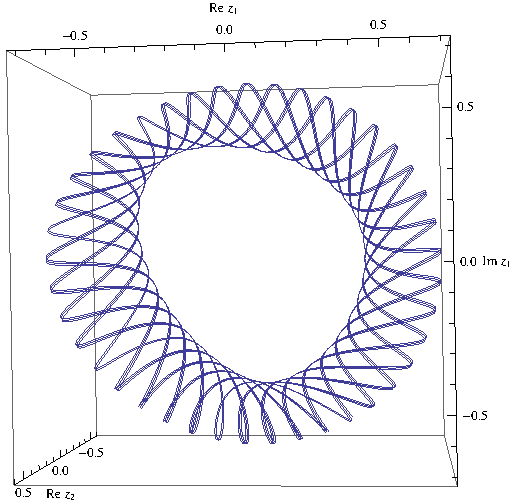
\includegraphics[width=0.35\textwidth]{dangelmayrProj}
\caption{Dangelmayr projected}
\label{fig:dangelmayr_proj}
\end{figure}

\item[2012-04-24 Predrag to Lei]

\begin{itemize}
  \item can you svn add dangelmayrProj.pdf? (using underscores in LaTeX
        files is awkward).
  \item stability eigenvalues, eigenvectors of the \eqv\ $\EQV{0}$ at
        origin, at your parameter values - if it is stable, everything
        just might fall into it and die.
  \item stability eigenvalues, eigenvectors of $\REQV{}{1}$
  \item stability eigenvalues, eigenvectors of $\REQV{}{2}$
  \item $\REQV{}{1}$: unstable eigenvalue becomes a complex
        eigenvalue pair in Cartesian coordinates?
  \item $\REQV{}{2}$: Does the unstable eigenvalue become a complex
        eigenvalue pair in Cartesian coordinates?
  \item their plots in the Cartesian coordinates
  \item $\dot{\theta}$ to see how slow/fast are they.
  \item plots of small perturbations of the above \eqv\ and \reqva\ in
        the Cartesian coordinates to see whether the dynamics looks
        chaotic
\end{itemize}

\end{description}
